\chapter{Perception results}
\label{ch.perc_res}

Originally, the intention of this study was to focus on the perception of \isi{Scouse} variants by listeners from \isi{Liverpool} and \isi{Manchester} (in order to have a rough equivalent of the oppositions Michigan-Ontario in \citealt{niedzielski1999}, and Australia-New Zealand in \citealt{hayetal2006a}).
However, I only managed to recruit 9 subjects from the \isi{Liverpool}/\isi{Merseyside} area and 3 from Greater \isi{Manchester} over the course of the 15 months that the perception test was online, despite my own best efforts and notwithstanding the fact that many people with personal contacts in \isi{Liverpool} and \isi{Manchester} helped to spread the word.
A detailed analysis of such a small sample does not seem to make much sense.
All the same, the most basic tests were carried out on the \isi{Liverpool} sub-sample as well, and, crucially, almost all results are comparable to those in the rest of the sample.
Mixed-effects ordinal models regressing reported \isi{percept} on Area (\enquote*{internal} vs. \enquote*{external}) showed that the responses given by subjects from outside were not significantly different from those provided by participants from \isi{Liverpool} as far as happ\textsc{y} (estimate = 0.025, se = 0.115, z value = 0.216, p = 0.829), \textsc{nurse} (estimate = -0.001, se = 0.185, z value = -0.007, p = 0.994), and /k/ (estimate = 0.053, se = 0.193, z value = 0.275, p = 0.783) are concerned.
This is also obvious when the relevant bar plots (not reported here) are compared with the ones generated on the basis of the `external' sample.
Furthermore, whenever there is a significant \isi{priming} effect in the \isi{Liverpool} sub-sample, this effect is in the same (unexpected) direction as the ones reported below for perceivers from outside of the city.

For velar nasal plus, on the other hand, there is a statistical trend (estimate = -0.382, se = 0.210, z value = -1.815, p = 0.070).
With respect to this variable, the difference between \isi{priming} conditions is more pronounced for subjects from \isi{Liverpool}, and the effect is in the opposite direction compared to the remaining participants from the rest of the country.
The production data suggest that velar nasal plus carries at least some social meaning, but this result \emph{could} indicate that it is actually even more \isi{salient} in \isi{Liverpool} than suspected, despite the fact that nobody comments on it.
This variable could present a fruitful area of future research, but it should be borne in mind that these statements are based on a very small and unbalanced sample, which means that we might well be talking about a non-issue because the effect would disappear in a larger dataset.

In any case, /ŋ(g)/ is the only variable where results seem to diverge.
With respect to the other three, perceivers from \isi{Liverpool} and elsewhere do not exhibit any statistically meaningful differences in behaviour.
In addition, it has been shown that impersonations and comments by outsiders have an impact on what variables Liverpudlians themselves are \isi{consciously} aware of (cf. Chapter \ref{prod.res.qual}), so internal and external \isi{salience} correlate to a degree and are not completely unrelated.
For these reason I would argue that it does not appear completely unjustified to assume that most of what is described below would also hold in a larger sample of listeners from \isi{Liverpool}, but this claim is in need of proper empirical confirmation in the future.
All further results reported in this chapter are exclusively based on responses provided by people living outside of \isi{Liverpool}.

\section{happ\textrm{\textsc{y}}}
\label{sec.perc_res.happy}
	\subsection{Overview}
	\label{sec.perc_res.happy.overview}

As described in Section \ref{sec.perc_method.stats}, a mixed-effects ordinal regression model was fit to the data by hand.
This maximal model did not contain any troubling \isi{collinearity} (κ = 13.99), but for reasons of comparability (cf. \ref{sec.perc_res.nurse}, \ref{sec.perc_res.ng}, and \ref{sec.perc_res.k}), the frequency of the keyword expressed in \isi{Zipf} scores, as well as the interaction of \isi{Zipf} score and \isi{priming} condition, were removed from the model.\footnote{When \isi{Zipf} scores are included they show up as a significant predictor in the corresponding minimal adequate model (p < 0.001). The same is true for position of keyword (p < 0.001) and age of participant (p = 0.043). In addition, \isi{geographical distance} from \isi{Liverpool} almost reaches statistical significance as well (p = 0.080). Frequency and age are therefore briefly discussed below for the sake of completeness.}
\isi{Collinearity} was further reduced this way (κ = 10.61).
Model selection based on AIC scores and F-tests comparing nested models resulted in the minimal adequate model printed below.
Only two factors show up as main effects (one of them not quite significant) and no statistically significant interactions could be found.
Position of the stimulus (in the middle or at the end of the sentence) is a highly significant predictor.
Geographical distance of the participant from \isi{Liverpool} does not reach significance at the 5\% level, but the p-value is low enough to qualify as a statistical trend.
For this reason the factor was kept in the model.

\begin{table}[h]
	\caption{happ\textsc{y} (perception): mixed-effects ordinal regression}
	\centering
	\begin{tabular}{p{0.2\textwidth}rrrrl}
		\hline
		Fixed effects: & Estimate & Std. Error &  z value & Pr($>$$|$z$|$) & \\ 
		\hline
		Position[final] & -0.932 & 0.091 & -10.194 & <0.001 & ***\\ 
		Distance & 0.169 & 0.093 & 1.811 & 0.070 & .\\ 
		\hline
		Random effects: & & & &\\
		Groups &         Name & Variance &      Std.Dev. & & \\
		Questionnaire &  (Intercept) & 0.162 & 0.402 & & \\
		Questionnaire & Token      & <0.001 & <0.001 & & \\
		\multicolumn{3}{l}{(number of obs: 516, groups: Questionnaire, 55)} & & \\
		\hline
	\end{tabular}
\end{table}

\subsection{Prime}
\label{sec.perc_res.happy.prime}

Prime is not among the fixed effects.
This indicates that for the happ\textsc{y} stimuli it did not make a difference whether participants thought they were listening to a speaker from \isi{Liverpool} or \isi{Manchester}.
Figure \ref{fig.bar.happy.tot.ext} visualises this fact.
As with all the following bar plots in this chapter, answers from subjects who were primed for ``\isi{Liverpool}'' are represented by black bars, those given by people who were correctly told the speaker was from \isi{Manchester} are visualised by light grey bars.

\begin{figure}[h]
	\centering
		\definecolor{shadecolor}{rgb}{0.969, 0.969, 0.969}
		\resizebox{.49\linewidth}{!}{% Created by tikzDevice version 0.10.1 on 2017-04-14 13:58:29
% !TEX encoding = UTF-8 Unicode
\begin{tikzpicture}[x=1pt,y=1pt]
\definecolor{fillColor}{RGB}{255,255,255}
\path[use as bounding box,fill=fillColor,fill opacity=0.00] (0,0) rectangle (505.89,505.89);
\begin{scope}
\path[clip] (  0.00,  0.00) rectangle (505.89,505.89);
\definecolor{drawColor}{RGB}{255,255,255}
\definecolor{fillColor}{RGB}{255,255,255}

\path[draw=drawColor,line width= 0.6pt,line join=round,line cap=round,fill=fillColor] (  0.00,  0.00) rectangle (505.89,505.89);
\end{scope}
\begin{scope}
\path[clip] ( 64.22, 62.51) rectangle (500.39,462.54);
\definecolor{fillColor}{RGB}{255,255,255}

\path[fill=fillColor] ( 64.22, 62.51) rectangle (500.39,462.54);
\definecolor{drawColor}{gray}{0.92}

\path[draw=drawColor,line width= 0.3pt,line join=round] ( 64.22,126.16) --
	(500.39,126.16);

\path[draw=drawColor,line width= 0.3pt,line join=round] ( 64.22,217.07) --
	(500.39,217.07);

\path[draw=drawColor,line width= 0.3pt,line join=round] ( 64.22,307.99) --
	(500.39,307.99);

\path[draw=drawColor,line width= 0.3pt,line join=round] ( 64.22,398.90) --
	(500.39,398.90);

\path[draw=drawColor,line width= 0.6pt,line join=round] ( 64.22, 80.70) --
	(500.39, 80.70);

\path[draw=drawColor,line width= 0.6pt,line join=round] ( 64.22,171.61) --
	(500.39,171.61);

\path[draw=drawColor,line width= 0.6pt,line join=round] ( 64.22,262.53) --
	(500.39,262.53);

\path[draw=drawColor,line width= 0.6pt,line join=round] ( 64.22,353.44) --
	(500.39,353.44);

\path[draw=drawColor,line width= 0.6pt,line join=round] ( 64.22,444.36) --
	(500.39,444.36);

\path[draw=drawColor,line width= 0.6pt,line join=round] (126.53, 62.51) --
	(126.53,462.54);

\path[draw=drawColor,line width= 0.6pt,line join=round] (230.38, 62.51) --
	(230.38,462.54);

\path[draw=drawColor,line width= 0.6pt,line join=round] (334.23, 62.51) --
	(334.23,462.54);

\path[draw=drawColor,line width= 0.6pt,line join=round] (438.08, 62.51) --
	(438.08,462.54);
\definecolor{fillColor}{gray}{0.80}

\path[fill=fillColor] (126.53, 80.70) rectangle (173.26,179.13);
\definecolor{fillColor}{gray}{0.20}

\path[fill=fillColor] ( 79.80, 80.70) rectangle (126.53,183.18);
\definecolor{fillColor}{gray}{0.80}

\path[fill=fillColor] (230.38, 80.70) rectangle (277.11,231.03);
\definecolor{fillColor}{gray}{0.20}

\path[fill=fillColor] (183.65, 80.70) rectangle (230.38,242.69);
\definecolor{fillColor}{gray}{0.80}

\path[fill=fillColor] (334.23, 80.70) rectangle (380.96,214.92);
\definecolor{fillColor}{gray}{0.20}

\path[fill=fillColor] (287.50, 80.70) rectangle (334.23,209.63);
\definecolor{fillColor}{gray}{0.80}

\path[fill=fillColor] (438.08, 80.70) rectangle (484.81,152.28);
\definecolor{fillColor}{gray}{0.20}

\path[fill=fillColor] (391.35, 80.70) rectangle (438.08,141.86);
\definecolor{drawColor}{gray}{0.20}

\path[draw=drawColor,line width= 0.6pt,line join=round,line cap=round] ( 64.22, 62.51) rectangle (500.39,462.54);
\end{scope}
\begin{scope}
\path[clip] (  0.00,  0.00) rectangle (505.89,505.89);
\definecolor{drawColor}{gray}{0.30}

\node[text=drawColor,anchor=base east,inner sep=0pt, outer sep=0pt, scale=  1.60] at ( 59.27, 74.66) {0{\%}};

\node[text=drawColor,anchor=base east,inner sep=0pt, outer sep=0pt, scale=  1.60] at ( 59.27,165.58) {20{\%}};

\node[text=drawColor,anchor=base east,inner sep=0pt, outer sep=0pt, scale=  1.60] at ( 59.27,256.49) {40{\%}};

\node[text=drawColor,anchor=base east,inner sep=0pt, outer sep=0pt, scale=  1.60] at ( 59.27,347.41) {60{\%}};

\node[text=drawColor,anchor=base east,inner sep=0pt, outer sep=0pt, scale=  1.60] at ( 59.27,438.32) {80{\%}};
\end{scope}
\begin{scope}
\path[clip] (  0.00,  0.00) rectangle (505.89,505.89);
\definecolor{drawColor}{gray}{0.20}

\path[draw=drawColor,line width= 0.6pt,line join=round] ( 61.47, 80.70) --
	( 64.22, 80.70);

\path[draw=drawColor,line width= 0.6pt,line join=round] ( 61.47,171.61) --
	( 64.22,171.61);

\path[draw=drawColor,line width= 0.6pt,line join=round] ( 61.47,262.53) --
	( 64.22,262.53);

\path[draw=drawColor,line width= 0.6pt,line join=round] ( 61.47,353.44) --
	( 64.22,353.44);

\path[draw=drawColor,line width= 0.6pt,line join=round] ( 61.47,444.36) --
	( 64.22,444.36);
\end{scope}
\begin{scope}
\path[clip] (  0.00,  0.00) rectangle (505.89,505.89);
\definecolor{drawColor}{gray}{0.20}

\path[draw=drawColor,line width= 0.6pt,line join=round] (126.53, 59.76) --
	(126.53, 62.51);

\path[draw=drawColor,line width= 0.6pt,line join=round] (230.38, 59.76) --
	(230.38, 62.51);

\path[draw=drawColor,line width= 0.6pt,line join=round] (334.23, 59.76) --
	(334.23, 62.51);

\path[draw=drawColor,line width= 0.6pt,line join=round] (438.08, 59.76) --
	(438.08, 62.51);
\end{scope}
\begin{scope}
\path[clip] (  0.00,  0.00) rectangle (505.89,505.89);
\definecolor{drawColor}{gray}{0.30}

\node[text=drawColor,anchor=base,inner sep=0pt, outer sep=0pt, scale=  1.60] at (126.53, 45.50) {1 [ə]};

\node[text=drawColor,anchor=base,inner sep=0pt, outer sep=0pt, scale=  1.60] at (126.53, 28.22) { ←more Manchester};

\node[text=drawColor,anchor=base,inner sep=0pt, outer sep=0pt, scale=  1.60] at (230.38, 45.50) {2 [ɪ]};

\node[text=drawColor,anchor=base,inner sep=0pt, outer sep=0pt, scale=  1.60] at (334.23, 45.50) {3 [ï]};

\node[text=drawColor,anchor=base,inner sep=0pt, outer sep=0pt, scale=  1.60] at (438.08, 45.50) {4 [i]};

\node[text=drawColor,anchor=base,inner sep=0pt, outer sep=0pt, scale=  1.60] at (438.08, 28.22) { more Liverpool→};
\end{scope}
\begin{scope}
\path[clip] (  0.00,  0.00) rectangle (505.89,505.89);
\definecolor{drawColor}{RGB}{0,0,0}

\node[text=drawColor,anchor=base,inner sep=0pt, outer sep=0pt, scale=  2.00] at (282.31,  7.63) {reported percept};
\end{scope}
\begin{scope}
\path[clip] (  0.00,  0.00) rectangle (505.89,505.89);
\definecolor{drawColor}{RGB}{0,0,0}

\node[text=drawColor,rotate= 90.00,anchor=base,inner sep=0pt, outer sep=0pt, scale=  2.00] at ( 20.59,262.53) {of cases};
\end{scope}
\begin{scope}
\path[clip] (  0.00,  0.00) rectangle (505.89,505.89);
\definecolor{fillColor}{RGB}{255,255,255}

\path[fill=fillColor] (130.20,473.92) rectangle (434.41,500.39);
\end{scope}
\begin{scope}
\path[clip] (  0.00,  0.00) rectangle (505.89,505.89);
\definecolor{drawColor}{RGB}{0,0,0}

\node[text=drawColor,anchor=base west,inner sep=0pt, outer sep=0pt, scale=  2.00] at (135.89,479.61) {prime};
\end{scope}
\begin{scope}
\path[clip] (  0.00,  0.00) rectangle (505.89,505.89);
\definecolor{fillColor}{RGB}{255,255,255}

\path[fill=fillColor] (194.31,479.61) rectangle (208.77,494.70);
\end{scope}
\begin{scope}
\path[clip] (  0.00,  0.00) rectangle (505.89,505.89);
\definecolor{fillColor}{gray}{0.20}

\path[fill=fillColor] (195.02,480.32) rectangle (208.05,493.99);
\end{scope}
\begin{scope}
\path[clip] (  0.00,  0.00) rectangle (505.89,505.89);
\definecolor{fillColor}{RGB}{255,255,255}

\path[fill=fillColor] (302.78,479.61) rectangle (317.23,494.70);
\end{scope}
\begin{scope}
\path[clip] (  0.00,  0.00) rectangle (505.89,505.89);
\definecolor{fillColor}{gray}{0.80}

\path[fill=fillColor] (303.49,480.32) rectangle (316.52,493.99);
\end{scope}
\begin{scope}
\path[clip] (  0.00,  0.00) rectangle (505.89,505.89);
\definecolor{drawColor}{RGB}{0,0,0}

\node[text=drawColor,anchor=base west,inner sep=0pt, outer sep=0pt, scale=  2.00] at (210.57,479.61) {Liverpool};
\end{scope}
\begin{scope}
\path[clip] (  0.00,  0.00) rectangle (505.89,505.89);
\definecolor{drawColor}{RGB}{0,0,0}

\node[text=drawColor,anchor=base west,inner sep=0pt, outer sep=0pt, scale=  2.00] at (319.04,479.61) {Manchester};
\end{scope}
\end{tikzpicture}
} 
	\caption{happ\textsc{y} (perception) by prime}
	\label{fig.bar.happy.tot.ext}
\end{figure}

There is a slight preference for stimulus number 2 (the one actually present in the stimulus sentences) at around 35\% of answers given, followed by the somewhat tenser (and more Liverpool-like) stimulus 3 at just below 30\%.
The `hyper-\isi{Mancunian}' and `hyper-\isi{Liverpool}' stimuli 1 (about 20\%) and 4 (15--17\%) were less frequently chosen.
The crucial point, however, is that only marginal differences between the two conditions are visible, which corroborates the result of the mixed-effects model that subjects were not influenced by the \isi{prime} when perceiving happ\textsc{y}-stimuli.

\subsection{Position of carrier word}
\label{sec.perc_res.happy.position}

Figure \ref{fig.bar.happy.tot.ext.pos} shows the clear influence of carrier word position within the stimulus sentence that was identified as a significant predictor by the mixed-effects model.
Perception of sentence-final stimuli can be said to be more objective as participants chose stimulus 2 (which actually occurred in the recording) in around 45\% of cases.
The hyper-centralised stimulus 1 was, at about 35\%, also quite frequent, whereas the `\isi{Liverpool}' stimuli 3 and 4 only account for 20\% of answers, with stimulus 4 being particularly rare.
When the carrier word was presented in the middle of the sentence, subjects most often reported having heard stimulus number 3, a \isi{vowel} higher and fronter than in the actual recording.
Stimuli 2 and 4 were both chosen around 25--30\% of the time, while the hyper-\isi{Mancunian} \isi{vowel} was only selected in a bit more than 10\% of cases.
Overall then, participants were more likely to perceive a `\isi{Liverpool}'-type tenser /i/ when the carrier word was presented in the middle of the sentence than when it occurred as the last word in the sentence.

\begin{figure}[h]
	\centering
	\begin{subfigure}{0.49\textwidth}
		\centering
			\definecolor{shadecolor}{rgb}{0.969, 0.969, 0.969}
			\resizebox{\linewidth}{!}{\input{figures/bar_happy_ext_med-1.tikz}} 
		\caption{medial}
		\label{fig.bar.happy.tot.ext.med}
	\end{subfigure}
	\begin{subfigure}{0.49\textwidth}
		\centering
			\definecolor{shadecolor}{rgb}{0.969, 0.969, 0.969}
			\resizebox{\linewidth}{!}{\input{figures/bar_happy_ext_fin-1.tikz}} 
		\caption{final}
		\label{fig.bar.happy.tot.ext.fin}
	\end{subfigure}
	\caption{happ\textsc{y} (perception) by position}
	\label{fig.bar.happy.tot.ext.pos}
\end{figure}

It is dubious, however, whether this difference is due to the fact that subjects have to hold the relevant sound in memory --- which would be what the different stimulus sentences were meant to test (cf. Section \ref{sec.perc_method.sentences}).
It seems at least as plausible that the effect is caused by the acoustic material.
In \isi{Mancunian} English, happ\textsc{y} is typically realised as [ɪ] in phrase-medial and [ə] in phrase-final position, and the stimulus sentences used in this experiment were authentic in this respect (cf. \ref{sec.perc_method.sentences}).
The happ\textsc{y} realisations were thus more central when the word occurred at the end of the sentence than when it appeared in the middle of it.
It is possible that participants picked up on this difference in realisation and hyper-corrected by selecting one of the tenser answer options when the carrier word was sentence-medially, simply because the \isi{vowel} sounded tenser than the one they encountered in the sentence-final stimuli.

Another option is that the difference due to word position is an artefact of the method of stimulus creation.
Since satisfactory continua could not be \isi{resynthesised} out of many phrase-final happ\textsc{y} vowels, the continua \isi{resynthesised} on the basis of the same words presented in a sentence-medial context were used as answer options instead (cf. \ref{sec.perc_method.vow}).
This meant that, for sentence-final happ\textsc{y} stimuli, answer option 2 was a bit tenser than the \isi{vowel} actually present in the sentence.
In this interpretation then, subjects would have reacted quite similarly for both sentence-medial and sentence-final stimuli --- most often choosing an answer option that was a bit tenser than the \isi{vowel} they had actually heard.
The only difference would then be that for phrase-final sentences stimulus 2 already fulfilled this criterion, whereas for phrase-medial sentences it was not before stimulus 3 that participants encountered a \isi{vowel} that was tenser than the one contained in the carrier word.

In any case, position of the stimulus does not show up in the mixed-effects model because of \isi{priming} which only occurred in one context but not in the other (if this was the case the model should have revealed a significant interaction of \isi{prime} and position).
This is also visible in Figures \ref{fig.bar.happy.tot.ext.fin} and \ref{fig.bar.happy.tot.ext.med}, none of which show pronounced differences between \isi{priming} conditions.

\subsection{Geographical distance}
\label{sec.perc_res.happy.geography}

\begin{figure}[h]
	\centering
		\definecolor{shadecolor}{rgb}{0.969, 0.969, 0.969}
		\resizebox{.49\linewidth}{!}{% Created by tikzDevice version 0.8.1 on 2016-02-09 02:18:13
% !TEX encoding = UTF-8 Unicode
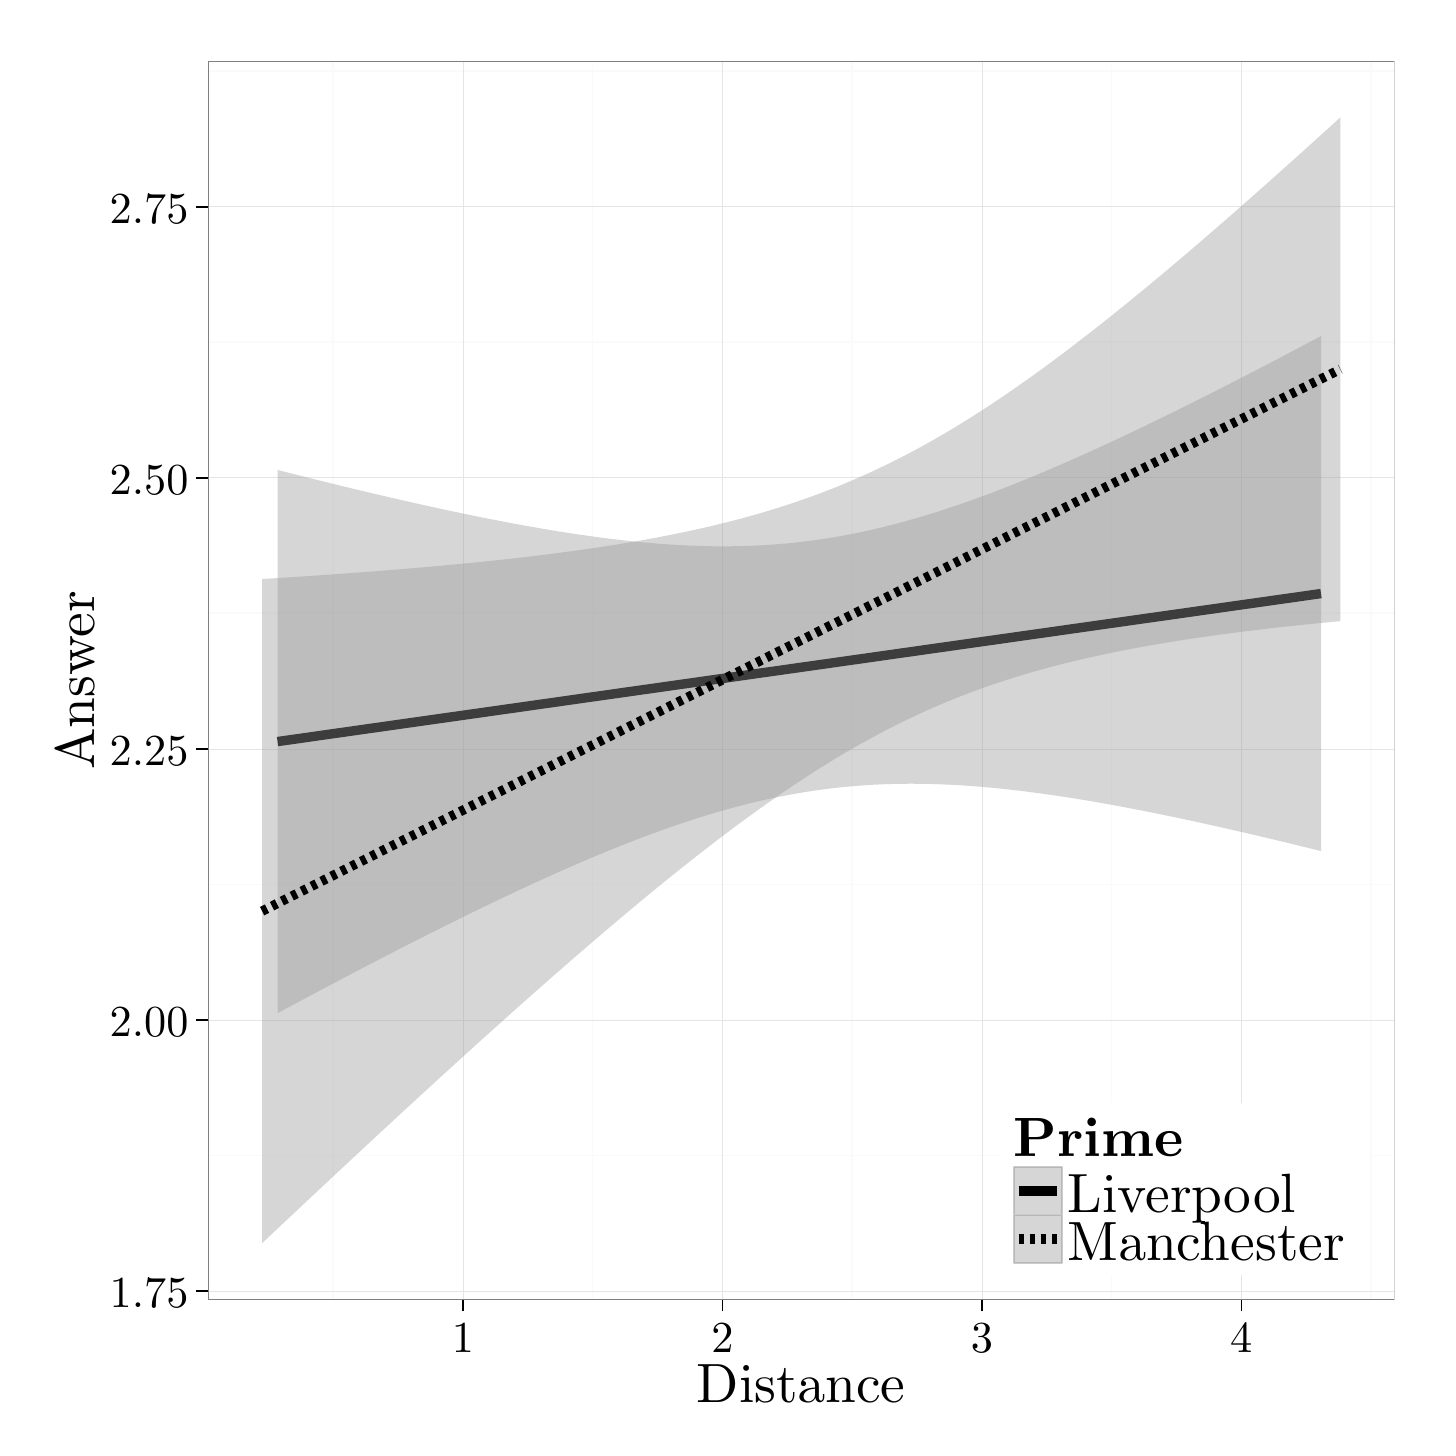
\begin{tikzpicture}[x=1pt,y=1pt]
\definecolor{fillColor}{RGB}{255,255,255}
\path[use as bounding box,fill=fillColor,fill opacity=0.00] (0,0) rectangle (505.89,505.89);
\begin{scope}
\path[clip] (  0.00,  0.00) rectangle (505.89,505.89);
\definecolor{drawColor}{RGB}{255,255,255}
\definecolor{fillColor}{RGB}{255,255,255}

\path[draw=drawColor,line width= 0.6pt,line join=round,line cap=round,fill=fillColor] (  0.00, -0.00) rectangle (505.89,505.89);
\end{scope}
\begin{scope}
\path[clip] ( 65.21, 46.31) rectangle (493.85,493.84);
\definecolor{fillColor}{RGB}{255,255,255}

\path[fill=fillColor] ( 65.21, 46.31) rectangle (493.85,493.84);
\definecolor{drawColor}{gray}{0.98}

\path[draw=drawColor,line width= 0.6pt,line join=round] ( 65.21, 98.38) --
	(493.85, 98.38);

\path[draw=drawColor,line width= 0.6pt,line join=round] ( 65.21,196.33) --
	(493.85,196.33);

\path[draw=drawColor,line width= 0.6pt,line join=round] ( 65.21,294.28) --
	(493.85,294.28);

\path[draw=drawColor,line width= 0.6pt,line join=round] ( 65.21,392.22) --
	(493.85,392.22);

\path[draw=drawColor,line width= 0.6pt,line join=round] ( 65.21,490.17) --
	(493.85,490.17);

\path[draw=drawColor,line width= 0.6pt,line join=round] (110.39, 46.31) --
	(110.39,493.84);

\path[draw=drawColor,line width= 0.6pt,line join=round] (204.15, 46.31) --
	(204.15,493.84);

\path[draw=drawColor,line width= 0.6pt,line join=round] (297.91, 46.31) --
	(297.91,493.84);

\path[draw=drawColor,line width= 0.6pt,line join=round] (391.67, 46.31) --
	(391.67,493.84);

\path[draw=drawColor,line width= 0.6pt,line join=round] (485.43, 46.31) --
	(485.43,493.84);
\definecolor{drawColor}{gray}{0.90}

\path[draw=drawColor,line width= 0.2pt,line join=round] ( 65.21, 49.41) --
	(493.85, 49.41);

\path[draw=drawColor,line width= 0.2pt,line join=round] ( 65.21,147.36) --
	(493.85,147.36);

\path[draw=drawColor,line width= 0.2pt,line join=round] ( 65.21,245.30) --
	(493.85,245.30);

\path[draw=drawColor,line width= 0.2pt,line join=round] ( 65.21,343.25) --
	(493.85,343.25);

\path[draw=drawColor,line width= 0.2pt,line join=round] ( 65.21,441.20) --
	(493.85,441.20);

\path[draw=drawColor,line width= 0.2pt,line join=round] (157.27, 46.31) --
	(157.27,493.84);

\path[draw=drawColor,line width= 0.2pt,line join=round] (251.03, 46.31) --
	(251.03,493.84);

\path[draw=drawColor,line width= 0.2pt,line join=round] (344.79, 46.31) --
	(344.79,493.84);

\path[draw=drawColor,line width= 0.2pt,line join=round] (438.55, 46.31) --
	(438.55,493.84);
\definecolor{fillColor}{RGB}{153,153,153}

\path[fill=fillColor,fill opacity=0.40] ( 90.29,346.06) --
	( 95.06,344.85) --
	( 99.83,343.65) --
	(104.61,342.46) --
	(109.38,341.29) --
	(114.15,340.12) --
	(118.92,338.97) --
	(123.70,337.83) --
	(128.47,336.71) --
	(133.24,335.61) --
	(138.02,334.52) --
	(142.79,333.45) --
	(147.56,332.40) --
	(152.33,331.37) --
	(157.11,330.36) --
	(161.88,329.38) --
	(166.65,328.42) --
	(171.43,327.49) --
	(176.20,326.59) --
	(180.97,325.72) --
	(185.74,324.88) --
	(190.52,324.08) --
	(195.29,323.32) --
	(200.06,322.61) --
	(204.84,321.93) --
	(209.61,321.31) --
	(214.38,320.74) --
	(219.15,320.22) --
	(223.93,319.76) --
	(228.70,319.37) --
	(233.47,319.04) --
	(238.24,318.78) --
	(243.02,318.60) --
	(247.79,318.49) --
	(252.56,318.47) --
	(257.34,318.54) --
	(262.11,318.69) --
	(266.88,318.94) --
	(271.65,319.28) --
	(276.43,319.72) --
	(281.20,320.26) --
	(285.97,320.91) --
	(290.75,321.65) --
	(295.52,322.49) --
	(300.29,323.43) --
	(305.06,324.47) --
	(309.84,325.60) --
	(314.61,326.82) --
	(319.38,328.14) --
	(324.16,329.54) --
	(328.93,331.02) --
	(333.70,332.58) --
	(338.47,334.21) --
	(343.25,335.91) --
	(348.02,337.68) --
	(352.79,339.51) --
	(357.56,341.40) --
	(362.34,343.34) --
	(367.11,345.33) --
	(371.88,347.37) --
	(376.66,349.45) --
	(381.43,351.58) --
	(386.20,353.74) --
	(390.97,355.94) --
	(395.75,358.17) --
	(400.52,360.44) --
	(405.29,362.73) --
	(410.07,365.05) --
	(414.84,367.39) --
	(419.61,369.76) --
	(424.38,372.15) --
	(429.16,374.56) --
	(433.93,376.99) --
	(438.70,379.44) --
	(443.47,381.90) --
	(448.25,384.38) --
	(453.02,386.88) --
	(457.79,389.39) --
	(462.57,391.91) --
	(467.34,394.44) --
	(467.34,208.35) --
	(462.57,209.53) --
	(457.79,210.70) --
	(453.02,211.86) --
	(448.25,213.00) --
	(443.47,214.12) --
	(438.70,215.23) --
	(433.93,216.33) --
	(429.16,217.40) --
	(424.38,218.46) --
	(419.61,219.50) --
	(414.84,220.51) --
	(410.07,221.50) --
	(405.29,222.47) --
	(400.52,223.40) --
	(395.75,224.31) --
	(390.97,225.19) --
	(386.20,226.04) --
	(381.43,226.85) --
	(376.66,227.62) --
	(371.88,228.35) --
	(367.11,229.03) --
	(362.34,229.67) --
	(357.56,230.26) --
	(352.79,230.79) --
	(348.02,231.27) --
	(343.25,231.68) --
	(338.47,232.03) --
	(333.70,232.31) --
	(328.93,232.51) --
	(324.16,232.64) --
	(319.38,232.69) --
	(314.61,232.65) --
	(309.84,232.52) --
	(305.06,232.30) --
	(300.29,231.98) --
	(295.52,231.57) --
	(290.75,231.05) --
	(285.97,230.44) --
	(281.20,229.73) --
	(276.43,228.92) --
	(271.65,228.00) --
	(266.88,226.99) --
	(262.11,225.89) --
	(257.34,224.69) --
	(252.56,223.40) --
	(247.79,222.02) --
	(243.02,220.57) --
	(238.24,219.03) --
	(233.47,217.42) --
	(228.70,215.73) --
	(223.93,213.99) --
	(219.15,212.17) --
	(214.38,210.30) --
	(209.61,208.37) --
	(204.84,206.40) --
	(200.06,204.37) --
	(195.29,202.30) --
	(190.52,200.18) --
	(185.74,198.03) --
	(180.97,195.84) --
	(176.20,193.62) --
	(171.43,191.36) --
	(166.65,189.08) --
	(161.88,186.77) --
	(157.11,184.43) --
	(152.33,182.07) --
	(147.56,179.69) --
	(142.79,177.28) --
	(138.02,174.86) --
	(133.24,172.42) --
	(128.47,169.96) --
	(123.70,167.48) --
	(118.92,164.99) --
	(114.15,162.48) --
	(109.38,159.97) --
	(104.61,157.44) --
	( 99.83,154.89) --
	( 95.06,152.34) --
	( 90.29,149.78) --
	cycle;
\definecolor{drawColor}{RGB}{0,0,0}

\path[draw=drawColor,line width= 3.4pt,line join=round] ( 90.29,247.92) --
	( 95.06,248.59) --
	( 99.83,249.27) --
	(104.61,249.95) --
	(109.38,250.63) --
	(114.15,251.30) --
	(118.92,251.98) --
	(123.70,252.66) --
	(128.47,253.33) --
	(133.24,254.01) --
	(138.02,254.69) --
	(142.79,255.36) --
	(147.56,256.04) --
	(152.33,256.72) --
	(157.11,257.40) --
	(161.88,258.07) --
	(166.65,258.75) --
	(171.43,259.43) --
	(176.20,260.10) --
	(180.97,260.78) --
	(185.74,261.46) --
	(190.52,262.13) --
	(195.29,262.81) --
	(200.06,263.49) --
	(204.84,264.17) --
	(209.61,264.84) --
	(214.38,265.52) --
	(219.15,266.20) --
	(223.93,266.87) --
	(228.70,267.55) --
	(233.47,268.23) --
	(238.24,268.90) --
	(243.02,269.58) --
	(247.79,270.26) --
	(252.56,270.93) --
	(257.34,271.61) --
	(262.11,272.29) --
	(266.88,272.97) --
	(271.65,273.64) --
	(276.43,274.32) --
	(281.20,275.00) --
	(285.97,275.67) --
	(290.75,276.35) --
	(295.52,277.03) --
	(300.29,277.70) --
	(305.06,278.38) --
	(309.84,279.06) --
	(314.61,279.74) --
	(319.38,280.41) --
	(324.16,281.09) --
	(328.93,281.77) --
	(333.70,282.44) --
	(338.47,283.12) --
	(343.25,283.80) --
	(348.02,284.47) --
	(352.79,285.15) --
	(357.56,285.83) --
	(362.34,286.51) --
	(367.11,287.18) --
	(371.88,287.86) --
	(376.66,288.54) --
	(381.43,289.21) --
	(386.20,289.89) --
	(390.97,290.57) --
	(395.75,291.24) --
	(400.52,291.92) --
	(405.29,292.60) --
	(410.07,293.27) --
	(414.84,293.95) --
	(419.61,294.63) --
	(424.38,295.31) --
	(429.16,295.98) --
	(433.93,296.66) --
	(438.70,297.34) --
	(443.47,298.01) --
	(448.25,298.69) --
	(453.02,299.37) --
	(457.79,300.04) --
	(462.57,300.72) --
	(467.34,301.40);

\path[fill=fillColor,fill opacity=0.40] ( 84.70,306.65) --
	( 89.63,306.96) --
	( 94.56,307.27) --
	( 99.49,307.59) --
	(104.43,307.93) --
	(109.36,308.27) --
	(114.29,308.62) --
	(119.22,308.98) --
	(124.16,309.35) --
	(129.09,309.74) --
	(134.02,310.14) --
	(138.95,310.55) --
	(143.89,310.97) --
	(148.82,311.41) --
	(153.75,311.87) --
	(158.68,312.34) --
	(163.62,312.84) --
	(168.55,313.35) --
	(173.48,313.88) --
	(178.41,314.44) --
	(183.35,315.02) --
	(188.28,315.63) --
	(193.21,316.27) --
	(198.14,316.93) --
	(203.08,317.63) --
	(208.01,318.37) --
	(212.94,319.14) --
	(217.87,319.95) --
	(222.81,320.81) --
	(227.74,321.72) --
	(232.67,322.68) --
	(237.60,323.69) --
	(242.54,324.76) --
	(247.47,325.89) --
	(252.40,327.10) --
	(257.33,328.37) --
	(262.27,329.73) --
	(267.20,331.16) --
	(272.13,332.69) --
	(277.06,334.30) --
	(282.00,336.02) --
	(286.93,337.83) --
	(291.86,339.75) --
	(296.79,341.79) --
	(301.73,343.93) --
	(306.66,346.19) --
	(311.59,348.57) --
	(316.52,351.06) --
	(321.46,353.67) --
	(326.39,356.40) --
	(331.32,359.24) --
	(336.25,362.19) --
	(341.19,365.26) --
	(346.12,368.43) --
	(351.05,371.69) --
	(355.98,375.06) --
	(360.92,378.52) --
	(365.85,382.06) --
	(370.78,385.68) --
	(375.71,389.38) --
	(380.64,393.16) --
	(385.58,396.99) --
	(390.51,400.90) --
	(395.44,404.86) --
	(400.37,408.87) --
	(405.31,412.93) --
	(410.24,417.05) --
	(415.17,421.20) --
	(420.10,425.39) --
	(425.04,429.63) --
	(429.97,433.89) --
	(434.90,438.19) --
	(439.83,442.52) --
	(444.77,446.88) --
	(449.70,451.26) --
	(454.63,455.67) --
	(459.56,460.09) --
	(464.50,464.54) --
	(469.43,469.01) --
	(474.36,473.50) --
	(474.36,291.45) --
	(469.43,290.98) --
	(464.50,290.50) --
	(459.56,289.99) --
	(454.63,289.46) --
	(449.70,288.91) --
	(444.77,288.33) --
	(439.83,287.73) --
	(434.90,287.10) --
	(429.97,286.44) --
	(425.04,285.75) --
	(420.10,285.03) --
	(415.17,284.26) --
	(410.24,283.46) --
	(405.31,282.61) --
	(400.37,281.72) --
	(395.44,280.78) --
	(390.51,279.78) --
	(385.58,278.72) --
	(380.64,277.60) --
	(375.71,276.42) --
	(370.78,275.16) --
	(365.85,273.83) --
	(360.92,272.41) --
	(355.98,270.91) --
	(351.05,269.32) --
	(346.12,267.63) --
	(341.19,265.84) --
	(336.25,263.95) --
	(331.32,261.94) --
	(326.39,259.83) --
	(321.46,257.60) --
	(316.52,255.25) --
	(311.59,252.79) --
	(306.66,250.20) --
	(301.73,247.51) --
	(296.79,244.69) --
	(291.86,241.77) --
	(286.93,238.73) --
	(282.00,235.59) --
	(277.06,232.35) --
	(272.13,229.00) --
	(267.20,225.57) --
	(262.27,222.05) --
	(257.33,218.45) --
	(252.40,214.76) --
	(247.47,211.01) --
	(242.54,207.19) --
	(237.60,203.30) --
	(232.67,199.35) --
	(227.74,195.35) --
	(222.81,191.30) --
	(217.87,187.20) --
	(212.94,183.06) --
	(208.01,178.87) --
	(203.08,174.65) --
	(198.14,170.39) --
	(193.21,166.10) --
	(188.28,161.78) --
	(183.35,157.43) --
	(178.41,153.05) --
	(173.48,148.65) --
	(168.55,144.23) --
	(163.62,139.79) --
	(158.68,135.32) --
	(153.75,130.84) --
	(148.82,126.34) --
	(143.89,121.82) --
	(138.95,117.29) --
	(134.02,112.74) --
	(129.09,108.18) --
	(124.16,103.61) --
	(119.22, 99.02) --
	(114.29, 94.43) --
	(109.36, 89.82) --
	(104.43, 85.20) --
	( 99.49, 80.58) --
	( 94.56, 75.94) --
	( 89.63, 71.30) --
	( 84.70, 66.65) --
	cycle;

\path[draw=drawColor,line width= 3.4pt,dash pattern=on 2pt off 2pt ,line join=round] ( 84.70,186.65) --
	( 89.63,189.13) --
	( 94.56,191.61) --
	( 99.49,194.09) --
	(104.43,196.57) --
	(109.36,199.04) --
	(114.29,201.52) --
	(119.22,204.00) --
	(124.16,206.48) --
	(129.09,208.96) --
	(134.02,211.44) --
	(138.95,213.92) --
	(143.89,216.40) --
	(148.82,218.87) --
	(153.75,221.35) --
	(158.68,223.83) --
	(163.62,226.31) --
	(168.55,228.79) --
	(173.48,231.27) --
	(178.41,233.75) --
	(183.35,236.23) --
	(188.28,238.71) --
	(193.21,241.18) --
	(198.14,243.66) --
	(203.08,246.14) --
	(208.01,248.62) --
	(212.94,251.10) --
	(217.87,253.58) --
	(222.81,256.06) --
	(227.74,258.54) --
	(232.67,261.01) --
	(237.60,263.49) --
	(242.54,265.97) --
	(247.47,268.45) --
	(252.40,270.93) --
	(257.33,273.41) --
	(262.27,275.89) --
	(267.20,278.37) --
	(272.13,280.85) --
	(277.06,283.32) --
	(282.00,285.80) --
	(286.93,288.28) --
	(291.86,290.76) --
	(296.79,293.24) --
	(301.73,295.72) --
	(306.66,298.20) --
	(311.59,300.68) --
	(316.52,303.16) --
	(321.46,305.63) --
	(326.39,308.11) --
	(331.32,310.59) --
	(336.25,313.07) --
	(341.19,315.55) --
	(346.12,318.03) --
	(351.05,320.51) --
	(355.98,322.99) --
	(360.92,325.46) --
	(365.85,327.94) --
	(370.78,330.42) --
	(375.71,332.90) --
	(380.64,335.38) --
	(385.58,337.86) --
	(390.51,340.34) --
	(395.44,342.82) --
	(400.37,345.30) --
	(405.31,347.77) --
	(410.24,350.25) --
	(415.17,352.73) --
	(420.10,355.21) --
	(425.04,357.69) --
	(429.97,360.17) --
	(434.90,362.65) --
	(439.83,365.13) --
	(444.77,367.60) --
	(449.70,370.08) --
	(454.63,372.56) --
	(459.56,375.04) --
	(464.50,377.52) --
	(469.43,380.00) --
	(474.36,382.48);
\definecolor{drawColor}{gray}{0.50}

\path[draw=drawColor,line width= 0.6pt,line join=round,line cap=round] ( 65.21, 46.31) rectangle (493.85,493.84);
\end{scope}
\begin{scope}
\path[clip] (  0.00,  0.00) rectangle (505.89,505.89);
\definecolor{drawColor}{RGB}{0,0,0}

\node[text=drawColor,anchor=base east,inner sep=0pt, outer sep=0pt, scale=  1.60] at ( 58.10, 43.38) {1.75};

\node[text=drawColor,anchor=base east,inner sep=0pt, outer sep=0pt, scale=  1.60] at ( 58.10,141.32) {2.00};

\node[text=drawColor,anchor=base east,inner sep=0pt, outer sep=0pt, scale=  1.60] at ( 58.10,239.27) {2.25};

\node[text=drawColor,anchor=base east,inner sep=0pt, outer sep=0pt, scale=  1.60] at ( 58.10,337.22) {2.50};

\node[text=drawColor,anchor=base east,inner sep=0pt, outer sep=0pt, scale=  1.60] at ( 58.10,435.16) {2.75};
\end{scope}
\begin{scope}
\path[clip] (  0.00,  0.00) rectangle (505.89,505.89);
\definecolor{drawColor}{RGB}{0,0,0}

\path[draw=drawColor,line width= 0.6pt,line join=round] ( 60.95, 49.41) --
	( 65.21, 49.41);

\path[draw=drawColor,line width= 0.6pt,line join=round] ( 60.95,147.36) --
	( 65.21,147.36);

\path[draw=drawColor,line width= 0.6pt,line join=round] ( 60.95,245.30) --
	( 65.21,245.30);

\path[draw=drawColor,line width= 0.6pt,line join=round] ( 60.95,343.25) --
	( 65.21,343.25);

\path[draw=drawColor,line width= 0.6pt,line join=round] ( 60.95,441.20) --
	( 65.21,441.20);
\end{scope}
\begin{scope}
\path[clip] (  0.00,  0.00) rectangle (505.89,505.89);
\definecolor{drawColor}{RGB}{0,0,0}

\path[draw=drawColor,line width= 0.6pt,line join=round] (157.27, 42.04) --
	(157.27, 46.31);

\path[draw=drawColor,line width= 0.6pt,line join=round] (251.03, 42.04) --
	(251.03, 46.31);

\path[draw=drawColor,line width= 0.6pt,line join=round] (344.79, 42.04) --
	(344.79, 46.31);

\path[draw=drawColor,line width= 0.6pt,line join=round] (438.55, 42.04) --
	(438.55, 46.31);
\end{scope}
\begin{scope}
\path[clip] (  0.00,  0.00) rectangle (505.89,505.89);
\definecolor{drawColor}{RGB}{0,0,0}

\node[text=drawColor,anchor=base,inner sep=0pt, outer sep=0pt, scale=  1.60] at (157.27, 27.13) {1};

\node[text=drawColor,anchor=base,inner sep=0pt, outer sep=0pt, scale=  1.60] at (251.03, 27.13) {2};

\node[text=drawColor,anchor=base,inner sep=0pt, outer sep=0pt, scale=  1.60] at (344.79, 27.13) {3};

\node[text=drawColor,anchor=base,inner sep=0pt, outer sep=0pt, scale=  1.60] at (438.55, 27.13) {4};
\end{scope}
\begin{scope}
\path[clip] (  0.00,  0.00) rectangle (505.89,505.89);
\definecolor{drawColor}{RGB}{0,0,0}

\node[text=drawColor,anchor=base,inner sep=0pt, outer sep=0pt, scale=  2.00] at (279.53,  9.03) {Distance};
\end{scope}
\begin{scope}
\path[clip] (  0.00,  0.00) rectangle (505.89,505.89);
\definecolor{drawColor}{RGB}{0,0,0}

\node[text=drawColor,rotate= 90.00,anchor=base,inner sep=0pt, outer sep=0pt, scale=  2.00] at ( 24.12,270.08) {Answer};
\end{scope}
\begin{scope}
\path[clip] (  0.00,  0.00) rectangle (505.89,505.89);
\definecolor{fillColor}{RGB}{255,255,255}

\path[fill=fillColor] (352.06, 55.18) rectangle (484.98,117.15);
\end{scope}
\begin{scope}
\path[clip] (  0.00,  0.00) rectangle (505.89,505.89);
\definecolor{drawColor}{RGB}{0,0,0}

\node[text=drawColor,anchor=base west,inner sep=0pt, outer sep=0pt, scale=  2.00] at (356.32, 98.13) {\bfseries Prime};
\end{scope}
\begin{scope}
\path[clip] (  0.00,  0.00) rectangle (505.89,505.89);
\definecolor{drawColor}{gray}{0.80}
\definecolor{fillColor}{RGB}{255,255,255}

\path[draw=drawColor,line width= 0.6pt,line join=round,line cap=round,fill=fillColor] (356.32, 76.79) rectangle (373.67, 94.13);
\end{scope}
\begin{scope}
\path[clip] (  0.00,  0.00) rectangle (505.89,505.89);
\definecolor{fillColor}{RGB}{153,153,153}

\path[fill=fillColor,fill opacity=0.40] (356.32, 76.79) rectangle (373.67, 94.13);
\definecolor{drawColor}{RGB}{0,0,0}

\path[draw=drawColor,line width= 3.4pt,line join=round] (358.06, 85.46) -- (371.93, 85.46);
\end{scope}
\begin{scope}
\path[clip] (  0.00,  0.00) rectangle (505.89,505.89);
\definecolor{drawColor}{gray}{0.80}
\definecolor{fillColor}{RGB}{255,255,255}

\path[draw=drawColor,line width= 0.6pt,line join=round,line cap=round,fill=fillColor] (356.32, 59.44) rectangle (373.67, 76.79);
\end{scope}
\begin{scope}
\path[clip] (  0.00,  0.00) rectangle (505.89,505.89);
\definecolor{fillColor}{RGB}{153,153,153}

\path[fill=fillColor,fill opacity=0.40] (356.32, 59.44) rectangle (373.67, 76.79);
\definecolor{drawColor}{RGB}{0,0,0}

\path[draw=drawColor,line width= 3.4pt,dash pattern=on 2pt off 2pt ,line join=round] (358.06, 68.12) -- (371.93, 68.12);
\end{scope}
\begin{scope}
\path[clip] (  0.00,  0.00) rectangle (505.89,505.89);
\definecolor{drawColor}{RGB}{0,0,0}

\node[text=drawColor,anchor=base west,inner sep=0pt, outer sep=0pt, scale=  2.00] at (375.84, 77.92) {Liverpool};
\end{scope}
\begin{scope}
\path[clip] (  0.00,  0.00) rectangle (505.89,505.89);
\definecolor{drawColor}{RGB}{0,0,0}

\node[text=drawColor,anchor=base west,inner sep=0pt, outer sep=0pt, scale=  2.00] at (375.84, 60.57) {Manchester};
\end{scope}
\end{tikzpicture}
} 
	\caption{happ\textsc{y} (perception) by distance}
	\label{fig.scatter.happy.ext.dist}
\end{figure}

Geographical distance does not quite reach statistical significance, but qualifies as a statistical trend (p = 0.070).
The regression coefficient is little greater than zero (0.169), indicating a weak correlation of distance and answer, which means that subjects who live further from \isi{Liverpool} are, on average, more likely to choose one of the more Liverpool-like tokens.
Inspection of Figure \ref{fig.scatter.happy.ext.dist} reveals, however, that this effect seems to be mostly driven by participants in the \isi{priming} condition `\isi{Manchester}'.
In this graph, answer is marked on the y-axis and \isi{geographical distance} on the x-axis.
Priming conditions are coded by line type: solid for `\isi{Liverpool}', dashed for `\isi{Manchester}'.
The estimated \isi{percept} increases for subjects in the `\isi{Liverpool}' condition as well, but only ever so slightly from 2.25 to around 2.4.
In the `\isi{Manchester}' condition, on the other hand, the regression line has a much steeper slope, with estimated \isi{percept} rising from 2.1 to roughly 2.6.
That being said, it should be borne in mind that both Figure \ref{fig.scatter.happy.ext.dist} and the mixed effect ordinal regression model reported above make it clear that there is no statistically \emph{significant} difference between \isi{priming} conditions in relation to \isi{geographical distance}.
The two regression lines in Figure \ref{fig.scatter.happy.ext.dist} lie within the overlapping standard error range of both conditions, represented by dark grey in the graph, and the minimal adequate model reported above does not contain a significant interaction of \isi{prime} and \isi{geographical distance}.
The simple main effect of distance, however, is close to statistical significance, so it is at least worth mentioning that subjects across conditions have a certain tendency to perceive more Liverpool-like tokens the further away they live from \isi{Liverpool}.

\subsection{Frequency}
\label{sec.perc_res.happy.frequency}

\begin{figure}[h]
	\centering
		\definecolor{shadecolor}{rgb}{0.969, 0.969, 0.969}
		\resizebox{.49\linewidth}{!}{% Created by tikzDevice version 0.8.1 on 2016-02-09 02:18:27
% !TEX encoding = UTF-8 Unicode
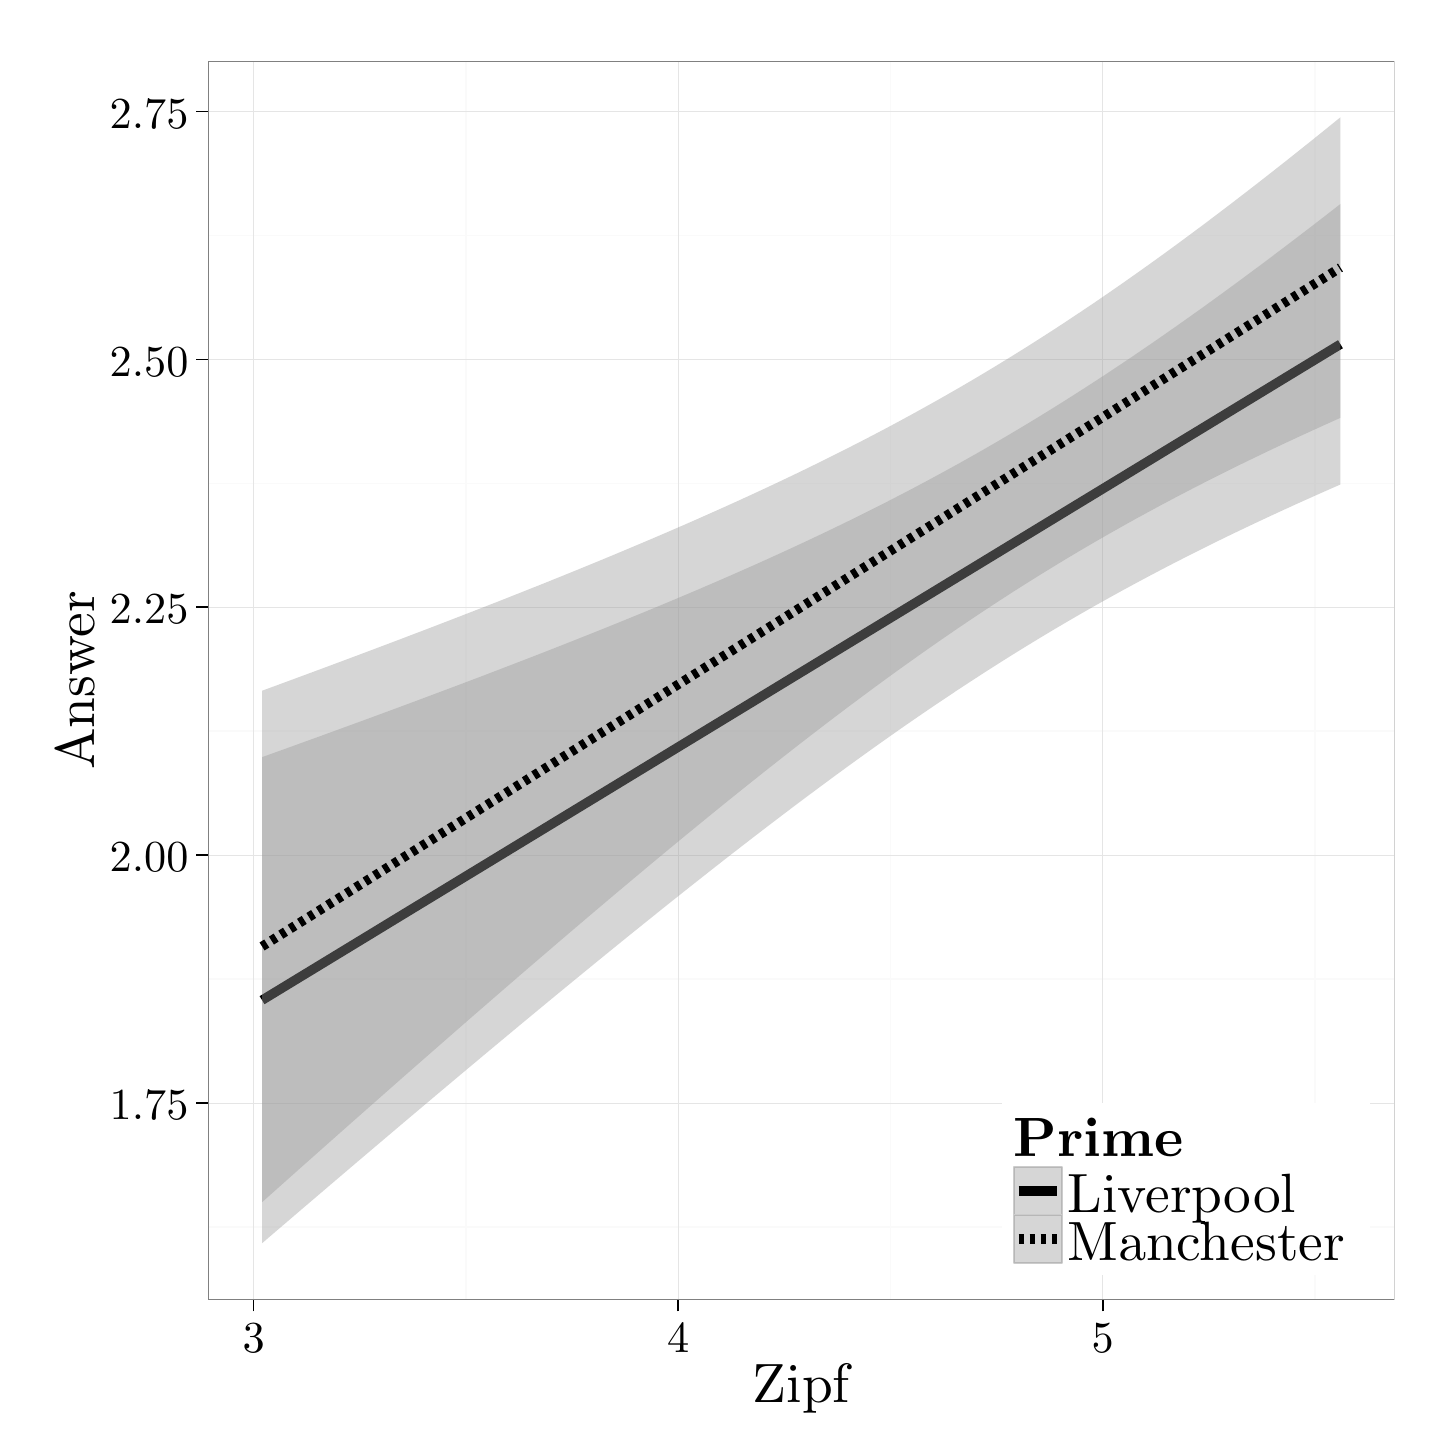
\begin{tikzpicture}[x=1pt,y=1pt]
\definecolor{fillColor}{RGB}{255,255,255}
\path[use as bounding box,fill=fillColor,fill opacity=0.00] (0,0) rectangle (505.89,505.89);
\begin{scope}
\path[clip] (  0.00,  0.00) rectangle (505.89,505.89);
\definecolor{drawColor}{RGB}{255,255,255}
\definecolor{fillColor}{RGB}{255,255,255}

\path[draw=drawColor,line width= 0.6pt,line join=round,line cap=round,fill=fillColor] (  0.00, -0.00) rectangle (505.89,505.89);
\end{scope}
\begin{scope}
\path[clip] ( 65.21, 46.31) rectangle (493.85,493.84);
\definecolor{fillColor}{RGB}{255,255,255}

\path[fill=fillColor] ( 65.21, 46.31) rectangle (493.85,493.84);
\definecolor{drawColor}{gray}{0.98}

\path[draw=drawColor,line width= 0.6pt,line join=round] ( 65.21, 72.56) --
	(493.85, 72.56);

\path[draw=drawColor,line width= 0.6pt,line join=round] ( 65.21,162.12) --
	(493.85,162.12);

\path[draw=drawColor,line width= 0.6pt,line join=round] ( 65.21,251.67) --
	(493.85,251.67);

\path[draw=drawColor,line width= 0.6pt,line join=round] ( 65.21,341.23) --
	(493.85,341.23);

\path[draw=drawColor,line width= 0.6pt,line join=round] ( 65.21,430.78) --
	(493.85,430.78);

\path[draw=drawColor,line width= 0.6pt,line join=round] (158.33, 46.31) --
	(158.33,493.84);

\path[draw=drawColor,line width= 0.6pt,line join=round] (311.75, 46.31) --
	(311.75,493.84);

\path[draw=drawColor,line width= 0.6pt,line join=round] (465.16, 46.31) --
	(465.16,493.84);
\definecolor{drawColor}{gray}{0.90}

\path[draw=drawColor,line width= 0.2pt,line join=round] ( 65.21,117.34) --
	(493.85,117.34);

\path[draw=drawColor,line width= 0.2pt,line join=round] ( 65.21,206.89) --
	(493.85,206.89);

\path[draw=drawColor,line width= 0.2pt,line join=round] ( 65.21,296.45) --
	(493.85,296.45);

\path[draw=drawColor,line width= 0.2pt,line join=round] ( 65.21,386.01) --
	(493.85,386.01);

\path[draw=drawColor,line width= 0.2pt,line join=round] ( 65.21,475.56) --
	(493.85,475.56);

\path[draw=drawColor,line width= 0.2pt,line join=round] ( 81.63, 46.31) --
	( 81.63,493.84);

\path[draw=drawColor,line width= 0.2pt,line join=round] (235.04, 46.31) --
	(235.04,493.84);

\path[draw=drawColor,line width= 0.2pt,line join=round] (388.45, 46.31) --
	(388.45,493.84);
\definecolor{fillColor}{RGB}{153,153,153}

\path[fill=fillColor,fill opacity=0.40] ( 84.70,242.29) --
	( 89.63,244.07) --
	( 94.56,245.84) --
	( 99.49,247.63) --
	(104.43,249.41) --
	(109.36,251.21) --
	(114.29,253.01) --
	(119.22,254.81) --
	(124.16,256.62) --
	(129.09,258.44) --
	(134.02,260.26) --
	(138.95,262.09) --
	(143.89,263.93) --
	(148.82,265.78) --
	(153.75,267.63) --
	(158.68,269.49) --
	(163.62,271.36) --
	(168.55,273.25) --
	(173.48,275.14) --
	(178.41,277.04) --
	(183.35,278.95) --
	(188.28,280.87) --
	(193.21,282.81) --
	(198.14,284.76) --
	(203.08,286.72) --
	(208.01,288.69) --
	(212.94,290.68) --
	(217.87,292.69) --
	(222.81,294.71) --
	(227.74,296.75) --
	(232.67,298.81) --
	(237.60,300.89) --
	(242.54,302.98) --
	(247.47,305.10) --
	(252.40,307.24) --
	(257.33,309.41) --
	(262.27,311.59) --
	(267.20,313.81) --
	(272.13,316.05) --
	(277.06,318.32) --
	(282.00,320.62) --
	(286.93,322.95) --
	(291.86,325.31) --
	(296.79,327.71) --
	(301.73,330.15) --
	(306.66,332.62) --
	(311.59,335.12) --
	(316.52,337.67) --
	(321.46,340.26) --
	(326.39,342.89) --
	(331.32,345.57) --
	(336.25,348.28) --
	(341.19,351.05) --
	(346.12,353.86) --
	(351.05,356.71) --
	(355.98,359.62) --
	(360.92,362.57) --
	(365.85,365.56) --
	(370.78,368.61) --
	(375.71,371.70) --
	(380.64,374.84) --
	(385.58,378.03) --
	(390.51,381.26) --
	(395.44,384.54) --
	(400.37,387.86) --
	(405.31,391.23) --
	(410.24,394.64) --
	(415.17,398.09) --
	(420.10,401.58) --
	(425.04,405.10) --
	(429.97,408.67) --
	(434.90,412.27) --
	(439.83,415.90) --
	(444.77,419.57) --
	(449.70,423.27) --
	(454.63,426.99) --
	(459.56,430.75) --
	(464.50,434.53) --
	(469.43,438.34) --
	(474.36,442.18) --
	(474.36,340.82) --
	(469.43,338.66) --
	(464.50,336.46) --
	(459.56,334.25) --
	(454.63,332.00) --
	(449.70,329.73) --
	(444.77,327.43) --
	(439.83,325.09) --
	(434.90,322.73) --
	(429.97,320.33) --
	(425.04,317.89) --
	(420.10,315.42) --
	(415.17,312.90) --
	(410.24,310.35) --
	(405.31,307.76) --
	(400.37,305.12) --
	(395.44,302.45) --
	(390.51,299.72) --
	(385.58,296.96) --
	(380.64,294.14) --
	(375.71,291.28) --
	(370.78,288.38) --
	(365.85,285.42) --
	(360.92,282.42) --
	(355.98,279.37) --
	(351.05,276.27) --
	(346.12,273.13) --
	(341.19,269.93) --
	(336.25,266.70) --
	(331.32,263.41) --
	(326.39,260.09) --
	(321.46,256.72) --
	(316.52,253.31) --
	(311.59,249.85) --
	(306.66,246.36) --
	(301.73,242.83) --
	(296.79,239.26) --
	(291.86,235.66) --
	(286.93,232.02) --
	(282.00,228.35) --
	(277.06,224.65) --
	(272.13,220.92) --
	(267.20,217.16) --
	(262.27,213.38) --
	(257.33,209.56) --
	(252.40,205.73) --
	(247.47,201.87) --
	(242.54,197.98) --
	(237.60,194.08) --
	(232.67,190.16) --
	(227.74,186.21) --
	(222.81,182.25) --
	(217.87,178.27) --
	(212.94,174.28) --
	(208.01,170.27) --
	(203.08,166.24) --
	(198.14,162.20) --
	(193.21,158.15) --
	(188.28,154.09) --
	(183.35,150.01) --
	(178.41,145.92) --
	(173.48,141.82) --
	(168.55,137.71) --
	(163.62,133.59) --
	(158.68,129.46) --
	(153.75,125.32) --
	(148.82,121.18) --
	(143.89,117.02) --
	(138.95,112.86) --
	(134.02,108.69) --
	(129.09,104.51) --
	(124.16,100.33) --
	(119.22, 96.14) --
	(114.29, 91.94) --
	(109.36, 87.74) --
	(104.43, 83.53) --
	( 99.49, 79.32) --
	( 94.56, 75.10) --
	( 89.63, 70.88) --
	( 84.70, 66.65) --
	cycle;
\definecolor{drawColor}{RGB}{0,0,0}

\path[draw=drawColor,line width= 3.4pt,line join=round] ( 84.70,154.47) --
	( 89.63,157.47) --
	( 94.56,160.47) --
	( 99.49,163.47) --
	(104.43,166.47) --
	(109.36,169.47) --
	(114.29,172.47) --
	(119.22,175.47) --
	(124.16,178.47) --
	(129.09,181.48) --
	(134.02,184.48) --
	(138.95,187.48) --
	(143.89,190.48) --
	(148.82,193.48) --
	(153.75,196.48) --
	(158.68,199.48) --
	(163.62,202.48) --
	(168.55,205.48) --
	(173.48,208.48) --
	(178.41,211.48) --
	(183.35,214.48) --
	(188.28,217.48) --
	(193.21,220.48) --
	(198.14,223.48) --
	(203.08,226.48) --
	(208.01,229.48) --
	(212.94,232.48) --
	(217.87,235.48) --
	(222.81,238.48) --
	(227.74,241.48) --
	(232.67,244.48) --
	(237.60,247.48) --
	(242.54,250.48) --
	(247.47,253.48) --
	(252.40,256.48) --
	(257.33,259.48) --
	(262.27,262.48) --
	(267.20,265.49) --
	(272.13,268.49) --
	(277.06,271.49) --
	(282.00,274.49) --
	(286.93,277.49) --
	(291.86,280.49) --
	(296.79,283.49) --
	(301.73,286.49) --
	(306.66,289.49) --
	(311.59,292.49) --
	(316.52,295.49) --
	(321.46,298.49) --
	(326.39,301.49) --
	(331.32,304.49) --
	(336.25,307.49) --
	(341.19,310.49) --
	(346.12,313.49) --
	(351.05,316.49) --
	(355.98,319.49) --
	(360.92,322.49) --
	(365.85,325.49) --
	(370.78,328.49) --
	(375.71,331.49) --
	(380.64,334.49) --
	(385.58,337.49) --
	(390.51,340.49) --
	(395.44,343.49) --
	(400.37,346.49) --
	(405.31,349.49) --
	(410.24,352.50) --
	(415.17,355.50) --
	(420.10,358.50) --
	(425.04,361.50) --
	(429.97,364.50) --
	(434.90,367.50) --
	(439.83,370.50) --
	(444.77,373.50) --
	(449.70,376.50) --
	(454.63,379.50) --
	(459.56,382.50) --
	(464.50,385.50) --
	(469.43,388.50) --
	(474.36,391.50);

\path[fill=fillColor,fill opacity=0.40] ( 84.70,266.29) --
	( 89.63,268.10) --
	( 94.56,269.92) --
	( 99.49,271.74) --
	(104.43,273.57) --
	(109.36,275.40) --
	(114.29,277.24) --
	(119.22,279.08) --
	(124.16,280.94) --
	(129.09,282.80) --
	(134.02,284.66) --
	(138.95,286.54) --
	(143.89,288.42) --
	(148.82,290.31) --
	(153.75,292.21) --
	(158.68,294.12) --
	(163.62,296.04) --
	(168.55,297.96) --
	(173.48,299.90) --
	(178.41,301.86) --
	(183.35,303.82) --
	(188.28,305.79) --
	(193.21,307.78) --
	(198.14,309.78) --
	(203.08,311.80) --
	(208.01,313.83) --
	(212.94,315.88) --
	(217.87,317.95) --
	(222.81,320.03) --
	(227.74,322.13) --
	(232.67,324.25) --
	(237.60,326.39) --
	(242.54,328.56) --
	(247.47,330.75) --
	(252.40,332.96) --
	(257.33,335.19) --
	(262.27,337.46) --
	(267.20,339.75) --
	(272.13,342.07) --
	(277.06,344.42) --
	(282.00,346.81) --
	(286.93,349.23) --
	(291.86,351.68) --
	(296.79,354.17) --
	(301.73,356.70) --
	(306.66,359.26) --
	(311.59,361.87) --
	(316.52,364.52) --
	(321.46,367.22) --
	(326.39,369.96) --
	(331.32,372.74) --
	(336.25,375.57) --
	(341.19,378.45) --
	(346.12,381.38) --
	(351.05,384.36) --
	(355.98,387.39) --
	(360.92,390.47) --
	(365.85,393.60) --
	(370.78,396.77) --
	(375.71,400.00) --
	(380.64,403.28) --
	(385.58,406.60) --
	(390.51,409.98) --
	(395.44,413.40) --
	(400.37,416.87) --
	(405.31,420.38) --
	(410.24,423.93) --
	(415.17,427.53) --
	(420.10,431.17) --
	(425.04,434.85) --
	(429.97,438.57) --
	(434.90,442.32) --
	(439.83,446.11) --
	(444.77,449.93) --
	(449.70,453.79) --
	(454.63,457.67) --
	(459.56,461.59) --
	(464.50,465.53) --
	(469.43,469.51) --
	(474.36,473.50) --
	(474.36,364.90) --
	(469.43,362.68) --
	(464.50,360.44) --
	(459.56,358.18) --
	(454.63,355.88) --
	(449.70,353.56) --
	(444.77,351.20) --
	(439.83,348.82) --
	(434.90,346.39) --
	(429.97,343.94) --
	(425.04,341.44) --
	(420.10,338.91) --
	(415.17,336.34) --
	(410.24,333.73) --
	(405.31,331.07) --
	(400.37,328.38) --
	(395.44,325.63) --
	(390.51,322.84) --
	(385.58,320.01) --
	(380.64,317.12) --
	(375.71,314.19) --
	(370.78,311.20) --
	(365.85,308.17) --
	(360.92,305.09) --
	(355.98,301.96) --
	(351.05,298.77) --
	(346.12,295.54) --
	(341.19,292.26) --
	(336.25,288.93) --
	(331.32,285.55) --
	(326.39,282.13) --
	(321.46,278.65) --
	(316.52,275.14) --
	(311.59,271.58) --
	(306.66,267.98) --
	(301.73,264.33) --
	(296.79,260.65) --
	(291.86,256.93) --
	(286.93,253.17) --
	(282.00,249.38) --
	(277.06,245.55) --
	(272.13,241.69) --
	(267.20,237.81) --
	(262.27,233.89) --
	(257.33,229.94) --
	(252.40,225.97) --
	(247.47,221.97) --
	(242.54,217.94) --
	(237.60,213.90) --
	(232.67,209.83) --
	(227.74,205.74) --
	(222.81,201.63) --
	(217.87,197.50) --
	(212.94,193.36) --
	(208.01,189.20) --
	(203.08,185.02) --
	(198.14,180.82) --
	(193.21,176.62) --
	(188.28,172.39) --
	(183.35,168.16) --
	(178.41,163.91) --
	(173.48,159.65) --
	(168.55,155.38) --
	(163.62,151.10) --
	(158.68,146.81) --
	(153.75,142.50) --
	(148.82,138.19) --
	(143.89,133.87) --
	(138.95,129.55) --
	(134.02,125.21) --
	(129.09,120.86) --
	(124.16,116.51) --
	(119.22,112.15) --
	(114.29,107.79) --
	(109.36,103.42) --
	(104.43, 99.04) --
	( 99.49, 94.66) --
	( 94.56, 90.27) --
	( 89.63, 85.87) --
	( 84.70, 81.47) --
	cycle;

\path[draw=drawColor,line width= 3.4pt,dash pattern=on 2pt off 2pt ,line join=round] ( 84.70,173.88) --
	( 89.63,176.99) --
	( 94.56,180.09) --
	( 99.49,183.20) --
	(104.43,186.30) --
	(109.36,189.41) --
	(114.29,192.51) --
	(119.22,195.62) --
	(124.16,198.72) --
	(129.09,201.83) --
	(134.02,204.94) --
	(138.95,208.04) --
	(143.89,211.15) --
	(148.82,214.25) --
	(153.75,217.36) --
	(158.68,220.46) --
	(163.62,223.57) --
	(168.55,226.67) --
	(173.48,229.78) --
	(178.41,232.88) --
	(183.35,235.99) --
	(188.28,239.09) --
	(193.21,242.20) --
	(198.14,245.30) --
	(203.08,248.41) --
	(208.01,251.51) --
	(212.94,254.62) --
	(217.87,257.73) --
	(222.81,260.83) --
	(227.74,263.94) --
	(232.67,267.04) --
	(237.60,270.15) --
	(242.54,273.25) --
	(247.47,276.36) --
	(252.40,279.46) --
	(257.33,282.57) --
	(262.27,285.67) --
	(267.20,288.78) --
	(272.13,291.88) --
	(277.06,294.99) --
	(282.00,298.09) --
	(286.93,301.20) --
	(291.86,304.30) --
	(296.79,307.41) --
	(301.73,310.51) --
	(306.66,313.62) --
	(311.59,316.73) --
	(316.52,319.83) --
	(321.46,322.94) --
	(326.39,326.04) --
	(331.32,329.15) --
	(336.25,332.25) --
	(341.19,335.36) --
	(346.12,338.46) --
	(351.05,341.57) --
	(355.98,344.67) --
	(360.92,347.78) --
	(365.85,350.88) --
	(370.78,353.99) --
	(375.71,357.09) --
	(380.64,360.20) --
	(385.58,363.30) --
	(390.51,366.41) --
	(395.44,369.52) --
	(400.37,372.62) --
	(405.31,375.73) --
	(410.24,378.83) --
	(415.17,381.94) --
	(420.10,385.04) --
	(425.04,388.15) --
	(429.97,391.25) --
	(434.90,394.36) --
	(439.83,397.46) --
	(444.77,400.57) --
	(449.70,403.67) --
	(454.63,406.78) --
	(459.56,409.88) --
	(464.50,412.99) --
	(469.43,416.09) --
	(474.36,419.20);
\definecolor{drawColor}{gray}{0.50}

\path[draw=drawColor,line width= 0.6pt,line join=round,line cap=round] ( 65.21, 46.31) rectangle (493.85,493.84);
\end{scope}
\begin{scope}
\path[clip] (  0.00,  0.00) rectangle (505.89,505.89);
\definecolor{drawColor}{RGB}{0,0,0}

\node[text=drawColor,anchor=base east,inner sep=0pt, outer sep=0pt, scale=  1.60] at ( 58.10,111.31) {1.75};

\node[text=drawColor,anchor=base east,inner sep=0pt, outer sep=0pt, scale=  1.60] at ( 58.10,200.86) {2.00};

\node[text=drawColor,anchor=base east,inner sep=0pt, outer sep=0pt, scale=  1.60] at ( 58.10,290.42) {2.25};

\node[text=drawColor,anchor=base east,inner sep=0pt, outer sep=0pt, scale=  1.60] at ( 58.10,379.97) {2.50};

\node[text=drawColor,anchor=base east,inner sep=0pt, outer sep=0pt, scale=  1.60] at ( 58.10,469.53) {2.75};
\end{scope}
\begin{scope}
\path[clip] (  0.00,  0.00) rectangle (505.89,505.89);
\definecolor{drawColor}{RGB}{0,0,0}

\path[draw=drawColor,line width= 0.6pt,line join=round] ( 60.95,117.34) --
	( 65.21,117.34);

\path[draw=drawColor,line width= 0.6pt,line join=round] ( 60.95,206.89) --
	( 65.21,206.89);

\path[draw=drawColor,line width= 0.6pt,line join=round] ( 60.95,296.45) --
	( 65.21,296.45);

\path[draw=drawColor,line width= 0.6pt,line join=round] ( 60.95,386.01) --
	( 65.21,386.01);

\path[draw=drawColor,line width= 0.6pt,line join=round] ( 60.95,475.56) --
	( 65.21,475.56);
\end{scope}
\begin{scope}
\path[clip] (  0.00,  0.00) rectangle (505.89,505.89);
\definecolor{drawColor}{RGB}{0,0,0}

\path[draw=drawColor,line width= 0.6pt,line join=round] ( 81.63, 42.04) --
	( 81.63, 46.31);

\path[draw=drawColor,line width= 0.6pt,line join=round] (235.04, 42.04) --
	(235.04, 46.31);

\path[draw=drawColor,line width= 0.6pt,line join=round] (388.45, 42.04) --
	(388.45, 46.31);
\end{scope}
\begin{scope}
\path[clip] (  0.00,  0.00) rectangle (505.89,505.89);
\definecolor{drawColor}{RGB}{0,0,0}

\node[text=drawColor,anchor=base,inner sep=0pt, outer sep=0pt, scale=  1.60] at ( 81.63, 27.13) {3};

\node[text=drawColor,anchor=base,inner sep=0pt, outer sep=0pt, scale=  1.60] at (235.04, 27.13) {4};

\node[text=drawColor,anchor=base,inner sep=0pt, outer sep=0pt, scale=  1.60] at (388.45, 27.13) {5};
\end{scope}
\begin{scope}
\path[clip] (  0.00,  0.00) rectangle (505.89,505.89);
\definecolor{drawColor}{RGB}{0,0,0}

\node[text=drawColor,anchor=base,inner sep=0pt, outer sep=0pt, scale=  2.00] at (279.53,  9.03) {Zipf};
\end{scope}
\begin{scope}
\path[clip] (  0.00,  0.00) rectangle (505.89,505.89);
\definecolor{drawColor}{RGB}{0,0,0}

\node[text=drawColor,rotate= 90.00,anchor=base,inner sep=0pt, outer sep=0pt, scale=  2.00] at ( 24.12,270.08) {Answer};
\end{scope}
\begin{scope}
\path[clip] (  0.00,  0.00) rectangle (505.89,505.89);
\definecolor{fillColor}{RGB}{255,255,255}

\path[fill=fillColor] (352.06, 55.18) rectangle (484.98,117.15);
\end{scope}
\begin{scope}
\path[clip] (  0.00,  0.00) rectangle (505.89,505.89);
\definecolor{drawColor}{RGB}{0,0,0}

\node[text=drawColor,anchor=base west,inner sep=0pt, outer sep=0pt, scale=  2.00] at (356.32, 98.13) {\bfseries Prime};
\end{scope}
\begin{scope}
\path[clip] (  0.00,  0.00) rectangle (505.89,505.89);
\definecolor{drawColor}{gray}{0.80}
\definecolor{fillColor}{RGB}{255,255,255}

\path[draw=drawColor,line width= 0.6pt,line join=round,line cap=round,fill=fillColor] (356.32, 76.79) rectangle (373.67, 94.13);
\end{scope}
\begin{scope}
\path[clip] (  0.00,  0.00) rectangle (505.89,505.89);
\definecolor{fillColor}{RGB}{153,153,153}

\path[fill=fillColor,fill opacity=0.40] (356.32, 76.79) rectangle (373.67, 94.13);
\definecolor{drawColor}{RGB}{0,0,0}

\path[draw=drawColor,line width= 3.4pt,line join=round] (358.06, 85.46) -- (371.93, 85.46);
\end{scope}
\begin{scope}
\path[clip] (  0.00,  0.00) rectangle (505.89,505.89);
\definecolor{drawColor}{gray}{0.80}
\definecolor{fillColor}{RGB}{255,255,255}

\path[draw=drawColor,line width= 0.6pt,line join=round,line cap=round,fill=fillColor] (356.32, 59.44) rectangle (373.67, 76.79);
\end{scope}
\begin{scope}
\path[clip] (  0.00,  0.00) rectangle (505.89,505.89);
\definecolor{fillColor}{RGB}{153,153,153}

\path[fill=fillColor,fill opacity=0.40] (356.32, 59.44) rectangle (373.67, 76.79);
\definecolor{drawColor}{RGB}{0,0,0}

\path[draw=drawColor,line width= 3.4pt,dash pattern=on 2pt off 2pt ,line join=round] (358.06, 68.12) -- (371.93, 68.12);
\end{scope}
\begin{scope}
\path[clip] (  0.00,  0.00) rectangle (505.89,505.89);
\definecolor{drawColor}{RGB}{0,0,0}

\node[text=drawColor,anchor=base west,inner sep=0pt, outer sep=0pt, scale=  2.00] at (375.84, 77.92) {Liverpool};
\end{scope}
\begin{scope}
\path[clip] (  0.00,  0.00) rectangle (505.89,505.89);
\definecolor{drawColor}{RGB}{0,0,0}

\node[text=drawColor,anchor=base west,inner sep=0pt, outer sep=0pt, scale=  2.00] at (375.84, 60.57) {Manchester};
\end{scope}
\end{tikzpicture}
} 
	\caption{happ\textsc{y} (perception) by Zipf score}
	\label{fig.scatter.happy.ext.zipf}
\end{figure}

For the sake of completeness we will now briefly turn to frequency and age because these two factors show up as (near-)significant in a mixed-effects model that includes the \isi{Zipf} scores (see page \pageref{sec.perc_res.happy}).
The coefficient for the factor frequency of the carrier word (0.622) is positive in the model not reported here, which means that for higher frequency carrier words higher-numbered (i.e. more Liverpool-like) answer options were more likely.
This general correlation is visible in Figure \ref{fig.scatter.happy.ext.zipf}, which shows \isi{Zipf} scores on the x-axis and estimated \isi{percept} on the y-axis; \isi{priming} condition is again shown by line type (solid for \isi{Liverpool}, dashed for \isi{Manchester}).
We can see the positive correlation suggested by the linear mixed-effects model: more centralised percepts for lower frequency items (on the left) and tenser percepts for higher frequency items (on the right).
It should be borne in mind, however, that we are only looking at a very restricted set of 6 different carrier words, so the potential frequency effect we are seeing could be heavily overlaid with \emph{lexical} effects, although the two are not unlikely to interact anyway.
The direct cause for the correlation of frequency and reported \isi{percept} might quite simply be that the higher frequency carrier words are realised with tenser happ\textsc{y} in the particular stimuli used for this study.
There is indeed a trend of this sort in the data: higher-frequency words in the stimuli sentence have a slightly lower F1 and simultaneously a higher F2, the difference between the most frequent and the least frequent two carrier words is about 100 Hz for F1 and about 80 Hz for F2.
However, this difference is then carried into the answer tokens since they were generated individually for each sentence (cf. \ref{sec.perc_method.sentences} and \ref{sec.perc_method.vow}), so the effect cannot really be due to the test material.
The most important point, in any case, is that, again, the figure supports the absence of a \isi{prime} X \isi{Zipf} score interaction in the mixed-effects ordinal regression model.
While there are smaller differences between \isi{priming} conditions, the general relationship between reported \isi{percept} and \isi{Zipf} score seems to be the same regardless of whether participants believe they are listening to a speaker from \isi{Liverpool} or \isi{Manchester}.
Both the solid and the dashed regression line have an upward slope that is almost identical (the lines are very nearly parallel), which illustrates that the effect of frequency (if there is any) is the same in both \isi{priming} conditions.

\subsection{Age}
\label{sec.perc_res.happy.age}

\begin{figure}[h]
	\centering
		\definecolor{shadecolor}{rgb}{0.969, 0.969, 0.969}
		\resizebox{.49\linewidth}{!}{% Created by tikzDevice version 0.8.1 on 2016-02-09 02:18:30
% !TEX encoding = UTF-8 Unicode
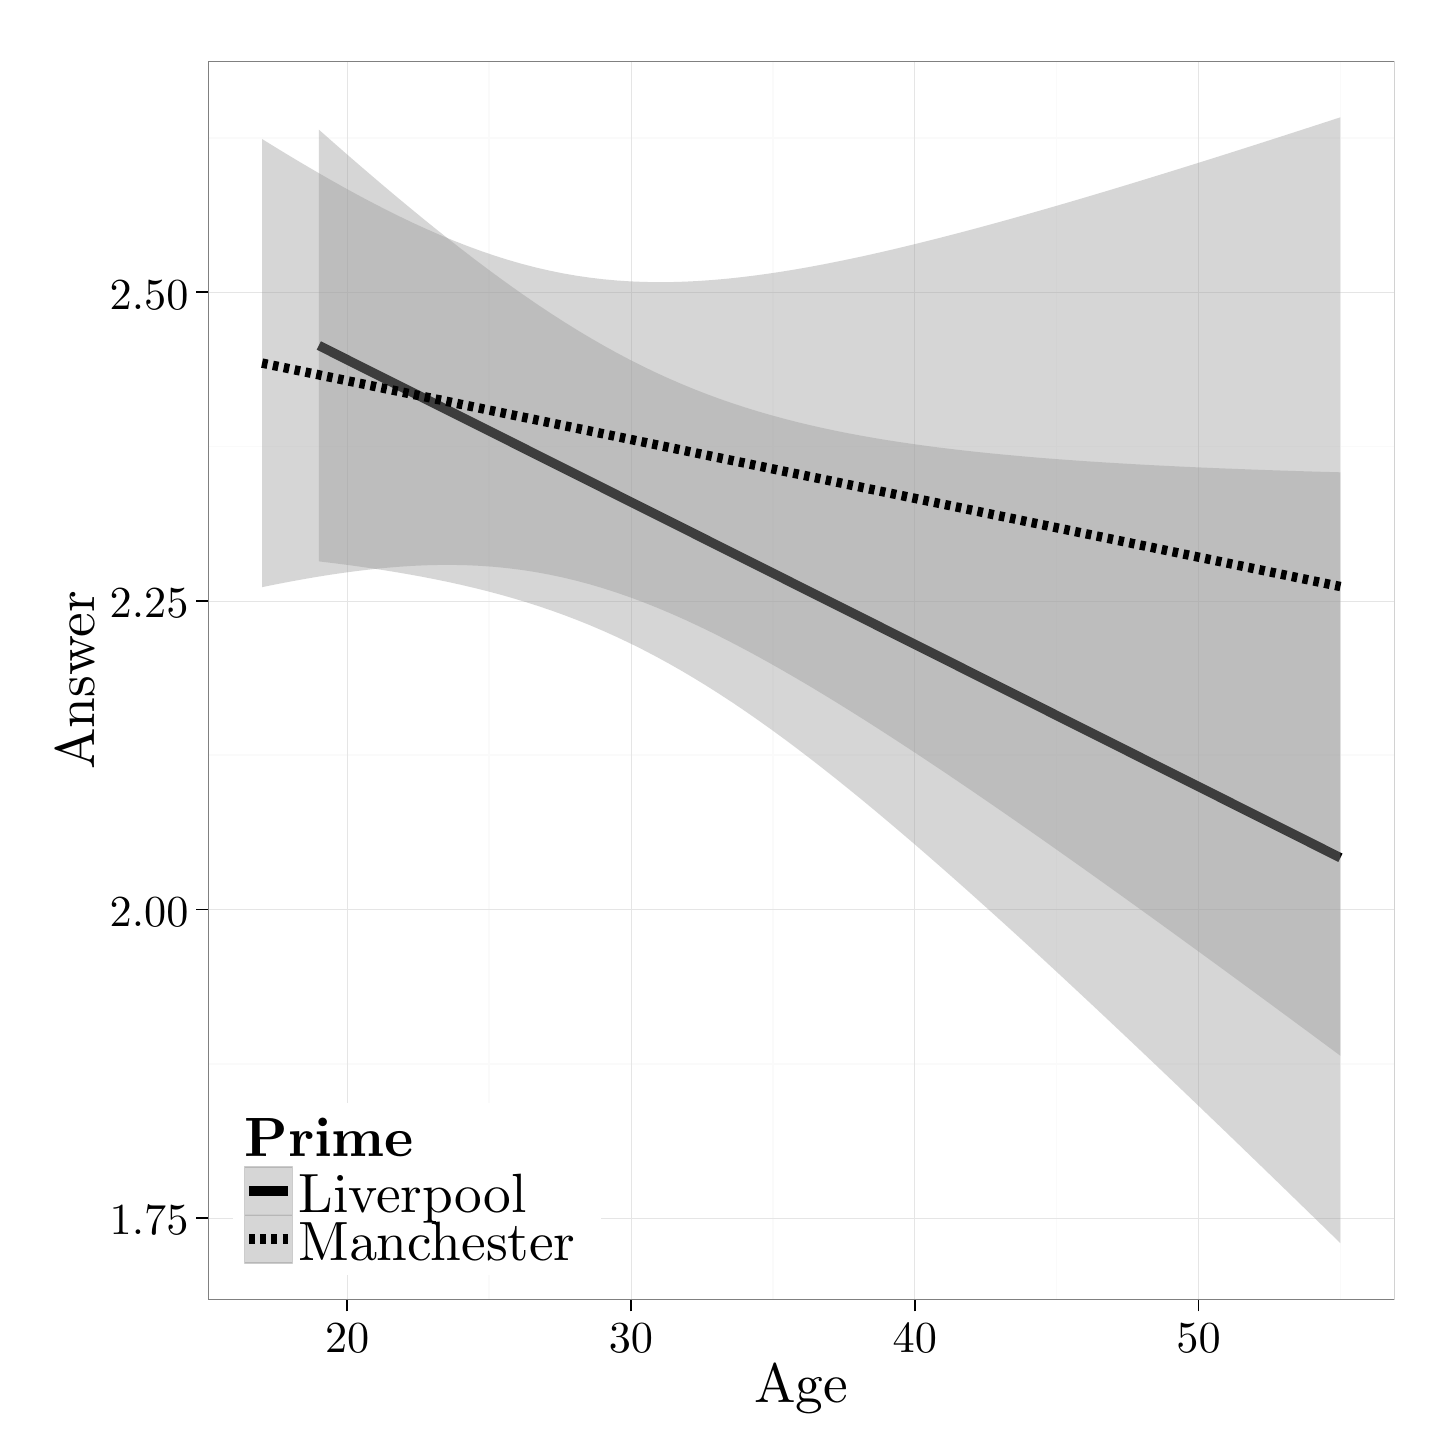
\begin{tikzpicture}[x=1pt,y=1pt]
\definecolor{fillColor}{RGB}{255,255,255}
\path[use as bounding box,fill=fillColor,fill opacity=0.00] (0,0) rectangle (505.89,505.89);
\begin{scope}
\path[clip] (  0.00,  0.00) rectangle (505.89,505.89);
\definecolor{drawColor}{RGB}{255,255,255}
\definecolor{fillColor}{RGB}{255,255,255}

\path[draw=drawColor,line width= 0.6pt,line join=round,line cap=round,fill=fillColor] (  0.00, -0.00) rectangle (505.89,505.89);
\end{scope}
\begin{scope}
\path[clip] ( 65.21, 46.31) rectangle (493.85,493.84);
\definecolor{fillColor}{RGB}{255,255,255}

\path[fill=fillColor] ( 65.21, 46.31) rectangle (493.85,493.84);
\definecolor{drawColor}{gray}{0.98}

\path[draw=drawColor,line width= 0.6pt,line join=round] ( 65.21,131.45) --
	(493.85,131.45);

\path[draw=drawColor,line width= 0.6pt,line join=round] ( 65.21,242.97) --
	(493.85,242.97);

\path[draw=drawColor,line width= 0.6pt,line join=round] ( 65.21,354.50) --
	(493.85,354.50);

\path[draw=drawColor,line width= 0.6pt,line join=round] ( 65.21,466.02) --
	(493.85,466.02);

\path[draw=drawColor,line width= 0.6pt,line join=round] (166.73, 46.31) --
	(166.73,493.84);

\path[draw=drawColor,line width= 0.6pt,line join=round] (269.28, 46.31) --
	(269.28,493.84);

\path[draw=drawColor,line width= 0.6pt,line join=round] (371.82, 46.31) --
	(371.82,493.84);

\path[draw=drawColor,line width= 0.6pt,line join=round] (474.36, 46.31) --
	(474.36,493.84);
\definecolor{drawColor}{gray}{0.90}

\path[draw=drawColor,line width= 0.2pt,line join=round] ( 65.21, 75.68) --
	(493.85, 75.68);

\path[draw=drawColor,line width= 0.2pt,line join=round] ( 65.21,187.21) --
	(493.85,187.21);

\path[draw=drawColor,line width= 0.2pt,line join=round] ( 65.21,298.73) --
	(493.85,298.73);

\path[draw=drawColor,line width= 0.2pt,line join=round] ( 65.21,410.26) --
	(493.85,410.26);

\path[draw=drawColor,line width= 0.2pt,line join=round] (115.46, 46.31) --
	(115.46,493.84);

\path[draw=drawColor,line width= 0.2pt,line join=round] (218.00, 46.31) --
	(218.00,493.84);

\path[draw=drawColor,line width= 0.2pt,line join=round] (320.55, 46.31) --
	(320.55,493.84);

\path[draw=drawColor,line width= 0.2pt,line join=round] (423.09, 46.31) --
	(423.09,493.84);
\definecolor{fillColor}{RGB}{153,153,153}

\path[fill=fillColor,fill opacity=0.40] (105.21,469.04) --
	(109.88,464.92) --
	(114.55,460.82) --
	(119.22,456.77) --
	(123.90,452.75) --
	(128.57,448.77) --
	(133.24,444.84) --
	(137.92,440.96) --
	(142.59,437.12) --
	(147.26,433.34) --
	(151.93,429.62) --
	(156.61,425.97) --
	(161.28,422.38) --
	(165.95,418.86) --
	(170.63,415.41) --
	(175.30,412.05) --
	(179.97,408.77) --
	(184.64,405.57) --
	(189.32,402.47) --
	(193.99,399.47) --
	(198.66,396.57) --
	(203.34,393.77) --
	(208.01,391.08) --
	(212.68,388.49) --
	(217.35,386.02) --
	(222.03,383.66) --
	(226.70,381.40) --
	(231.37,379.26) --
	(236.05,377.23) --
	(240.72,375.30) --
	(245.39,373.48) --
	(250.06,371.76) --
	(254.74,370.14) --
	(259.41,368.62) --
	(264.08,367.18) --
	(268.76,365.83) --
	(273.43,364.56) --
	(278.10,363.36) --
	(282.77,362.24) --
	(287.45,361.19) --
	(292.12,360.20) --
	(296.79,359.27) --
	(301.47,358.40) --
	(306.14,357.58) --
	(310.81,356.81) --
	(315.48,356.09) --
	(320.16,355.40) --
	(324.83,354.76) --
	(329.50,354.15) --
	(334.18,353.58) --
	(338.85,353.04) --
	(343.52,352.53) --
	(348.19,352.05) --
	(352.87,351.60) --
	(357.54,351.17) --
	(362.21,350.76) --
	(366.89,350.37) --
	(371.56,350.01) --
	(376.23,349.66) --
	(380.90,349.33) --
	(385.58,349.02) --
	(390.25,348.72) --
	(394.92,348.44) --
	(399.60,348.17) --
	(404.27,347.91) --
	(408.94,347.67) --
	(413.61,347.44) --
	(418.29,347.21) --
	(422.96,347.00) --
	(427.63,346.80) --
	(432.31,346.61) --
	(436.98,346.43) --
	(441.65,346.25) --
	(446.32,346.08) --
	(451.00,345.92) --
	(455.67,345.77) --
	(460.34,345.62) --
	(465.02,345.48) --
	(469.69,345.35) --
	(474.36,345.22) --
	(474.36, 66.65) --
	(469.69, 71.21) --
	(465.02, 75.76) --
	(460.34, 80.31) --
	(455.67, 84.85) --
	(451.00, 89.38) --
	(446.32, 93.91) --
	(441.65, 98.42) --
	(436.98,102.94) --
	(432.31,107.44) --
	(427.63,111.93) --
	(422.96,116.42) --
	(418.29,120.89) --
	(413.61,125.36) --
	(408.94,129.81) --
	(404.27,134.25) --
	(399.60,138.68) --
	(394.92,143.10) --
	(390.25,147.50) --
	(385.58,151.89) --
	(380.90,156.26) --
	(376.23,160.62) --
	(371.56,164.96) --
	(366.89,169.28) --
	(362.21,173.58) --
	(357.54,177.86) --
	(352.87,182.11) --
	(348.19,186.34) --
	(343.52,190.55) --
	(338.85,194.73) --
	(334.18,198.87) --
	(329.50,202.99) --
	(324.83,207.07) --
	(320.16,211.11) --
	(315.48,215.11) --
	(310.81,219.07) --
	(306.14,222.99) --
	(301.47,226.86) --
	(296.79,230.67) --
	(292.12,234.43) --
	(287.45,238.12) --
	(282.77,241.76) --
	(278.10,245.32) --
	(273.43,248.82) --
	(268.76,252.23) --
	(264.08,255.57) --
	(259.41,258.82) --
	(254.74,261.98) --
	(250.06,265.04) --
	(245.39,268.01) --
	(240.72,270.87) --
	(236.05,273.63) --
	(231.37,276.29) --
	(226.70,278.83) --
	(222.03,281.27) --
	(217.35,283.59) --
	(212.68,285.80) --
	(208.01,287.90) --
	(203.34,289.90) --
	(198.66,291.78) --
	(193.99,293.57) --
	(189.32,295.25) --
	(184.64,296.84) --
	(179.97,298.33) --
	(175.30,299.74) --
	(170.63,301.06) --
	(165.95,302.30) --
	(161.28,303.46) --
	(156.61,304.56) --
	(151.93,305.59) --
	(147.26,306.55) --
	(142.59,307.46) --
	(137.92,308.31) --
	(133.24,309.12) --
	(128.57,309.87) --
	(123.90,310.58) --
	(119.22,311.25) --
	(114.55,311.88) --
	(109.88,312.47) --
	(105.21,313.03) --
	cycle;
\definecolor{drawColor}{RGB}{0,0,0}

\path[draw=drawColor,line width= 3.4pt,line join=round] (105.21,391.04) --
	(109.88,388.69) --
	(114.55,386.35) --
	(119.22,384.01) --
	(123.90,381.66) --
	(128.57,379.32) --
	(133.24,376.98) --
	(137.92,374.64) --
	(142.59,372.29) --
	(147.26,369.95) --
	(151.93,367.61) --
	(156.61,365.26) --
	(161.28,362.92) --
	(165.95,360.58) --
	(170.63,358.23) --
	(175.30,355.89) --
	(179.97,353.55) --
	(184.64,351.20) --
	(189.32,348.86) --
	(193.99,346.52) --
	(198.66,344.18) --
	(203.34,341.83) --
	(208.01,339.49) --
	(212.68,337.15) --
	(217.35,334.80) --
	(222.03,332.46) --
	(226.70,330.12) --
	(231.37,327.77) --
	(236.05,325.43) --
	(240.72,323.09) --
	(245.39,320.75) --
	(250.06,318.40) --
	(254.74,316.06) --
	(259.41,313.72) --
	(264.08,311.37) --
	(268.76,309.03) --
	(273.43,306.69) --
	(278.10,304.34) --
	(282.77,302.00) --
	(287.45,299.66) --
	(292.12,297.31) --
	(296.79,294.97) --
	(301.47,292.63) --
	(306.14,290.29) --
	(310.81,287.94) --
	(315.48,285.60) --
	(320.16,283.26) --
	(324.83,280.91) --
	(329.50,278.57) --
	(334.18,276.23) --
	(338.85,273.88) --
	(343.52,271.54) --
	(348.19,269.20) --
	(352.87,266.86) --
	(357.54,264.51) --
	(362.21,262.17) --
	(366.89,259.83) --
	(371.56,257.48) --
	(376.23,255.14) --
	(380.90,252.80) --
	(385.58,250.45) --
	(390.25,248.11) --
	(394.92,245.77) --
	(399.60,243.42) --
	(404.27,241.08) --
	(408.94,238.74) --
	(413.61,236.40) --
	(418.29,234.05) --
	(422.96,231.71) --
	(427.63,229.37) --
	(432.31,227.02) --
	(436.98,224.68) --
	(441.65,222.34) --
	(446.32,219.99) --
	(451.00,217.65) --
	(455.67,215.31) --
	(460.34,212.97) --
	(465.02,210.62) --
	(469.69,208.28) --
	(474.36,205.94);

\path[fill=fillColor,fill opacity=0.40] ( 84.70,465.65) --
	( 89.63,462.60) --
	( 94.56,459.60) --
	( 99.49,456.66) --
	(104.43,453.77) --
	(109.36,450.94) --
	(114.29,448.17) --
	(119.22,445.47) --
	(124.16,442.85) --
	(129.09,440.31) --
	(134.02,437.85) --
	(138.95,435.48) --
	(143.89,433.22) --
	(148.82,431.05) --
	(153.75,429.00) --
	(158.68,427.06) --
	(163.62,425.25) --
	(168.55,423.56) --
	(173.48,422.00) --
	(178.41,420.58) --
	(183.35,419.29) --
	(188.28,418.15) --
	(193.21,417.14) --
	(198.14,416.28) --
	(203.08,415.56) --
	(208.01,414.97) --
	(212.94,414.52) --
	(217.87,414.20) --
	(222.81,414.00) --
	(227.74,413.93) --
	(232.67,413.96) --
	(237.60,414.11) --
	(242.54,414.36) --
	(247.47,414.71) --
	(252.40,415.14) --
	(257.33,415.66) --
	(262.27,416.26) --
	(267.20,416.93) --
	(272.13,417.67) --
	(277.06,418.47) --
	(282.00,419.33) --
	(286.93,420.25) --
	(291.86,421.22) --
	(296.79,422.23) --
	(301.73,423.28) --
	(306.66,424.38) --
	(311.59,425.51) --
	(316.52,426.68) --
	(321.46,427.88) --
	(326.39,429.11) --
	(331.32,430.37) --
	(336.25,431.65) --
	(341.19,432.95) --
	(346.12,434.28) --
	(351.05,435.63) --
	(355.98,437.00) --
	(360.92,438.39) --
	(365.85,439.80) --
	(370.78,441.22) --
	(375.71,442.65) --
	(380.64,444.10) --
	(385.58,445.57) --
	(390.51,447.04) --
	(395.44,448.53) --
	(400.37,450.03) --
	(405.31,451.54) --
	(410.24,453.06) --
	(415.17,454.59) --
	(420.10,456.12) --
	(425.04,457.67) --
	(429.97,459.22) --
	(434.90,460.78) --
	(439.83,462.35) --
	(444.77,463.93) --
	(449.70,465.51) --
	(454.63,467.10) --
	(459.56,468.69) --
	(464.50,470.29) --
	(469.43,471.89) --
	(474.36,473.50) --
	(474.36,134.38) --
	(469.43,138.03) --
	(464.50,141.68) --
	(459.56,145.32) --
	(454.63,148.96) --
	(449.70,152.59) --
	(444.77,156.22) --
	(439.83,159.84) --
	(434.90,163.45) --
	(429.97,167.06) --
	(425.04,170.65) --
	(420.10,174.24) --
	(415.17,177.82) --
	(410.24,181.40) --
	(405.31,184.96) --
	(400.37,188.51) --
	(395.44,192.06) --
	(390.51,195.59) --
	(385.58,199.11) --
	(380.64,202.62) --
	(375.71,206.11) --
	(370.78,209.59) --
	(365.85,213.06) --
	(360.92,216.50) --
	(355.98,219.94) --
	(351.05,223.35) --
	(346.12,226.74) --
	(341.19,230.12) --
	(336.25,233.47) --
	(331.32,236.80) --
	(326.39,240.10) --
	(321.46,243.37) --
	(316.52,246.61) --
	(311.59,249.82) --
	(306.66,253.00) --
	(301.73,256.14) --
	(296.79,259.24) --
	(291.86,262.30) --
	(286.93,265.31) --
	(282.00,268.27) --
	(277.06,271.17) --
	(272.13,274.02) --
	(267.20,276.80) --
	(262.27,279.52) --
	(257.33,282.16) --
	(252.40,284.72) --
	(247.47,287.20) --
	(242.54,289.59) --
	(237.60,291.89) --
	(232.67,294.08) --
	(227.74,296.16) --
	(222.81,298.13) --
	(217.87,299.98) --
	(212.94,301.70) --
	(208.01,303.29) --
	(203.08,304.75) --
	(198.14,306.07) --
	(193.21,307.25) --
	(188.28,308.29) --
	(183.35,309.19) --
	(178.41,309.95) --
	(173.48,310.57) --
	(168.55,311.06) --
	(163.62,311.41) --
	(158.68,311.64) --
	(153.75,311.75) --
	(148.82,311.74) --
	(143.89,311.62) --
	(138.95,311.40) --
	(134.02,311.07) --
	(129.09,310.66) --
	(124.16,310.16) --
	(119.22,309.58) --
	(114.29,308.93) --
	(109.36,308.21) --
	(104.43,307.42) --
	( 99.49,306.57) --
	( 94.56,305.67) --
	( 89.63,304.72) --
	( 84.70,303.72) --
	cycle;

\path[draw=drawColor,line width= 3.4pt,dash pattern=on 2pt off 2pt ,line join=round] ( 84.70,384.68) --
	( 89.63,383.66) --
	( 94.56,382.64) --
	( 99.49,381.62) --
	(104.43,380.59) --
	(109.36,379.57) --
	(114.29,378.55) --
	(119.22,377.53) --
	(124.16,376.51) --
	(129.09,375.48) --
	(134.02,374.46) --
	(138.95,373.44) --
	(143.89,372.42) --
	(148.82,371.40) --
	(153.75,370.37) --
	(158.68,369.35) --
	(163.62,368.33) --
	(168.55,367.31) --
	(173.48,366.29) --
	(178.41,365.26) --
	(183.35,364.24) --
	(188.28,363.22) --
	(193.21,362.20) --
	(198.14,361.18) --
	(203.08,360.15) --
	(208.01,359.13) --
	(212.94,358.11) --
	(217.87,357.09) --
	(222.81,356.07) --
	(227.74,355.04) --
	(232.67,354.02) --
	(237.60,353.00) --
	(242.54,351.98) --
	(247.47,350.95) --
	(252.40,349.93) --
	(257.33,348.91) --
	(262.27,347.89) --
	(267.20,346.87) --
	(272.13,345.84) --
	(277.06,344.82) --
	(282.00,343.80) --
	(286.93,342.78) --
	(291.86,341.76) --
	(296.79,340.73) --
	(301.73,339.71) --
	(306.66,338.69) --
	(311.59,337.67) --
	(316.52,336.65) --
	(321.46,335.62) --
	(326.39,334.60) --
	(331.32,333.58) --
	(336.25,332.56) --
	(341.19,331.54) --
	(346.12,330.51) --
	(351.05,329.49) --
	(355.98,328.47) --
	(360.92,327.45) --
	(365.85,326.43) --
	(370.78,325.40) --
	(375.71,324.38) --
	(380.64,323.36) --
	(385.58,322.34) --
	(390.51,321.32) --
	(395.44,320.29) --
	(400.37,319.27) --
	(405.31,318.25) --
	(410.24,317.23) --
	(415.17,316.21) --
	(420.10,315.18) --
	(425.04,314.16) --
	(429.97,313.14) --
	(434.90,312.12) --
	(439.83,311.10) --
	(444.77,310.07) --
	(449.70,309.05) --
	(454.63,308.03) --
	(459.56,307.01) --
	(464.50,305.99) --
	(469.43,304.96) --
	(474.36,303.94);
\definecolor{drawColor}{gray}{0.50}

\path[draw=drawColor,line width= 0.6pt,line join=round,line cap=round] ( 65.21, 46.31) rectangle (493.85,493.84);
\end{scope}
\begin{scope}
\path[clip] (  0.00,  0.00) rectangle (505.89,505.89);
\definecolor{drawColor}{RGB}{0,0,0}

\node[text=drawColor,anchor=base east,inner sep=0pt, outer sep=0pt, scale=  1.60] at ( 58.10, 69.65) {1.75};

\node[text=drawColor,anchor=base east,inner sep=0pt, outer sep=0pt, scale=  1.60] at ( 58.10,181.18) {2.00};

\node[text=drawColor,anchor=base east,inner sep=0pt, outer sep=0pt, scale=  1.60] at ( 58.10,292.70) {2.25};

\node[text=drawColor,anchor=base east,inner sep=0pt, outer sep=0pt, scale=  1.60] at ( 58.10,404.23) {2.50};
\end{scope}
\begin{scope}
\path[clip] (  0.00,  0.00) rectangle (505.89,505.89);
\definecolor{drawColor}{RGB}{0,0,0}

\path[draw=drawColor,line width= 0.6pt,line join=round] ( 60.95, 75.68) --
	( 65.21, 75.68);

\path[draw=drawColor,line width= 0.6pt,line join=round] ( 60.95,187.21) --
	( 65.21,187.21);

\path[draw=drawColor,line width= 0.6pt,line join=round] ( 60.95,298.73) --
	( 65.21,298.73);

\path[draw=drawColor,line width= 0.6pt,line join=round] ( 60.95,410.26) --
	( 65.21,410.26);
\end{scope}
\begin{scope}
\path[clip] (  0.00,  0.00) rectangle (505.89,505.89);
\definecolor{drawColor}{RGB}{0,0,0}

\path[draw=drawColor,line width= 0.6pt,line join=round] (115.46, 42.04) --
	(115.46, 46.31);

\path[draw=drawColor,line width= 0.6pt,line join=round] (218.00, 42.04) --
	(218.00, 46.31);

\path[draw=drawColor,line width= 0.6pt,line join=round] (320.55, 42.04) --
	(320.55, 46.31);

\path[draw=drawColor,line width= 0.6pt,line join=round] (423.09, 42.04) --
	(423.09, 46.31);
\end{scope}
\begin{scope}
\path[clip] (  0.00,  0.00) rectangle (505.89,505.89);
\definecolor{drawColor}{RGB}{0,0,0}

\node[text=drawColor,anchor=base,inner sep=0pt, outer sep=0pt, scale=  1.60] at (115.46, 27.13) {20};

\node[text=drawColor,anchor=base,inner sep=0pt, outer sep=0pt, scale=  1.60] at (218.00, 27.13) {30};

\node[text=drawColor,anchor=base,inner sep=0pt, outer sep=0pt, scale=  1.60] at (320.55, 27.13) {40};

\node[text=drawColor,anchor=base,inner sep=0pt, outer sep=0pt, scale=  1.60] at (423.09, 27.13) {50};
\end{scope}
\begin{scope}
\path[clip] (  0.00,  0.00) rectangle (505.89,505.89);
\definecolor{drawColor}{RGB}{0,0,0}

\node[text=drawColor,anchor=base,inner sep=0pt, outer sep=0pt, scale=  2.00] at (279.53,  9.03) {Age};
\end{scope}
\begin{scope}
\path[clip] (  0.00,  0.00) rectangle (505.89,505.89);
\definecolor{drawColor}{RGB}{0,0,0}

\node[text=drawColor,rotate= 90.00,anchor=base,inner sep=0pt, outer sep=0pt, scale=  2.00] at ( 24.12,270.08) {Answer};
\end{scope}
\begin{scope}
\path[clip] (  0.00,  0.00) rectangle (505.89,505.89);
\definecolor{fillColor}{RGB}{255,255,255}

\path[fill=fillColor] ( 74.08, 55.18) rectangle (207.00,117.15);
\end{scope}
\begin{scope}
\path[clip] (  0.00,  0.00) rectangle (505.89,505.89);
\definecolor{drawColor}{RGB}{0,0,0}

\node[text=drawColor,anchor=base west,inner sep=0pt, outer sep=0pt, scale=  2.00] at ( 78.35, 98.13) {\bfseries Prime};
\end{scope}
\begin{scope}
\path[clip] (  0.00,  0.00) rectangle (505.89,505.89);
\definecolor{drawColor}{gray}{0.80}
\definecolor{fillColor}{RGB}{255,255,255}

\path[draw=drawColor,line width= 0.6pt,line join=round,line cap=round,fill=fillColor] ( 78.35, 76.79) rectangle ( 95.69, 94.13);
\end{scope}
\begin{scope}
\path[clip] (  0.00,  0.00) rectangle (505.89,505.89);
\definecolor{fillColor}{RGB}{153,153,153}

\path[fill=fillColor,fill opacity=0.40] ( 78.35, 76.79) rectangle ( 95.69, 94.13);
\definecolor{drawColor}{RGB}{0,0,0}

\path[draw=drawColor,line width= 3.4pt,line join=round] ( 80.08, 85.46) -- ( 93.96, 85.46);
\end{scope}
\begin{scope}
\path[clip] (  0.00,  0.00) rectangle (505.89,505.89);
\definecolor{drawColor}{gray}{0.80}
\definecolor{fillColor}{RGB}{255,255,255}

\path[draw=drawColor,line width= 0.6pt,line join=round,line cap=round,fill=fillColor] ( 78.35, 59.44) rectangle ( 95.69, 76.79);
\end{scope}
\begin{scope}
\path[clip] (  0.00,  0.00) rectangle (505.89,505.89);
\definecolor{fillColor}{RGB}{153,153,153}

\path[fill=fillColor,fill opacity=0.40] ( 78.35, 59.44) rectangle ( 95.69, 76.79);
\definecolor{drawColor}{RGB}{0,0,0}

\path[draw=drawColor,line width= 3.4pt,dash pattern=on 2pt off 2pt ,line join=round] ( 80.08, 68.12) -- ( 93.96, 68.12);
\end{scope}
\begin{scope}
\path[clip] (  0.00,  0.00) rectangle (505.89,505.89);
\definecolor{drawColor}{RGB}{0,0,0}

\node[text=drawColor,anchor=base west,inner sep=0pt, outer sep=0pt, scale=  2.00] at ( 97.86, 77.92) {Liverpool};
\end{scope}
\begin{scope}
\path[clip] (  0.00,  0.00) rectangle (505.89,505.89);
\definecolor{drawColor}{RGB}{0,0,0}

\node[text=drawColor,anchor=base west,inner sep=0pt, outer sep=0pt, scale=  2.00] at ( 97.86, 60.57) {Manchester};
\end{scope}
\end{tikzpicture}
} 
	\caption{happ\textsc{y} (perception) by age}
	\label{fig.scatter.happy.ext.age}
\end{figure}

As mentioned above, age only reaches significance as a predictor (p = 0.043) in the mixed-effects model that includes \isi{Zipf} scores, but we will still have a very quick glance at this factor as it is of particular interest in the production part of this thesis.
Figure \ref{fig.scatter.happy.ext.age} shows age of the participant on the x-axis and estimated \isi{percept} on the y-axis, again coding \isi{priming} condition by line type.
The general downward trend is visible, but it is rather weak and especially in the `\isi{Manchester}' condition there is a very large amount of variation in the dataset.
It is not straightforward how to interpret the relationship of age and perception of happ\textsc{y}.
One might speculate that older subjects are on average more aware of \isi{lax} happ\textsc{y} variants because happ\textsc{y}-tensing is now the norm both in standard British English and in many other accents of the British Isles.
On the other hand, however, there are still large regions of England that have \isi{lax} happ\textsc{y} and there is evidence of happ\textsc{y} becoming even more centralised in some of these areas \parencite[cf.][]{flynn2010}, so it is not really clear why younger subjects should expect more peripheral happ\textsc{y} vowels across the board.
Suffice it to say, in the context of this study, that once more no \isi{priming} effect is visible in Figure \ref{fig.scatter.happy.ext.age}.
It does look as if \isi{priming} might have more of an effect the older the participant (the distance between the regression lines grows towards the right hand side of the graph), but if this was statistically significant it should have shown in the regression models as an interaction of \isi{prime} and age.
This was not the case in either the mixed-effects model that was finally chosen or the one that included frequency of the keyword.
Both Figures \ref{fig.scatter.happy.ext.zipf} and \ref{fig.scatter.happy.ext.age} also visualise that there is no significant difference between \isi{priming} conditions for any level of frequency or age of participant because all regression lines run fully within the dark grey area, i.e. within the standard error of the other condition.

\section{\textrm{\textsc{nurse}}}
\label{sec.perc_res.nurse}	
	\subsection{Overview}
	\label{sec.perc_res.nurse.overview}

Just as for happ\textsc{y}, a first maximal mixed-effects model including frequency as a predictor was fit to the responses relating to \textsc{nurse}.
While the condition number was not extremely high it did suggest more than medium \isi{collinearity} (κ = 21.78) and therefore called for closer inspection of the model.
Removing the \isi{Zipf} scores from the group of fixed effects improved the model in this respect and made the level of \isi{collinearity} drop considerably (κ = 8.05).
Model selection based on AIC scores and F-tests comparing nested models was carried out on both mixed-effects ordinal regression models (the one including frequency as a predictor and the one lacking it).
The minimal adequate model in both cases was identical and is printed below.
It is, again, a rather simple model with just two significant main effects, \isi{prime} and position.
No significant interactions of \isi{prime} and any of the other factors could be found.

\begin{table}[h]
	\caption{\textsc{nurse} (perception): mixed-effects ordinal regression}
	\centering
	\begin{tabular}{p{0.2\textwidth}rrrrl}
		\hline
		Fixed effects: & Estimate & Std. Error & z value & Pr($>$$|$z$|$) \\ 
		\hline
		Prime[\isi{Liverpool}] & -0.325 & 0.125 & -2.599 & 0.009 & **\\ 
		Token & -0.011 & 0.007 & -1.621 & 0.105 & \\ 
		Position[final] & 0.395 & 0.098 & 4.031 & < 0.001 & ***\\ 
		Prime[Liv.]:Position[final] & 0.183 & 0.095 & 1.913 & 0.056 & .\\
		\hline
		Random effects: & & & &\\
		Groups & Name & Variance &      Std.Dev. & &  \\
		Questionnaire &  (Intercept) & 0.219 & 0.469 & & \\
		Questionnaire & Token      & <0.001 & 0.014 & & \\
		\multicolumn{3}{l}{(number of obs: 547, groups: Questionnaire, 55)}\\
		\hline
	\end{tabular}
\end{table}

Token was kept in the model because it just about fails to qualify as a statistical trend (p = 0.105) and is therefore still worth a quick investigation as the position of the stimulus within the experiment turned out to be a crucial factor in a previous study of the author, where a (weak) \isi{priming} effect could be identified, but this effect was only temporary and disappeared in the course of the experiment \parencite[cf.][]{juskanma}.

\subsection{Prime}
\label{sec.perc_res.nurse.prime}

First of all the most interesting predictor, \isi{prime}, will be investigated.
Figure \ref{fig.bar.nurse.tot.ext} shows the pooled results for \textsc{nurse}.
We can see that in a very clear majority of cases (between 65 and 70\%) subjects reported having perceived stimulus number 2, the one that objectively corresponded most closely to the \isi{vowel} in the carrier sentence.

\begin{figure}[h]
	\centering
		\definecolor{shadecolor}{rgb}{0.969, 0.969, 0.969}
		\resizebox{.49\linewidth}{!}{\input{figures/bar_nurse_ext-1.tikz}} 
	\caption{\textsc{nurse} (perception) by prime}
	\label{fig.bar.nurse.tot.ext}
\end{figure}

This preference for the actual token was much more pronounced for \textsc{nurse} than for happ\textsc{y} stimuli.
The fronted and lowered token 3 was chosen 20 (\isi{prime} `\isi{Liverpool}') to 30\% (\isi{prime} `\isi{Manchester}') of the time.
The ultra-central token 1 accounts for less than 10\% of answers, and the ultra-\isi{Liverpool} token 4 was hardly ever chosen.
While the general pattern is the same, it is obvious that there are also clear differences between \isi{priming} conditions.
When participants are led to believe the speaker is from \isi{Liverpool} they are more likely to choose tokens number 1 or 2, and less likely to report having heard the fronted and lowered tokens 3 and 4.
For \textsc{nurse} we thus find the \isi{priming} effect that was absent for happ\textsc{y}.
This was expected and is in line with the hypothesis that only \isi{salient} variables will show a \isi{priming} effect.
What is surprising, though, is that the \isi{priming} effect is not in the expected \emph{direction}.
When participants are primed for `\isi{Liverpool}' they are actually \emph{less} likely to perceive one of the \isi{Liverpool} \textsc{nurse} variants 3 and 4.
As is visible in Figure \ref{fig.bar.nurse.tot.ext}, token 3 accounts for about 30\% of answers in the `\isi{Manchester}' condition, but less than 20\% in the `\isi{Liverpool}' condition.
Token 4 was very rarely chosen in both conditions, but again slightly more often when participants had been primed for `\isi{Manchester}'.
Tokens 1 and 2, on the other hand, were more often chosen when subjects had been told the speaker was from \isi{Liverpool}.

\subsection{Position of carrier word}
\label{sec.perc_res.nurse.position}

The mixed-effects ordinal regression model returned an interaction of \isi{prime} and position close to a trend and also a highly significant main effect for position of the carrier word alone.
Figure \ref{fig.bar.nurse.tot.ext.pos} shows the distribution of \textsc{nurse} answers by position in the stimulus sentence.

\begin{figure}[h]
	\centering
	\begin{subfigure}{0.49\textwidth}
		\centering
			\definecolor{shadecolor}{rgb}{0.969, 0.969, 0.969}
			\resizebox{\linewidth}{!}{\input{figures/bar_nurse_ext_med-1.tikz}} 
		\caption{medial}
		\label{fig.bar.nurse.tot.ext.med}
	\end{subfigure}
	\begin{subfigure}{0.49\textwidth}
		\centering
			\definecolor{shadecolor}{rgb}{0.969, 0.969, 0.969}
			\resizebox{\linewidth}{!}{\input{figures/bar_nurse_ext_fin-1.tikz}} 
		\caption{final}
		\label{fig.bar.nurse.tot.ext.fin}
	\end{subfigure}
	\caption{\textsc{nurse} (perception) by position}
	\label{fig.bar.nurse.tot.ext.pos}
\end{figure}

It is immediately obvious that Figures \ref{fig.bar.nurse.tot.ext.med} and \ref{fig.bar.nurse.tot.ext.fin} do not differ as much as Figures \ref{fig.bar.happy.tot.ext.med} and \ref{fig.bar.happy.tot.ext.fin} do.
The general pattern of the distribution is the same as in Figure \ref{fig.bar.nurse.tot.ext}: token 2 is by far the most frequent answer, followed by 3, 1, and 4, and the \isi{Liverpool} tokens 3 and 4 together are more likely in the `\isi{Manchester}' condition.
The differences between \isi{priming} conditions, however, are more pronounced for the stimuli that presented the carrier word in the middle of the sentence.
For the sentence-final stimuli we find virtually no difference between \isi{priming} conditions when we look at token number 1, for example.
For answer tokens 2 and 3 the difference is only about 5\%.
In the sentence-medial stimuli, on the other hand, there is a clear difference for token 1 as well, and for subjects primed for `\isi{Manchester}' the rate of token number 3 is 14\% higher than in the other group.

The graphs thus suggest that the \isi{priming} effect illustrated in Figure \ref{fig.bar.nurse.tot.ext} is mostly driven by sentence-medial stimuli.
Judging from these three figures it might seem surprising that the interaction of \isi{prime} and position did not quite reach significance in the mixed-effects model reported above.
Probably, this is simply due to the fact that subject (coded as ``Questionnaire'' in R) was entered as a random factor (cf. Section \ref{sec.perc_method.stats}).
Since a single subject was only in one \isi{priming} condition it is possible that a certain degree of the \isi{priming} effect was filtered out along with the variation due to individuals and that, as a consequence, the interaction no longer reached statistical significance in the mixed-effects model.

\subsection{Stimulus order}
\label{sec.perc_res.nurse.order}

\begin{figure}[h]
	\centering
		\definecolor{shadecolor}{rgb}{0.969, 0.969, 0.969}
		\resizebox{.49\linewidth}{!}{% Created by tikzDevice version 0.8.1 on 2016-02-09 02:18:41
% !TEX encoding = UTF-8 Unicode
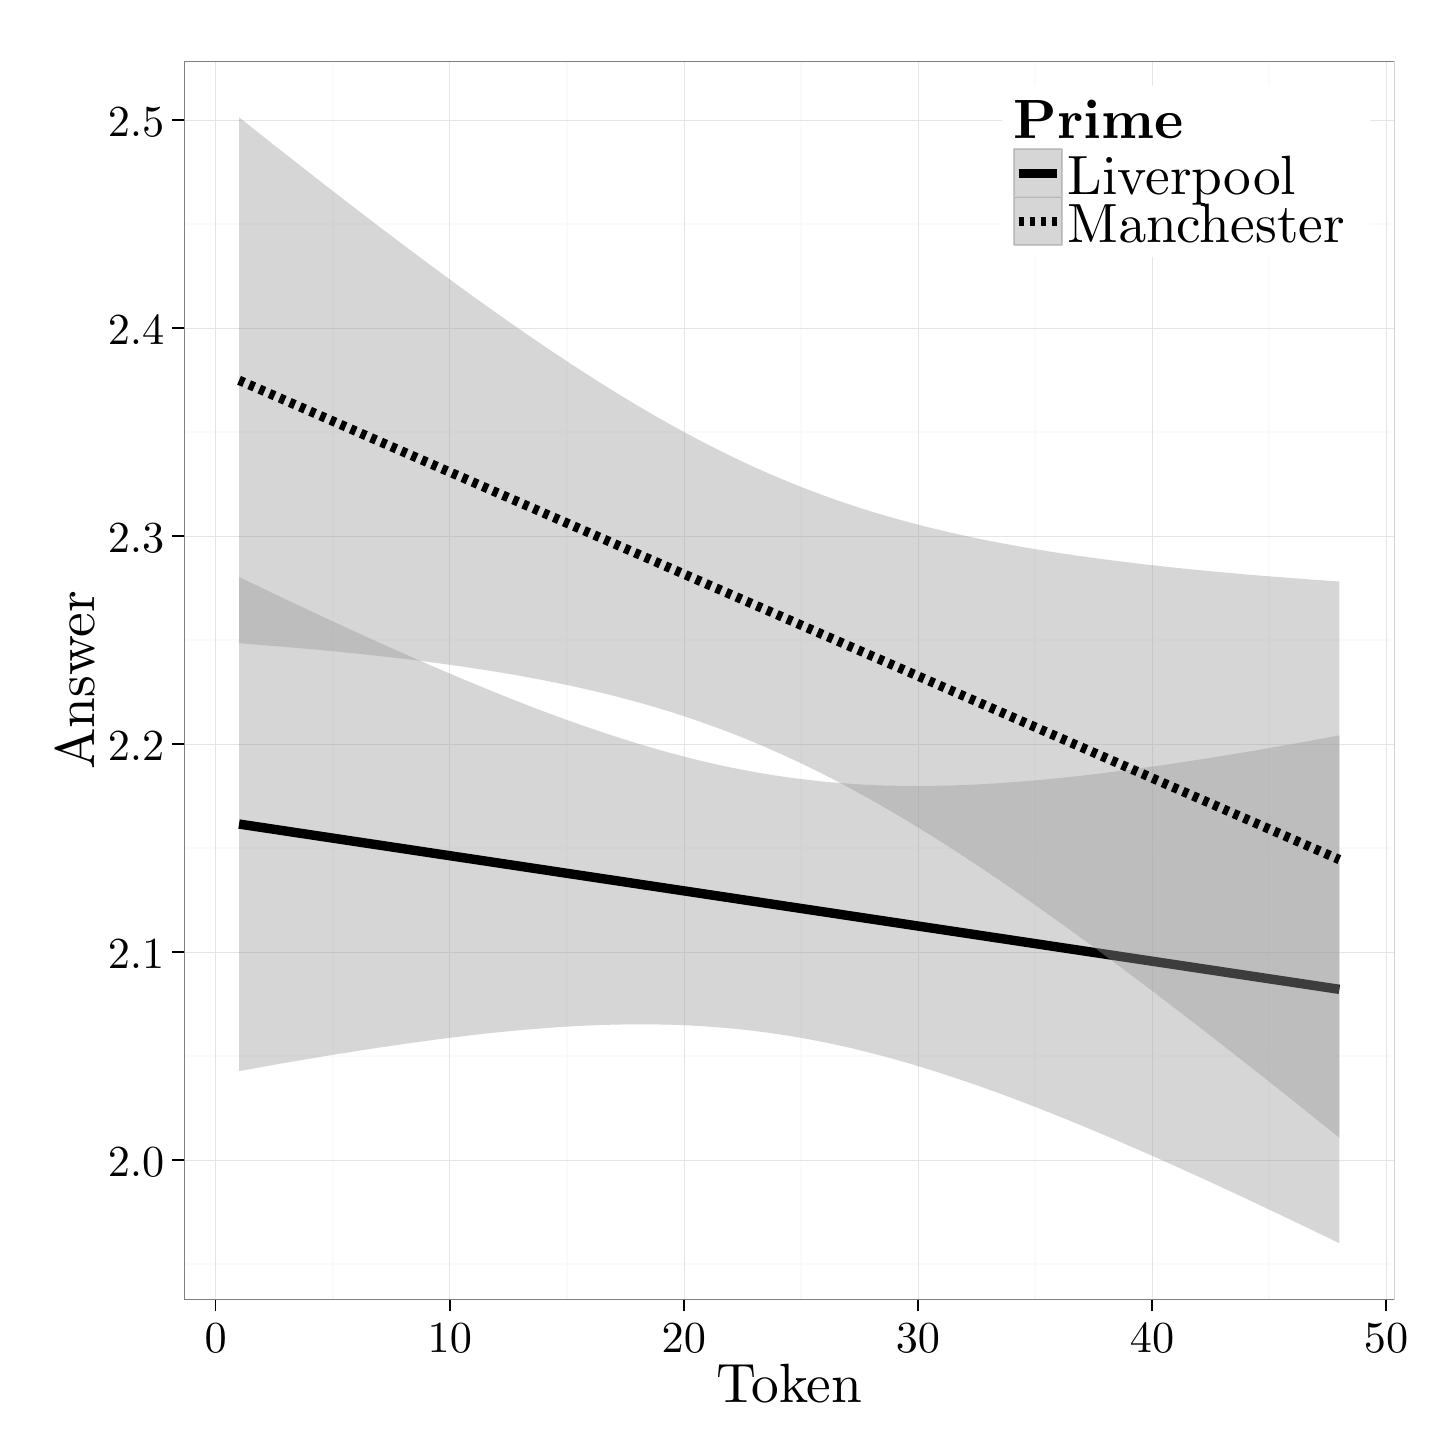
\begin{tikzpicture}[x=1pt,y=1pt]
\definecolor{fillColor}{RGB}{255,255,255}
\path[use as bounding box,fill=fillColor,fill opacity=0.00] (0,0) rectangle (505.89,505.89);
\begin{scope}
\path[clip] (  0.00,  0.00) rectangle (505.89,505.89);
\definecolor{drawColor}{RGB}{255,255,255}
\definecolor{fillColor}{RGB}{255,255,255}

\path[draw=drawColor,line width= 0.6pt,line join=round,line cap=round,fill=fillColor] (  0.00, -0.00) rectangle (505.89,505.89);
\end{scope}
\begin{scope}
\path[clip] ( 56.50, 46.31) rectangle (493.85,493.84);
\definecolor{fillColor}{RGB}{255,255,255}

\path[fill=fillColor] ( 56.50, 46.31) rectangle (493.85,493.84);
\definecolor{drawColor}{gray}{0.98}

\path[draw=drawColor,line width= 0.6pt,line join=round] ( 56.50, 59.23) --
	(493.85, 59.23);

\path[draw=drawColor,line width= 0.6pt,line join=round] ( 56.50,134.37) --
	(493.85,134.37);

\path[draw=drawColor,line width= 0.6pt,line join=round] ( 56.50,209.51) --
	(493.85,209.51);

\path[draw=drawColor,line width= 0.6pt,line join=round] ( 56.50,284.65) --
	(493.85,284.65);

\path[draw=drawColor,line width= 0.6pt,line join=round] ( 56.50,359.79) --
	(493.85,359.79);

\path[draw=drawColor,line width= 0.6pt,line join=round] ( 56.50,434.93) --
	(493.85,434.93);

\path[draw=drawColor,line width= 0.6pt,line join=round] (110.22, 46.31) --
	(110.22,493.84);

\path[draw=drawColor,line width= 0.6pt,line join=round] (194.81, 46.31) --
	(194.81,493.84);

\path[draw=drawColor,line width= 0.6pt,line join=round] (279.40, 46.31) --
	(279.40,493.84);

\path[draw=drawColor,line width= 0.6pt,line join=round] (364.00, 46.31) --
	(364.00,493.84);

\path[draw=drawColor,line width= 0.6pt,line join=round] (448.59, 46.31) --
	(448.59,493.84);
\definecolor{drawColor}{gray}{0.90}

\path[draw=drawColor,line width= 0.2pt,line join=round] ( 56.50, 96.80) --
	(493.85, 96.80);

\path[draw=drawColor,line width= 0.2pt,line join=round] ( 56.50,171.94) --
	(493.85,171.94);

\path[draw=drawColor,line width= 0.2pt,line join=round] ( 56.50,247.08) --
	(493.85,247.08);

\path[draw=drawColor,line width= 0.2pt,line join=round] ( 56.50,322.22) --
	(493.85,322.22);

\path[draw=drawColor,line width= 0.2pt,line join=round] ( 56.50,397.36) --
	(493.85,397.36);

\path[draw=drawColor,line width= 0.2pt,line join=round] ( 56.50,472.49) --
	(493.85,472.49);

\path[draw=drawColor,line width= 0.2pt,line join=round] ( 67.92, 46.31) --
	( 67.92,493.84);

\path[draw=drawColor,line width= 0.2pt,line join=round] (152.52, 46.31) --
	(152.52,493.84);

\path[draw=drawColor,line width= 0.2pt,line join=round] (237.11, 46.31) --
	(237.11,493.84);

\path[draw=drawColor,line width= 0.2pt,line join=round] (321.70, 46.31) --
	(321.70,493.84);

\path[draw=drawColor,line width= 0.2pt,line join=round] (406.29, 46.31) --
	(406.29,493.84);

\path[draw=drawColor,line width= 0.2pt,line join=round] (490.88, 46.31) --
	(490.88,493.84);
\definecolor{fillColor}{RGB}{153,153,153}

\path[fill=fillColor,fill opacity=0.40] ( 76.38,307.40) --
	( 81.42,304.97) --
	( 86.45,302.56) --
	( 91.48,300.16) --
	( 96.51,297.78) --
	(101.55,295.41) --
	(106.58,293.06) --
	(111.61,290.72) --
	(116.64,288.40) --
	(121.68,286.10) --
	(126.71,283.82) --
	(131.74,281.56) --
	(136.78,279.32) --
	(141.81,277.11) --
	(146.84,274.92) --
	(151.87,272.76) --
	(156.91,270.63) --
	(161.94,268.54) --
	(166.97,266.47) --
	(172.00,264.44) --
	(177.04,262.45) --
	(182.07,260.49) --
	(187.10,258.58) --
	(192.13,256.72) --
	(197.17,254.90) --
	(202.20,253.13) --
	(207.23,251.42) --
	(212.27,249.76) --
	(217.30,248.17) --
	(222.33,246.63) --
	(227.36,245.16) --
	(232.40,243.76) --
	(237.43,242.43) --
	(242.46,241.17) --
	(247.49,239.99) --
	(252.53,238.89) --
	(257.56,237.87) --
	(262.59,236.92) --
	(267.63,236.06) --
	(272.66,235.28) --
	(277.69,234.59) --
	(282.72,233.98) --
	(287.76,233.44) --
	(292.79,232.99) --
	(297.82,232.62) --
	(302.85,232.32) --
	(307.89,232.10) --
	(312.92,231.95) --
	(317.95,231.88) --
	(322.98,231.86) --
	(328.02,231.92) --
	(333.05,232.03) --
	(338.08,232.20) --
	(343.12,232.43) --
	(348.15,232.71) --
	(353.18,233.03) --
	(358.21,233.41) --
	(363.25,233.83) --
	(368.28,234.29) --
	(373.31,234.79) --
	(378.34,235.32) --
	(383.38,235.89) --
	(388.41,236.49) --
	(393.44,237.12) --
	(398.48,237.78) --
	(403.51,238.47) --
	(408.54,239.18) --
	(413.57,239.92) --
	(418.61,240.67) --
	(423.64,241.45) --
	(428.67,242.25) --
	(433.70,243.06) --
	(438.74,243.90) --
	(443.77,244.75) --
	(448.80,245.61) --
	(453.84,246.49) --
	(458.87,247.38) --
	(463.90,248.29) --
	(468.93,249.21) --
	(473.97,250.14) --
	(473.97, 66.65) --
	(468.93, 69.09) --
	(463.90, 71.52) --
	(458.87, 73.94) --
	(453.84, 76.34) --
	(448.80, 78.73) --
	(443.77, 81.11) --
	(438.74, 83.47) --
	(433.70, 85.82) --
	(428.67, 88.15) --
	(423.64, 90.46) --
	(418.61, 92.74) --
	(413.57, 95.01) --
	(408.54, 97.26) --
	(403.51, 99.49) --
	(398.48,101.68) --
	(393.44,103.86) --
	(388.41,106.00) --
	(383.38,108.11) --
	(378.34,110.19) --
	(373.31,112.24) --
	(368.28,114.25) --
	(363.25,116.22) --
	(358.21,118.15) --
	(353.18,120.04) --
	(348.15,121.88) --
	(343.12,123.67) --
	(338.08,125.41) --
	(333.05,127.09) --
	(328.02,128.72) --
	(322.98,130.28) --
	(317.95,131.78) --
	(312.92,133.22) --
	(307.89,134.58) --
	(302.85,135.87) --
	(297.82,137.09) --
	(292.79,138.23) --
	(287.76,139.29) --
	(282.72,140.27) --
	(277.69,141.17) --
	(272.66,141.98) --
	(267.63,142.72) --
	(262.59,143.37) --
	(257.56,143.94) --
	(252.53,144.43) --
	(247.49,144.83) --
	(242.46,145.17) --
	(237.43,145.42) --
	(232.40,145.60) --
	(227.36,145.71) --
	(222.33,145.76) --
	(217.30,145.73) --
	(212.27,145.65) --
	(207.23,145.50) --
	(202.20,145.30) --
	(197.17,145.05) --
	(192.13,144.74) --
	(187.10,144.39) --
	(182.07,143.99) --
	(177.04,143.55) --
	(172.00,143.07) --
	(166.97,142.55) --
	(161.94,142.00) --
	(156.91,141.41) --
	(151.87,140.79) --
	(146.84,140.14) --
	(141.81,139.47) --
	(136.78,138.77) --
	(131.74,138.04) --
	(126.71,137.30) --
	(121.68,136.53) --
	(116.64,135.74) --
	(111.61,134.93) --
	(106.58,134.11) --
	(101.55,133.27) --
	( 96.51,132.41) --
	( 91.48,131.54) --
	( 86.45,130.65) --
	( 81.42,129.75) --
	( 76.38,128.84) --
	cycle;
\definecolor{drawColor}{RGB}{0,0,0}

\path[draw=drawColor,line width= 3.4pt,line join=round] ( 76.38,218.12) --
	( 81.42,217.36) --
	( 86.45,216.61) --
	( 91.48,215.85) --
	( 96.51,215.09) --
	(101.55,214.34) --
	(106.58,213.58) --
	(111.61,212.83) --
	(116.64,212.07) --
	(121.68,211.31) --
	(126.71,210.56) --
	(131.74,209.80) --
	(136.78,209.05) --
	(141.81,208.29) --
	(146.84,207.53) --
	(151.87,206.78) --
	(156.91,206.02) --
	(161.94,205.27) --
	(166.97,204.51) --
	(172.00,203.75) --
	(177.04,203.00) --
	(182.07,202.24) --
	(187.10,201.49) --
	(192.13,200.73) --
	(197.17,199.97) --
	(202.20,199.22) --
	(207.23,198.46) --
	(212.27,197.71) --
	(217.30,196.95) --
	(222.33,196.19) --
	(227.36,195.44) --
	(232.40,194.68) --
	(237.43,193.93) --
	(242.46,193.17) --
	(247.49,192.41) --
	(252.53,191.66) --
	(257.56,190.90) --
	(262.59,190.15) --
	(267.63,189.39) --
	(272.66,188.63) --
	(277.69,187.88) --
	(282.72,187.12) --
	(287.76,186.37) --
	(292.79,185.61) --
	(297.82,184.85) --
	(302.85,184.10) --
	(307.89,183.34) --
	(312.92,182.59) --
	(317.95,181.83) --
	(322.98,181.07) --
	(328.02,180.32) --
	(333.05,179.56) --
	(338.08,178.81) --
	(343.12,178.05) --
	(348.15,177.29) --
	(353.18,176.54) --
	(358.21,175.78) --
	(363.25,175.03) --
	(368.28,174.27) --
	(373.31,173.51) --
	(378.34,172.76) --
	(383.38,172.00) --
	(388.41,171.25) --
	(393.44,170.49) --
	(398.48,169.73) --
	(403.51,168.98) --
	(408.54,168.22) --
	(413.57,167.47) --
	(418.61,166.71) --
	(423.64,165.95) --
	(428.67,165.20) --
	(433.70,164.44) --
	(438.74,163.69) --
	(443.77,162.93) --
	(448.80,162.17) --
	(453.84,161.42) --
	(458.87,160.66) --
	(463.90,159.91) --
	(468.93,159.15) --
	(473.97,158.39);

\path[fill=fillColor,fill opacity=0.40] ( 76.38,473.50) --
	( 81.42,469.50) --
	( 86.45,465.51) --
	( 91.48,461.54) --
	( 96.51,457.58) --
	(101.55,453.64) --
	(106.58,449.71) --
	(111.61,445.81) --
	(116.64,441.92) --
	(121.68,438.06) --
	(126.71,434.22) --
	(131.74,430.40) --
	(136.78,426.61) --
	(141.81,422.84) --
	(146.84,419.10) --
	(151.87,415.40) --
	(156.91,411.73) --
	(161.94,408.09) --
	(166.97,404.49) --
	(172.00,400.93) --
	(177.04,397.41) --
	(182.07,393.94) --
	(187.10,390.51) --
	(192.13,387.14) --
	(197.17,383.82) --
	(202.20,380.56) --
	(207.23,377.36) --
	(212.27,374.23) --
	(217.30,371.16) --
	(222.33,368.16) --
	(227.36,365.24) --
	(232.40,362.39) --
	(237.43,359.63) --
	(242.46,356.94) --
	(247.49,354.35) --
	(252.53,351.84) --
	(257.56,349.41) --
	(262.59,347.08) --
	(267.63,344.84) --
	(272.66,342.70) --
	(277.69,340.64) --
	(282.72,338.67) --
	(287.76,336.80) --
	(292.79,335.01) --
	(297.82,333.30) --
	(302.85,331.68) --
	(307.89,330.14) --
	(312.92,328.68) --
	(317.95,327.29) --
	(322.98,325.97) --
	(328.02,324.72) --
	(333.05,323.53) --
	(338.08,322.40) --
	(343.12,321.34) --
	(348.15,320.32) --
	(353.18,319.36) --
	(358.21,318.45) --
	(363.25,317.58) --
	(368.28,316.75) --
	(373.31,315.97) --
	(378.34,315.22) --
	(383.38,314.51) --
	(388.41,313.83) --
	(393.44,313.18) --
	(398.48,312.56) --
	(403.51,311.96) --
	(408.54,311.40) --
	(413.57,310.85) --
	(418.61,310.33) --
	(423.64,309.83) --
	(428.67,309.35) --
	(433.70,308.89) --
	(438.74,308.45) --
	(443.77,308.02) --
	(448.80,307.61) --
	(453.84,307.22) --
	(458.87,306.83) --
	(463.90,306.46) --
	(468.93,306.11) --
	(473.97,305.76) --
	(473.97,104.79) --
	(468.93,108.83) --
	(463.90,112.86) --
	(458.87,116.87) --
	(453.84,120.87) --
	(448.80,124.86) --
	(443.77,128.84) --
	(438.74,132.79) --
	(433.70,136.73) --
	(428.67,140.66) --
	(423.64,144.56) --
	(418.61,148.45) --
	(413.57,152.31) --
	(408.54,156.15) --
	(403.51,159.97) --
	(398.48,163.76) --
	(393.44,167.53) --
	(388.41,171.26) --
	(383.38,174.97) --
	(378.34,178.64) --
	(373.31,182.27) --
	(368.28,185.87) --
	(363.25,189.43) --
	(358.21,192.95) --
	(353.18,196.42) --
	(348.15,199.84) --
	(343.12,203.21) --
	(338.08,206.53) --
	(333.05,209.79) --
	(328.02,212.99) --
	(322.98,216.12) --
	(317.95,219.19) --
	(312.92,222.18) --
	(307.89,225.10) --
	(302.85,227.94) --
	(297.82,230.71) --
	(292.79,233.39) --
	(287.76,235.98) --
	(282.72,238.49) --
	(277.69,240.91) --
	(272.66,243.24) --
	(267.63,245.47) --
	(262.59,247.62) --
	(257.56,249.67) --
	(252.53,251.63) --
	(247.49,253.51) --
	(242.46,255.30) --
	(237.43,257.00) --
	(232.40,258.62) --
	(227.36,260.16) --
	(222.33,261.62) --
	(217.30,263.00) --
	(212.27,264.32) --
	(207.23,265.57) --
	(202.20,266.75) --
	(197.17,267.88) --
	(192.13,268.94) --
	(187.10,269.95) --
	(182.07,270.91) --
	(177.04,271.83) --
	(172.00,272.69) --
	(166.97,273.52) --
	(161.94,274.30) --
	(156.91,275.05) --
	(151.87,275.76) --
	(146.84,276.44) --
	(141.81,277.09) --
	(136.78,277.71) --
	(131.74,278.30) --
	(126.71,278.87) --
	(121.68,279.41) --
	(116.64,279.93) --
	(111.61,280.43) --
	(106.58,280.91) --
	(101.55,281.37) --
	( 96.51,281.81) --
	( 91.48,282.24) --
	( 86.45,282.65) --
	( 81.42,283.04) --
	( 76.38,283.43) --
	cycle;

\path[draw=drawColor,line width= 3.4pt,dash pattern=on 2pt off 2pt ,line join=round] ( 76.38,378.46) --
	( 81.42,376.27) --
	( 86.45,374.08) --
	( 91.48,371.89) --
	( 96.51,369.69) --
	(101.55,367.50) --
	(106.58,365.31) --
	(111.61,363.12) --
	(116.64,360.93) --
	(121.68,358.73) --
	(126.71,356.54) --
	(131.74,354.35) --
	(136.78,352.16) --
	(141.81,349.96) --
	(146.84,347.77) --
	(151.87,345.58) --
	(156.91,343.39) --
	(161.94,341.20) --
	(166.97,339.00) --
	(172.00,336.81) --
	(177.04,334.62) --
	(182.07,332.43) --
	(187.10,330.23) --
	(192.13,328.04) --
	(197.17,325.85) --
	(202.20,323.66) --
	(207.23,321.47) --
	(212.27,319.27) --
	(217.30,317.08) --
	(222.33,314.89) --
	(227.36,312.70) --
	(232.40,310.50) --
	(237.43,308.31) --
	(242.46,306.12) --
	(247.49,303.93) --
	(252.53,301.73) --
	(257.56,299.54) --
	(262.59,297.35) --
	(267.63,295.16) --
	(272.66,292.97) --
	(277.69,290.77) --
	(282.72,288.58) --
	(287.76,286.39) --
	(292.79,284.20) --
	(297.82,282.00) --
	(302.85,279.81) --
	(307.89,277.62) --
	(312.92,275.43) --
	(317.95,273.24) --
	(322.98,271.04) --
	(328.02,268.85) --
	(333.05,266.66) --
	(338.08,264.47) --
	(343.12,262.27) --
	(348.15,260.08) --
	(353.18,257.89) --
	(358.21,255.70) --
	(363.25,253.51) --
	(368.28,251.31) --
	(373.31,249.12) --
	(378.34,246.93) --
	(383.38,244.74) --
	(388.41,242.54) --
	(393.44,240.35) --
	(398.48,238.16) --
	(403.51,235.97) --
	(408.54,233.77) --
	(413.57,231.58) --
	(418.61,229.39) --
	(423.64,227.20) --
	(428.67,225.01) --
	(433.70,222.81) --
	(438.74,220.62) --
	(443.77,218.43) --
	(448.80,216.24) --
	(453.84,214.04) --
	(458.87,211.85) --
	(463.90,209.66) --
	(468.93,207.47) --
	(473.97,205.28);
\definecolor{drawColor}{gray}{0.50}

\path[draw=drawColor,line width= 0.6pt,line join=round,line cap=round] ( 56.50, 46.31) rectangle (493.85,493.84);
\end{scope}
\begin{scope}
\path[clip] (  0.00,  0.00) rectangle (505.89,505.89);
\definecolor{drawColor}{RGB}{0,0,0}

\node[text=drawColor,anchor=base east,inner sep=0pt, outer sep=0pt, scale=  1.60] at ( 49.39, 90.77) {2.0};

\node[text=drawColor,anchor=base east,inner sep=0pt, outer sep=0pt, scale=  1.60] at ( 49.39,165.91) {2.1};

\node[text=drawColor,anchor=base east,inner sep=0pt, outer sep=0pt, scale=  1.60] at ( 49.39,241.05) {2.2};

\node[text=drawColor,anchor=base east,inner sep=0pt, outer sep=0pt, scale=  1.60] at ( 49.39,316.18) {2.3};

\node[text=drawColor,anchor=base east,inner sep=0pt, outer sep=0pt, scale=  1.60] at ( 49.39,391.32) {2.4};

\node[text=drawColor,anchor=base east,inner sep=0pt, outer sep=0pt, scale=  1.60] at ( 49.39,466.46) {2.5};
\end{scope}
\begin{scope}
\path[clip] (  0.00,  0.00) rectangle (505.89,505.89);
\definecolor{drawColor}{RGB}{0,0,0}

\path[draw=drawColor,line width= 0.6pt,line join=round] ( 52.24, 96.80) --
	( 56.50, 96.80);

\path[draw=drawColor,line width= 0.6pt,line join=round] ( 52.24,171.94) --
	( 56.50,171.94);

\path[draw=drawColor,line width= 0.6pt,line join=round] ( 52.24,247.08) --
	( 56.50,247.08);

\path[draw=drawColor,line width= 0.6pt,line join=round] ( 52.24,322.22) --
	( 56.50,322.22);

\path[draw=drawColor,line width= 0.6pt,line join=round] ( 52.24,397.36) --
	( 56.50,397.36);

\path[draw=drawColor,line width= 0.6pt,line join=round] ( 52.24,472.49) --
	( 56.50,472.49);
\end{scope}
\begin{scope}
\path[clip] (  0.00,  0.00) rectangle (505.89,505.89);
\definecolor{drawColor}{RGB}{0,0,0}

\path[draw=drawColor,line width= 0.6pt,line join=round] ( 67.92, 42.04) --
	( 67.92, 46.31);

\path[draw=drawColor,line width= 0.6pt,line join=round] (152.52, 42.04) --
	(152.52, 46.31);

\path[draw=drawColor,line width= 0.6pt,line join=round] (237.11, 42.04) --
	(237.11, 46.31);

\path[draw=drawColor,line width= 0.6pt,line join=round] (321.70, 42.04) --
	(321.70, 46.31);

\path[draw=drawColor,line width= 0.6pt,line join=round] (406.29, 42.04) --
	(406.29, 46.31);

\path[draw=drawColor,line width= 0.6pt,line join=round] (490.88, 42.04) --
	(490.88, 46.31);
\end{scope}
\begin{scope}
\path[clip] (  0.00,  0.00) rectangle (505.89,505.89);
\definecolor{drawColor}{RGB}{0,0,0}

\node[text=drawColor,anchor=base,inner sep=0pt, outer sep=0pt, scale=  1.60] at ( 67.92, 27.13) {0};

\node[text=drawColor,anchor=base,inner sep=0pt, outer sep=0pt, scale=  1.60] at (152.52, 27.13) {10};

\node[text=drawColor,anchor=base,inner sep=0pt, outer sep=0pt, scale=  1.60] at (237.11, 27.13) {20};

\node[text=drawColor,anchor=base,inner sep=0pt, outer sep=0pt, scale=  1.60] at (321.70, 27.13) {30};

\node[text=drawColor,anchor=base,inner sep=0pt, outer sep=0pt, scale=  1.60] at (406.29, 27.13) {40};

\node[text=drawColor,anchor=base,inner sep=0pt, outer sep=0pt, scale=  1.60] at (490.88, 27.13) {50};
\end{scope}
\begin{scope}
\path[clip] (  0.00,  0.00) rectangle (505.89,505.89);
\definecolor{drawColor}{RGB}{0,0,0}

\node[text=drawColor,anchor=base,inner sep=0pt, outer sep=0pt, scale=  2.00] at (275.17,  9.03) {Token};
\end{scope}
\begin{scope}
\path[clip] (  0.00,  0.00) rectangle (505.89,505.89);
\definecolor{drawColor}{RGB}{0,0,0}

\node[text=drawColor,rotate= 90.00,anchor=base,inner sep=0pt, outer sep=0pt, scale=  2.00] at ( 24.12,270.08) {Answer};
\end{scope}
\begin{scope}
\path[clip] (  0.00,  0.00) rectangle (505.89,505.89);
\definecolor{fillColor}{RGB}{255,255,255}

\path[fill=fillColor] (352.06,423.00) rectangle (484.98,484.98);
\end{scope}
\begin{scope}
\path[clip] (  0.00,  0.00) rectangle (505.89,505.89);
\definecolor{drawColor}{RGB}{0,0,0}

\node[text=drawColor,anchor=base west,inner sep=0pt, outer sep=0pt, scale=  2.00] at (356.32,465.96) {\bfseries Prime};
\end{scope}
\begin{scope}
\path[clip] (  0.00,  0.00) rectangle (505.89,505.89);
\definecolor{drawColor}{gray}{0.80}
\definecolor{fillColor}{RGB}{255,255,255}

\path[draw=drawColor,line width= 0.6pt,line join=round,line cap=round,fill=fillColor] (356.32,444.61) rectangle (373.67,461.96);
\end{scope}
\begin{scope}
\path[clip] (  0.00,  0.00) rectangle (505.89,505.89);
\definecolor{fillColor}{RGB}{153,153,153}

\path[fill=fillColor,fill opacity=0.40] (356.32,444.61) rectangle (373.67,461.96);
\definecolor{drawColor}{RGB}{0,0,0}

\path[draw=drawColor,line width= 3.4pt,line join=round] (358.06,453.29) -- (371.93,453.29);
\end{scope}
\begin{scope}
\path[clip] (  0.00,  0.00) rectangle (505.89,505.89);
\definecolor{drawColor}{gray}{0.80}
\definecolor{fillColor}{RGB}{255,255,255}

\path[draw=drawColor,line width= 0.6pt,line join=round,line cap=round,fill=fillColor] (356.32,427.27) rectangle (373.67,444.61);
\end{scope}
\begin{scope}
\path[clip] (  0.00,  0.00) rectangle (505.89,505.89);
\definecolor{fillColor}{RGB}{153,153,153}

\path[fill=fillColor,fill opacity=0.40] (356.32,427.27) rectangle (373.67,444.61);
\definecolor{drawColor}{RGB}{0,0,0}

\path[draw=drawColor,line width= 3.4pt,dash pattern=on 2pt off 2pt ,line join=round] (358.06,435.94) -- (371.93,435.94);
\end{scope}
\begin{scope}
\path[clip] (  0.00,  0.00) rectangle (505.89,505.89);
\definecolor{drawColor}{RGB}{0,0,0}

\node[text=drawColor,anchor=base west,inner sep=0pt, outer sep=0pt, scale=  2.00] at (375.84,445.75) {Liverpool};
\end{scope}
\begin{scope}
\path[clip] (  0.00,  0.00) rectangle (505.89,505.89);
\definecolor{drawColor}{RGB}{0,0,0}

\node[text=drawColor,anchor=base west,inner sep=0pt, outer sep=0pt, scale=  2.00] at (375.84,428.40) {Manchester};
\end{scope}
\end{tikzpicture}
} 
	\caption{\textsc{nurse} (perception) by token}
	\label{fig.scatter.nurse.ext.token}
\end{figure}

The influence of token (i.e. the point in time the item was presented in the course of the experiment) on which answer was chosen is slightly more straightforward than the one of age for happ\textsc{y} stimuli.
The coefficient from the mixed-effects model (\ensuremath{-0.011}) implies a weak downward slope and this is visible in Figure \ref{fig.scatter.nurse.ext.token}.
Just as with age for happ\textsc{y} there is a substantial amount of variation.
Nevertheless, it seems clear that subjects are increasingly less likely to perceive the higher-numbered tokens and tend more and more towards the lower (hyper-)\isi{Mancunian} end of the answer range the further they progress in the experiment.
The dashed regression line for the `\isi{Manchester}' \isi{priming} condition is above the one for the `\isi{Liverpool}' group (reflecting the fact that subjects primed for `\isi{Manchester}' were more likely to respond with Liverpool-like tokens), but the distance between conditions tends to get smaller in the course of the test because the slope is steeper for the `\isi{Manchester}' condition. That is to say participants primed for \isi{Manchester} change their behaviour more drastically than the other group.
In the last third of the experiment, the two conditions seem much more aligned: the lines are closer to each other than in the beginning and the standard error ranges start overlapping considerably.
For the last ten items or so the regression lines are within the error range of the other group, indicating that the answers given in the two groups are not significantly different (anymore).

\begin{figure}[h]
	\centering
		\definecolor{shadecolor}{rgb}{0.969, 0.969, 0.969}
		\resizebox{.49\linewidth}{!}{% Created by tikzDevice version 0.8.1 on 2016-02-09 02:18:55
% !TEX encoding = UTF-8 Unicode
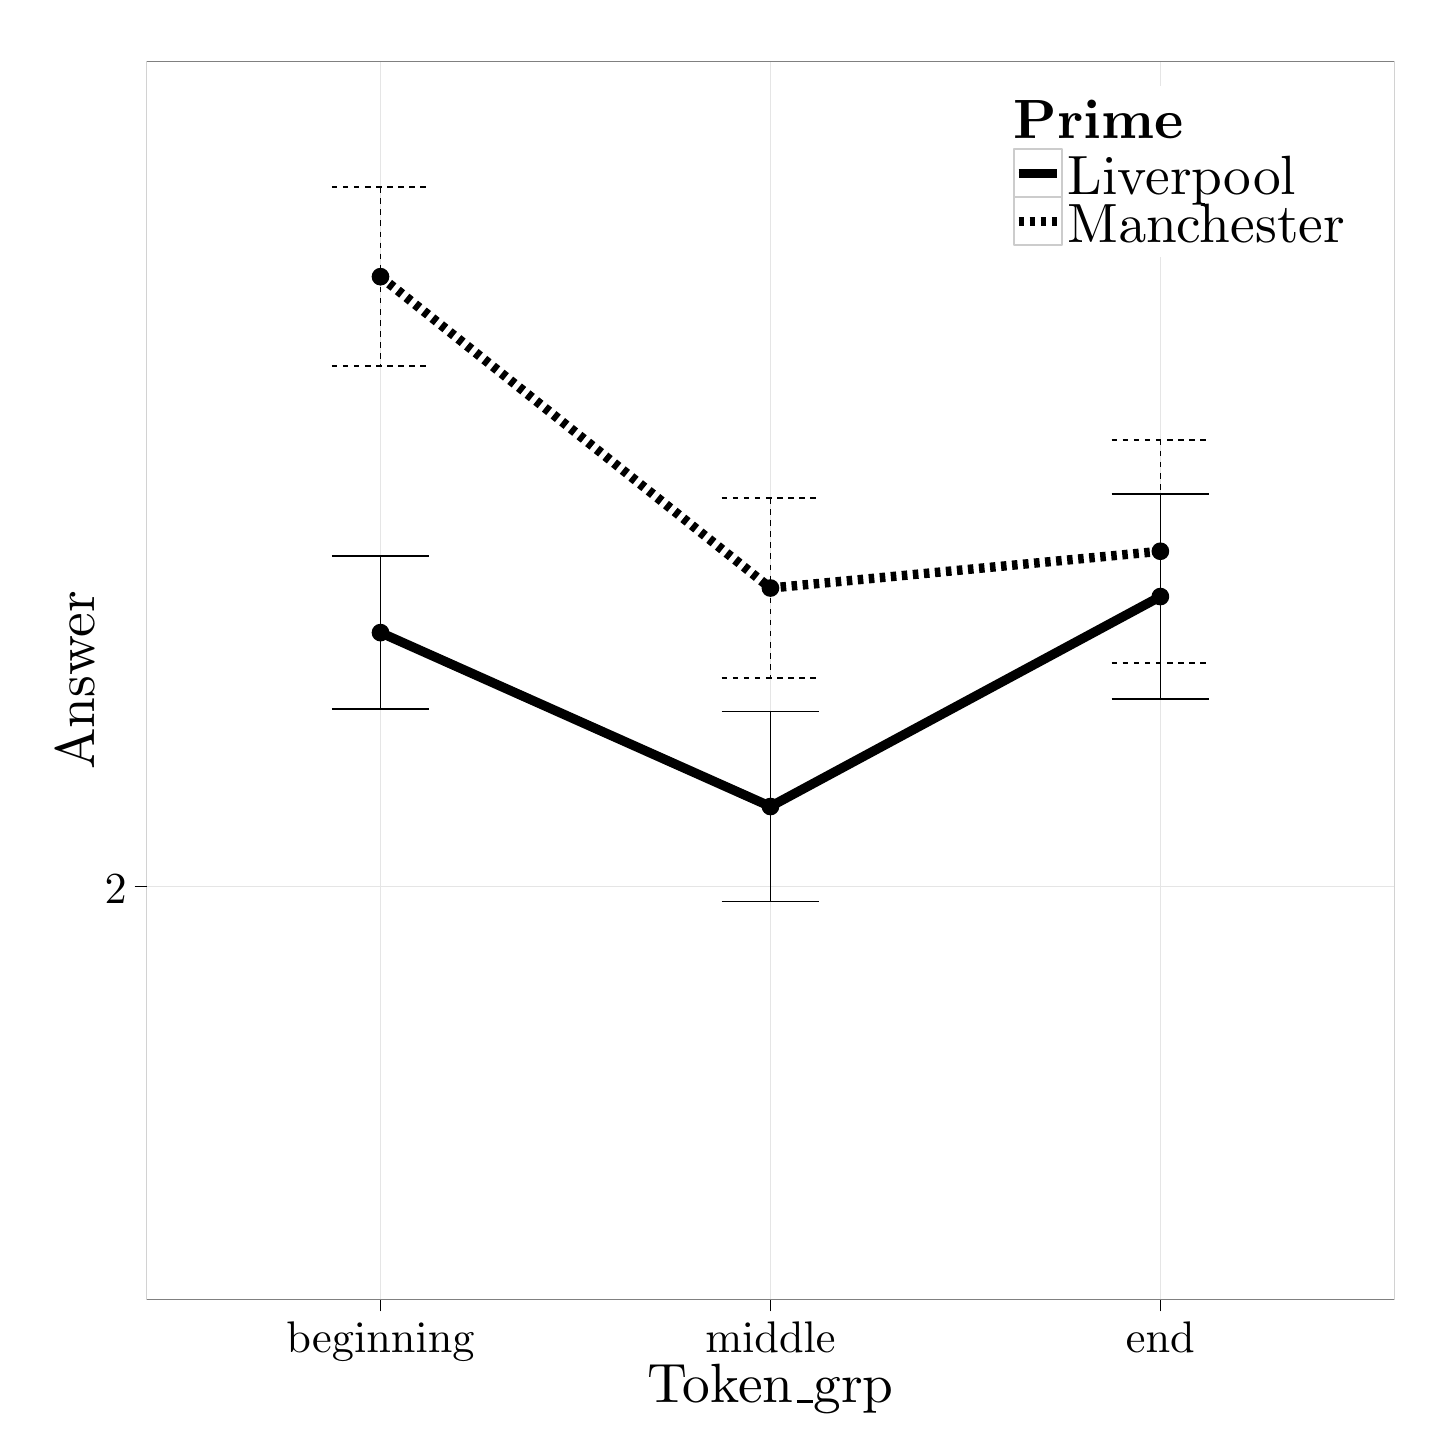
\begin{tikzpicture}[x=1pt,y=1pt]
\definecolor{fillColor}{RGB}{255,255,255}
\path[use as bounding box,fill=fillColor,fill opacity=0.00] (0,0) rectangle (505.89,505.89);
\begin{scope}
\path[clip] (  0.00,  0.00) rectangle (505.89,505.89);
\definecolor{drawColor}{RGB}{255,255,255}
\definecolor{fillColor}{RGB}{255,255,255}

\path[draw=drawColor,line width= 0.6pt,line join=round,line cap=round,fill=fillColor] (  0.00, -0.00) rectangle (505.89,505.89);
\end{scope}
\begin{scope}
\path[clip] ( 42.95, 46.31) rectangle (493.85,493.84);
\definecolor{fillColor}{RGB}{255,255,255}

\path[fill=fillColor] ( 42.95, 46.31) rectangle (493.85,493.84);
\definecolor{drawColor}{gray}{0.90}

\path[draw=drawColor,line width= 0.2pt,line join=round] ( 42.95,195.49) --
	(493.85,195.49);

\path[draw=drawColor,line width= 0.2pt,line join=round] (127.49, 46.31) --
	(127.49,493.84);

\path[draw=drawColor,line width= 0.2pt,line join=round] (268.40, 46.31) --
	(268.40,493.84);

\path[draw=drawColor,line width= 0.2pt,line join=round] (409.30, 46.31) --
	(409.30,493.84);
\definecolor{fillColor}{RGB}{0,0,0}

\path[fill=fillColor] (127.49,287.29) circle (  3.20);

\path[fill=fillColor] (127.49,415.90) circle (  3.20);

\path[fill=fillColor] (268.40,224.45) circle (  3.20);

\path[fill=fillColor] (268.40,303.40) circle (  3.20);

\path[fill=fillColor] (409.30,300.32) circle (  3.20);

\path[fill=fillColor] (409.30,316.69) circle (  3.20);
\definecolor{drawColor}{RGB}{0,0,0}

\path[draw=drawColor,line width= 3.4pt,line join=round] (127.49,287.29) --
	(268.40,224.45) --
	(409.30,300.32);

\path[draw=drawColor,line width= 3.4pt,dash pattern=on 2pt off 2pt ,line join=round] (127.49,415.90) --
	(268.40,303.40) --
	(409.30,316.69);

\path[draw=drawColor,line width= 0.6pt,line join=round] (109.88,314.98) --
	(145.11,314.98);

\path[draw=drawColor,line width= 0.6pt,line join=round] (127.49,314.98) --
	(127.49,259.60);

\path[draw=drawColor,line width= 0.6pt,line join=round] (109.88,259.60) --
	(145.11,259.60);

\path[draw=drawColor,line width= 0.6pt,line join=round] (250.79,258.78) --
	(286.01,258.78);

\path[draw=drawColor,line width= 0.6pt,line join=round] (268.40,258.78) --
	(268.40,190.13);

\path[draw=drawColor,line width= 0.6pt,line join=round] (250.79,190.13) --
	(286.01,190.13);

\path[draw=drawColor,line width= 0.6pt,line join=round] (391.69,337.27) --
	(426.92,337.27);

\path[draw=drawColor,line width= 0.6pt,line join=round] (409.30,337.27) --
	(409.30,263.36);

\path[draw=drawColor,line width= 0.6pt,line join=round] (391.69,263.36) --
	(426.92,263.36);

\path[draw=drawColor,line width= 0.6pt,dash pattern=on 2pt off 2pt ,line join=round] (109.88,448.23) --
	(145.11,448.23);

\path[draw=drawColor,line width= 0.6pt,dash pattern=on 2pt off 2pt ,line join=round] (127.49,448.23) --
	(127.49,383.56);

\path[draw=drawColor,line width= 0.6pt,dash pattern=on 2pt off 2pt ,line join=round] (109.88,383.56) --
	(145.11,383.56);

\path[draw=drawColor,line width= 0.6pt,dash pattern=on 2pt off 2pt ,line join=round] (250.79,335.90) --
	(286.01,335.90);

\path[draw=drawColor,line width= 0.6pt,dash pattern=on 2pt off 2pt ,line join=round] (268.40,335.90) --
	(268.40,270.91);

\path[draw=drawColor,line width= 0.6pt,dash pattern=on 2pt off 2pt ,line join=round] (250.79,270.91) --
	(286.01,270.91);

\path[draw=drawColor,line width= 0.6pt,dash pattern=on 2pt off 2pt ,line join=round] (391.69,356.96) --
	(426.92,356.96);

\path[draw=drawColor,line width= 0.6pt,dash pattern=on 2pt off 2pt ,line join=round] (409.30,356.96) --
	(409.30,276.43);

\path[draw=drawColor,line width= 0.6pt,dash pattern=on 2pt off 2pt ,line join=round] (391.69,276.43) --
	(426.92,276.43);
\definecolor{drawColor}{gray}{0.50}

\path[draw=drawColor,line width= 0.6pt,line join=round,line cap=round] ( 42.95, 46.31) rectangle (493.85,493.84);
\end{scope}
\begin{scope}
\path[clip] (  0.00,  0.00) rectangle (505.89,505.89);
\definecolor{drawColor}{RGB}{0,0,0}

\node[text=drawColor,anchor=base east,inner sep=0pt, outer sep=0pt, scale=  1.60] at ( 35.84,189.45) {2};
\end{scope}
\begin{scope}
\path[clip] (  0.00,  0.00) rectangle (505.89,505.89);
\definecolor{drawColor}{RGB}{0,0,0}

\path[draw=drawColor,line width= 0.6pt,line join=round] ( 38.68,195.49) --
	( 42.95,195.49);
\end{scope}
\begin{scope}
\path[clip] (  0.00,  0.00) rectangle (505.89,505.89);
\definecolor{drawColor}{RGB}{0,0,0}

\path[draw=drawColor,line width= 0.6pt,line join=round] (127.49, 42.04) --
	(127.49, 46.31);

\path[draw=drawColor,line width= 0.6pt,line join=round] (268.40, 42.04) --
	(268.40, 46.31);

\path[draw=drawColor,line width= 0.6pt,line join=round] (409.30, 42.04) --
	(409.30, 46.31);
\end{scope}
\begin{scope}
\path[clip] (  0.00,  0.00) rectangle (505.89,505.89);
\definecolor{drawColor}{RGB}{0,0,0}

\node[text=drawColor,anchor=base,inner sep=0pt, outer sep=0pt, scale=  1.60] at (127.49, 27.13) {beginning};

\node[text=drawColor,anchor=base,inner sep=0pt, outer sep=0pt, scale=  1.60] at (268.40, 27.13) {middle};

\node[text=drawColor,anchor=base,inner sep=0pt, outer sep=0pt, scale=  1.60] at (409.30, 27.13) {end};
\end{scope}
\begin{scope}
\path[clip] (  0.00,  0.00) rectangle (505.89,505.89);
\definecolor{drawColor}{RGB}{0,0,0}

\node[text=drawColor,anchor=base,inner sep=0pt, outer sep=0pt, scale=  2.00] at (268.40,  9.03) {Token{\_{}}grp};
\end{scope}
\begin{scope}
\path[clip] (  0.00,  0.00) rectangle (505.89,505.89);
\definecolor{drawColor}{RGB}{0,0,0}

\node[text=drawColor,rotate= 90.00,anchor=base,inner sep=0pt, outer sep=0pt, scale=  2.00] at ( 24.12,270.08) {Answer};
\end{scope}
\begin{scope}
\path[clip] (  0.00,  0.00) rectangle (505.89,505.89);
\definecolor{fillColor}{RGB}{255,255,255}

\path[fill=fillColor] (352.06,423.00) rectangle (484.98,484.98);
\end{scope}
\begin{scope}
\path[clip] (  0.00,  0.00) rectangle (505.89,505.89);
\definecolor{drawColor}{RGB}{0,0,0}

\node[text=drawColor,anchor=base west,inner sep=0pt, outer sep=0pt, scale=  2.00] at (356.32,465.96) {\bfseries Prime};
\end{scope}
\begin{scope}
\path[clip] (  0.00,  0.00) rectangle (505.89,505.89);
\definecolor{drawColor}{gray}{0.80}
\definecolor{fillColor}{RGB}{255,255,255}

\path[draw=drawColor,line width= 0.6pt,line join=round,line cap=round,fill=fillColor] (356.32,444.61) rectangle (373.67,461.96);
\end{scope}
\begin{scope}
\path[clip] (  0.00,  0.00) rectangle (505.89,505.89);
\definecolor{drawColor}{RGB}{0,0,0}

\path[draw=drawColor,line width= 3.4pt,line join=round] (358.06,453.29) -- (371.93,453.29);
\end{scope}
\begin{scope}
\path[clip] (  0.00,  0.00) rectangle (505.89,505.89);
\definecolor{drawColor}{RGB}{0,0,0}

\path[draw=drawColor,line width= 0.6pt,line join=round] (358.06,453.29) -- (371.93,453.29);
\end{scope}
\begin{scope}
\path[clip] (  0.00,  0.00) rectangle (505.89,505.89);
\definecolor{drawColor}{gray}{0.80}
\definecolor{fillColor}{RGB}{255,255,255}

\path[draw=drawColor,line width= 0.6pt,line join=round,line cap=round,fill=fillColor] (356.32,427.27) rectangle (373.67,444.61);
\end{scope}
\begin{scope}
\path[clip] (  0.00,  0.00) rectangle (505.89,505.89);
\definecolor{drawColor}{RGB}{0,0,0}

\path[draw=drawColor,line width= 3.4pt,dash pattern=on 2pt off 2pt ,line join=round] (358.06,435.94) -- (371.93,435.94);
\end{scope}
\begin{scope}
\path[clip] (  0.00,  0.00) rectangle (505.89,505.89);
\definecolor{drawColor}{RGB}{0,0,0}

\path[draw=drawColor,line width= 0.6pt,dash pattern=on 2pt off 2pt ,line join=round] (358.06,435.94) -- (371.93,435.94);
\end{scope}
\begin{scope}
\path[clip] (  0.00,  0.00) rectangle (505.89,505.89);
\definecolor{drawColor}{RGB}{0,0,0}

\node[text=drawColor,anchor=base west,inner sep=0pt, outer sep=0pt, scale=  2.00] at (375.84,445.75) {Liverpool};
\end{scope}
\begin{scope}
\path[clip] (  0.00,  0.00) rectangle (505.89,505.89);
\definecolor{drawColor}{RGB}{0,0,0}

\node[text=drawColor,anchor=base west,inner sep=0pt, outer sep=0pt, scale=  2.00] at (375.84,428.40) {Manchester};
\end{scope}
\end{tikzpicture}
} 
	\caption{\textsc{nurse} (perception) by token (grouped)}
	\label{fig.line.nurse.ext.token}
\end{figure}

Figure \ref{fig.line.nurse.ext.token} visualises the differences between \isi{priming} groups when responses are grouped with respect to whether they were given at the beginning (items 1--18), in the middle (items 19--36), or towards the end (items 37--48) of the experiment.
The dots mark the answer means in the respective phases of the test, \isi{priming} conditions are coded by line type as usual (dashed for `\isi{Manchester}', solid for `\isi{Liverpool}'), and the error ranges are based on standard deviations.
The graph tells much the same story as Figure \ref{fig.scatter.nurse.ext.token}: Answers in the two groups differ at the beginning of the test (the means are clearly distinguishable, error bars do not overlap, the regression lines in Figure \ref{fig.scatter.nurse.ext.token} are far apart), then the difference grows smaller (means and error bars are closer, distance between regression lines decreases), and in the end the two groups are very close together (means and error bars in the two conditions are no longer distinguishable, regression lines lie within the dark grey area of overlapping standard deviations).
\(\chi\)\textsuperscript{2}-tests on the raw data at least partially tie in with this description, in that distributions of answers are significantly different at the beginning of the experiment (\(\chi\)\textsuperscript{2} = 9.551, \emph{df} = 3; p = 0.023).
The test for the tokens in the middle of the experiment yields a non-significant result (\(\chi\)\textsuperscript{2} = 4.964, \emph{df} = 3; p = 0.174), but the p-value is still considerably lower than the one obtained when testing answers in the last third of the experiment (\(\chi\)\textsuperscript{2} = 1.541, \emph{df} = 3; p = 0.673).

It is tempting to interpret this in the same way as the author has done in a previous study \parencite[cf.][]{juskanma}: The \isi{priming} effect is greater at the beginning of the experiment and then diminishes as subjects perceive more and more material that is (in the case of the `\isi{Liverpool}' group) in conflict with the \isi{prime}.
This material activates exemplars that are acoustically similar (instead of indexed with the same social information as the \isi{prime}) and shifts the basis of perception --- the \isi{priming} effect disappears.
In the present case, however, this interpretation is difficult to uphold.
For one thing, the development just described would only make sense in the condition where participants were primed for \isi{Liverpool}.
If people are correctly told the speaker is from \isi{Manchester} there is no acoustic deviation from the exemplars that are activated through \isi{social indexation}, so there is nothing that could be `corrected' by additional acoustic material.
The line for `\isi{Manchester}' in Figure \ref{fig.scatter.nurse.ext.token} should therefore be flat, which it is not.
Figure \ref{fig.line.nurse.ext.token} and the \(\chi\)\textsuperscript{2}-results do suggest that the \isi{priming} effect seems to change in the course of the experiment, but it should be borne in mind that both are based on the raw data, whereas the mixed-effects model did not find a significant interaction of \isi{prime} and stimulus order once variation due to individual properties of the subjects (and individual changes in behaviour during the test) had been taken out of the calculation.
The differences between conditions that we are seeing in Figures \ref{fig.scatter.nurse.ext.token} and \ref{fig.line.nurse.ext.token} could therefore be unduly amplified by random variation between subjects.
As far as the regression model is concerned, the influence of stimulus order is the same in both conditions, \emph{and} it is, after all, not a predictor which is significant at the 5\%-level --- in fact, it is not even a statistical trend.
Both points should caution against overinterpretation of this factor.


\section{/ŋ(g)/}
\label{sec.perc_res.ng}
	\subsection{Overview}
	\label{sec.perc_res.ng.overview}

Just as with the other variables, the first maximal mixed-effects ordinal model that was fit to the /ŋ(g)/ responses included the SUBTLEX frequency of the keyword as a fixed effect.
The degree of \isi{collinearity} was, again, not unacceptable in this model (κ = 12.35), but it \emph{did} turn out that the \isi{Zipf} scores of keywords strongly correlated with \isi{phonological environment} of /ŋ(g)/.
If we have another look at Table \ref{tab.keywords.frequency} on page \pageref{tab.keywords.frequency}, the problem becomes apparent.
For the two \isi{consonantal} variables velar nasal plus and \isi{lenition} of /k/, the top three keywords have the variable in \isi{word-final} position, while the bottom three contain the sound in question in an \isi{intervocalic} context.
For /ŋ(g)/, the frequencies of keywords are 2.13, 3.13, and 4.48 for `\isi{intervocalic}', and 4.39, 5.10, and 5.51 for `\isi{word-final}' respectively.
Frequency of keyword and \isi{phonological context} are therefore confounded because keywords where the variable occurs \isi{intervocalically} are also on average less frequent than keywords that have the variable in final position.

This is unfortunate and should have been avoided, but it should be remembered that frequency is just a minor concern in this study anyway, that the selection of keywords was primarily based on other criteria, and that the overall experimental design was neither specifically intended nor particularly suited to investigate frequency in the first place (cf. Section \ref{sec.perc_method.sentences}).
As a result of \isi{collinearity} it becomes difficult to statistically tell the effect of one factor from that of the other.
The easiest way to solve this problem is to drop one of the factors in question from the model.
Since this study is more interested in a potential effect of environment, frequency was eliminated from the set of predictors.
Strictly speaking, this would not have been necessary as the \isi{collinearity} in the original model did not reach a problematic level (κ < 15), but dropping frequency increased comparability with the model fit to the data for /k/ (cf. Section \ref{sec.perc_res.k}) while simultaneously decreasing \isi{collinearity} in the /ŋ(g)/ model a bit further (κ = 7.88).
The minimal adequate model for velar nasal plus is, once more, a rather simple one\footnote{Starting out from a maximal model that includes frequency as a fixed effect results in the same minimal adequate model, which is evidence that dropping \isi{Zipf} scores as a predictor was justified and unproblematic.}.

\begin{table}
	\caption{/ŋ(g)/ (perception): mixed-effects ordinal regression}
	\centering
	\begin{tabular}{p{0.2\textwidth}rrrrl}
		\hline
		Fixed effects: & Estimate & Std. Error & z value & Pr($>$$|$z$|$) \\ 
		\hline
		Prime[\isi{Liverpool}] & -0.250 & 0.145 & -1.723 & 0.085 & .\\ 
		Age & -0.025 & 0.015 & -1.700 & 0.089 & .\\ 
		Environment[\_\#] & 0.239 & 0.084 & 2.854 & < 0.01 & ** \\ 
		\hline
		Random effects: & \\
		Groups & Name & Variance & Std.Dev. & & \\
		Questionnaire &  (Intercept) & 0.653 & 0.808 & & \\
		Questionnaire & Token & <0.001 & 0.010 & & \\
		\multicolumn{3}{l}{(number of obs: 534, groups: Questionnaire, 55)} & & &\\
		\hline
	\end{tabular}
\end{table}

Only three factors remain once all non-significant interactions and main effects have been eliminated from the model: Phonological environment, age (near-significant) and, somewhat surprisingly, \isi{prime}, which almost reaches significance.
The coefficient for \isi{priming} condition `\isi{Liverpool}' is negative (\ensuremath{-0.250}), indicating that, again, people who were led to believe the speaker was from \isi{Liverpool} are actually \emph{less} likely to choose one of the \isi{Liverpool} tokens 3 or 4.
The other significant main effect is environment, which, in this study, has two levels: \isi{intervocalic} (``V\_V'') and \isi{word-final} (``\_\#'').
Let us start by looking at the predictor \isi{prime} in the entire dataset, illustrated in Figure \ref{fig.bar.ng.tot.ext}.

\subsection{Prime}
\label{sec.perc_res.ng.prime}

\begin{figure}[h]
	\centering
		\definecolor{shadecolor}{rgb}{0.969, 0.969, 0.969}
		\resizebox{.49\linewidth}{!}{\input{figures/bar_ng_ext-1.tikz}} 
	\caption{/ŋ(g)/ (perception) by prime}
	\label{fig.bar.ng.tot.ext}
\end{figure}

As far as the overall distribution of answers is concerned, Figure \ref{fig.bar.ng.tot.ext} looks quite similar to Figure \ref{fig.bar.happy.tot.ext}.
Tokens 2 (actual, long nasal) and 3 (`\isi{Liverpool}', nasal plus burst) together account for almost 80\% of all answers in both conditions.
Participants who were in the `\isi{Manchester}' condition then chose tokens 1 and 3 equally often, namely in around 10\% of cases each.
Subjects who thought the speaker was from \isi{Liverpool} clearly preferred the hyper-standard token 1 (shortened nasal) to the hyper-\isi{Liverpudlian} token 4 (nasal plus burst and aspiration).
Apart from this difference, \isi{priming} also manifests itself when we look at tokens 2 and 3: People primed for \isi{Liverpool} reported having perceived the long nasal slightly more often than the nasal followed by a burst, whereas the opposite is true for participants who were correctly told the speaker was from \isi{Manchester}.
This graph thus looks very similar to those reported in \textcite{hayetal2006a, haydrager2010}, with the peak of the distribution falling on one token for the first condition (`\isi{Liverpool}', token 2) and on another for the second condition (`\isi{Manchester}', token 3).
Subjects primed for \isi{Liverpool} thus tend to perceive the /ŋ(g)/ stimuli more often as a long or shortened nasal than those in the control group who believed the speaker was from \isi{Manchester}.
The mixed-effects ordinal regression model did not find \isi{prime} to be a significant predictor, but it does qualify as a statistical trend (p = 0.085) and a less conservative \(\chi\)\textsuperscript{2}-test on the raw data actually finds this effect to be very significant (\(\chi\)\textsuperscript{2} = 12.876, \emph{df} = 3; p = 0.005).
While the effect is not as statistically robust as for \textsc{nurse}, then, it seems as if there might at least be some \isi{priming} going on for velar nasal plus as well.
Intriguingly, the direction of the effect is, again, opposite to what was expected: Subjects are \emph{less} likely to perceive \isi{Liverpool} variants when they expect the speaker to be from \isi{Liverpool}.

\subsection{Phonological context}
\label{sec.perc_res.ng.phon}

The only clearly significant predictor of answer tokens in the mixed ordinal regression model is the \isi{phonological context} in which the variable is found in the keyword.
The difference between the two environments analysed in this study is visualised in Figures \ref{fig.bar.ng.ext.intervoc} and \ref{fig.bar.ng.ext.wordfinal}.
The overall distribution of answers seems to be roughly the same in both environments.
Tokens 2 and 3 together account for around 70--80\% of answers, in both \isi{priming} conditions and in both \isi{intervocalic} and \isi{word-final} contexts.
In the model we find a coefficient of 0.239 for \isi{word-final} environments (`\_\#'), which indicates that people are more likely to answer with a higher-numbered token when the variable is \isi{word-final}.
This is visible in the graphs as well: In Figure \ref{fig.bar.ng.ext.wordfinal}, the preference for tokens 2 and 3 is more pronounced, and the around 20\% of answers that remain are relatively equally distributed among tokens 1 and 4 (if pooled across \isi{priming} conditions).
In Figure \ref{fig.bar.ng.ext.intervoc}, on the other hand, the proportion of `1' answers is much larger than that for token number 4, so people were more likely to report having perceived the ultra-standard shortened nasal than the fully realised \isi{Liverpudlian} velar nasal plus.
This preference of token 1 over token 4 then reduces the mean in this \isi{phonological context}.

\begin{figure}[h]
	\centering
	\begin{subfigure}{0.49\textwidth}
		\centering
			\definecolor{shadecolor}{rgb}{0.969, 0.969, 0.969}
			\resizebox{\linewidth}{!}{\input{figures/bar_ng_ext_intervoc-1.tikz}}
		\caption{intervocalic}
		\label{fig.bar.ng.ext.intervoc}
	\end{subfigure}
	\begin{subfigure}{0.49\textwidth}
		\centering
			\definecolor{shadecolor}{rgb}{0.969, 0.969, 0.969}
			\resizebox{\linewidth}{!}{\input{figures/bar_ng_ext_wordfinal-1.tikz}} 
		\caption{word-final}
		\label{fig.bar.ng.ext.wordfinal}
	\end{subfigure}
	\caption{/ŋ(g)/ (perception) by environment}
	\label{fig.bar.ng.ext.environment}
\end{figure}

Another striking feature of Figures \ref{fig.bar.ng.ext.intervoc} and \ref{fig.bar.ng.ext.wordfinal} is that the differences between \isi{priming} conditions do not seem to be identical.
For \isi{word-final} contexts we see essentially the same thing as for the pooled data (Figure \ref{fig.bar.ng.tot.ext}: Clearly different peaks (token 2 for `\isi{Liverpool}', token 3 for `\isi{Manchester}') and distributions that are generally somewhat more skewed to the right (`\isi{Manchester}') or to the left (`\isi{Liverpool}').
Figure \ref{fig.bar.ng.ext.intervoc} looks more `messy' in this respect.
Differences between \isi{priming} conditions seem to exist, but they are less pronounced than in \isi{word-final} contexts (cf. the small differences in height of the black and light grey bars for tokens 2 and 3 in particular).
Again, it should be remembered, though, that this difference is not statistically significant once individual variation due to subjects has been eliminated: the mixed-effects ordinal regression model did not find a significant interaction of \isi{prime} and \isi{phonological environment}.

While a supposed difference in \isi{priming} between contexts is not statistically solid, the difference between the contexts themselves (\isi{phonological environment} as a main effect) is.
Why then are subjects more likely to perceive a \isi{plosive} if velar nasal plus occurs at the end of a word?
I can only speculate at this point, but it might be to do with the fact that \isi{word-final} /ŋ(g)/ is often not only realised with a \isi{plosive} in the \isi{Liverpool} (and \isi{Manchester}) area, but also frequently devoiced and aspirated.
These [ŋk] or [ŋkʰ] realisations might be more perceptible than the \isi{intervocalic} variants where there is no change in voicing, which could mean that subjects `expect' a \isi{plosive} more in \isi{word-final} contexts.

\subsection{Age}
\label{sec.perc_res.ng.age}

\begin{figure}[h]
	\centering
	\begin{subfigure}{.49\textwidth}
		\centering
			\definecolor{shadecolor}{rgb}{0.969, 0.969, 0.969}
			\resizebox{\linewidth}{!}{% Created by tikzDevice version 0.8.1 on 2016-02-09 02:19:12
% !TEX encoding = UTF-8 Unicode
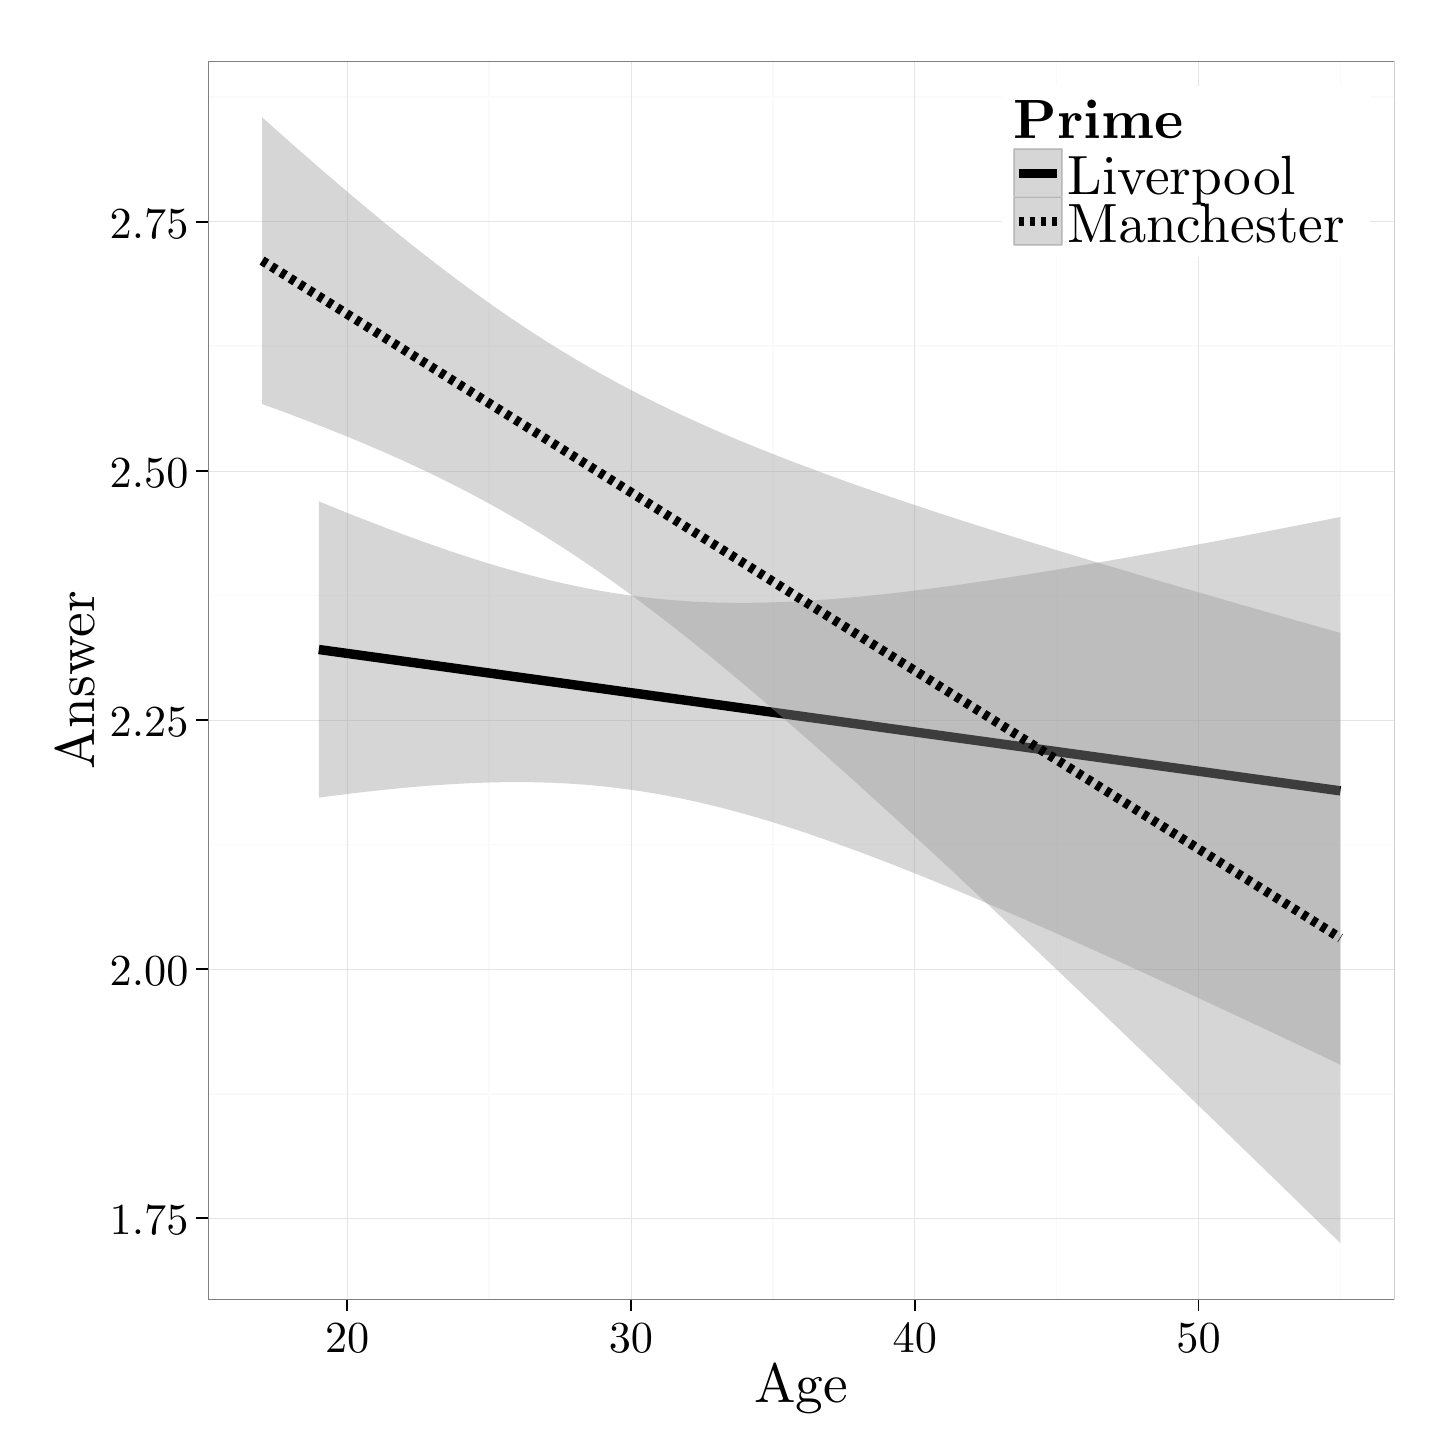
\begin{tikzpicture}[x=1pt,y=1pt]
\definecolor{fillColor}{RGB}{255,255,255}
\path[use as bounding box,fill=fillColor,fill opacity=0.00] (0,0) rectangle (505.89,505.89);
\begin{scope}
\path[clip] (  0.00,  0.00) rectangle (505.89,505.89);
\definecolor{drawColor}{RGB}{255,255,255}
\definecolor{fillColor}{RGB}{255,255,255}

\path[draw=drawColor,line width= 0.6pt,line join=round,line cap=round,fill=fillColor] (  0.00, -0.00) rectangle (505.89,505.89);
\end{scope}
\begin{scope}
\path[clip] ( 65.21, 46.31) rectangle (493.85,493.84);
\definecolor{fillColor}{RGB}{255,255,255}

\path[fill=fillColor] ( 65.21, 46.31) rectangle (493.85,493.84);
\definecolor{drawColor}{gray}{0.98}

\path[draw=drawColor,line width= 0.6pt,line join=round] ( 65.21,120.69) --
	(493.85,120.69);

\path[draw=drawColor,line width= 0.6pt,line join=round] ( 65.21,210.72) --
	(493.85,210.72);

\path[draw=drawColor,line width= 0.6pt,line join=round] ( 65.21,300.74) --
	(493.85,300.74);

\path[draw=drawColor,line width= 0.6pt,line join=round] ( 65.21,390.76) --
	(493.85,390.76);

\path[draw=drawColor,line width= 0.6pt,line join=round] ( 65.21,480.79) --
	(493.85,480.79);

\path[draw=drawColor,line width= 0.6pt,line join=round] (166.73, 46.31) --
	(166.73,493.84);

\path[draw=drawColor,line width= 0.6pt,line join=round] (269.28, 46.31) --
	(269.28,493.84);

\path[draw=drawColor,line width= 0.6pt,line join=round] (371.82, 46.31) --
	(371.82,493.84);

\path[draw=drawColor,line width= 0.6pt,line join=round] (474.36, 46.31) --
	(474.36,493.84);
\definecolor{drawColor}{gray}{0.90}

\path[draw=drawColor,line width= 0.2pt,line join=round] ( 65.21, 75.68) --
	(493.85, 75.68);

\path[draw=drawColor,line width= 0.2pt,line join=round] ( 65.21,165.70) --
	(493.85,165.70);

\path[draw=drawColor,line width= 0.2pt,line join=round] ( 65.21,255.73) --
	(493.85,255.73);

\path[draw=drawColor,line width= 0.2pt,line join=round] ( 65.21,345.75) --
	(493.85,345.75);

\path[draw=drawColor,line width= 0.2pt,line join=round] ( 65.21,435.77) --
	(493.85,435.77);

\path[draw=drawColor,line width= 0.2pt,line join=round] (115.46, 46.31) --
	(115.46,493.84);

\path[draw=drawColor,line width= 0.2pt,line join=round] (218.00, 46.31) --
	(218.00,493.84);

\path[draw=drawColor,line width= 0.2pt,line join=round] (320.55, 46.31) --
	(320.55,493.84);

\path[draw=drawColor,line width= 0.2pt,line join=round] (423.09, 46.31) --
	(423.09,493.84);
\definecolor{fillColor}{RGB}{153,153,153}

\path[fill=fillColor,fill opacity=0.40] (105.21,334.72) --
	(109.88,332.81) --
	(114.55,330.93) --
	(119.22,329.07) --
	(123.90,327.25) --
	(128.57,325.45) --
	(133.24,323.68) --
	(137.92,321.95) --
	(142.59,320.26) --
	(147.26,318.61) --
	(151.93,317.00) --
	(156.61,315.44) --
	(161.28,313.93) --
	(165.95,312.46) --
	(170.63,311.06) --
	(175.30,309.71) --
	(179.97,308.43) --
	(184.64,307.21) --
	(189.32,306.06) --
	(193.99,304.99) --
	(198.66,303.98) --
	(203.34,303.05) --
	(208.01,302.21) --
	(212.68,301.44) --
	(217.35,300.75) --
	(222.03,300.14) --
	(226.70,299.61) --
	(231.37,299.17) --
	(236.05,298.80) --
	(240.72,298.50) --
	(245.39,298.28) --
	(250.06,298.14) --
	(254.74,298.06) --
	(259.41,298.05) --
	(264.08,298.10) --
	(268.76,298.21) --
	(273.43,298.37) --
	(278.10,298.59) --
	(282.77,298.86) --
	(287.45,299.17) --
	(292.12,299.53) --
	(296.79,299.93) --
	(301.47,300.36) --
	(306.14,300.83) --
	(310.81,301.33) --
	(315.48,301.87) --
	(320.16,302.43) --
	(324.83,303.02) --
	(329.50,303.63) --
	(334.18,304.26) --
	(338.85,304.92) --
	(343.52,305.60) --
	(348.19,306.29) --
	(352.87,307.00) --
	(357.54,307.73) --
	(362.21,308.47) --
	(366.89,309.23) --
	(371.56,310.00) --
	(376.23,310.78) --
	(380.90,311.58) --
	(385.58,312.38) --
	(390.25,313.20) --
	(394.92,314.02) --
	(399.60,314.85) --
	(404.27,315.70) --
	(408.94,316.55) --
	(413.61,317.40) --
	(418.29,318.27) --
	(422.96,319.14) --
	(427.63,320.02) --
	(432.31,320.90) --
	(436.98,321.79) --
	(441.65,322.68) --
	(446.32,323.58) --
	(451.00,324.49) --
	(455.67,325.40) --
	(460.34,326.31) --
	(465.02,327.23) --
	(469.69,328.15) --
	(474.36,329.08) --
	(474.36,131.15) --
	(469.69,133.37) --
	(465.02,135.58) --
	(460.34,137.79) --
	(455.67,140.00) --
	(451.00,142.20) --
	(446.32,144.40) --
	(441.65,146.59) --
	(436.98,148.78) --
	(432.31,150.96) --
	(427.63,153.14) --
	(422.96,155.31) --
	(418.29,157.48) --
	(413.61,159.63) --
	(408.94,161.78) --
	(404.27,163.93) --
	(399.60,166.06) --
	(394.92,168.19) --
	(390.25,170.31) --
	(385.58,172.41) --
	(380.90,174.51) --
	(376.23,176.60) --
	(371.56,178.68) --
	(366.89,180.74) --
	(362.21,182.79) --
	(357.54,184.82) --
	(352.87,186.85) --
	(348.19,188.85) --
	(343.52,190.84) --
	(338.85,192.81) --
	(334.18,194.76) --
	(329.50,196.68) --
	(324.83,198.59) --
	(320.16,200.47) --
	(315.48,202.33) --
	(310.81,204.15) --
	(306.14,205.95) --
	(301.47,207.71) --
	(296.79,209.44) --
	(292.12,211.13) --
	(287.45,212.78) --
	(282.77,214.39) --
	(278.10,215.95) --
	(273.43,217.46) --
	(268.76,218.92) --
	(264.08,220.32) --
	(259.41,221.66) --
	(254.74,222.94) --
	(250.06,224.16) --
	(245.39,225.30) --
	(240.72,226.38) --
	(236.05,227.38) --
	(231.37,228.30) --
	(226.70,229.15) --
	(222.03,229.91) --
	(217.35,230.60) --
	(212.68,231.20) --
	(208.01,231.73) --
	(203.34,232.17) --
	(198.66,232.54) --
	(193.99,232.83) --
	(189.32,233.04) --
	(184.64,233.19) --
	(179.97,233.26) --
	(175.30,233.27) --
	(170.63,233.22) --
	(165.95,233.11) --
	(161.28,232.94) --
	(156.61,232.72) --
	(151.93,232.45) --
	(147.26,232.13) --
	(142.59,231.77) --
	(137.92,231.38) --
	(133.24,230.94) --
	(128.57,230.47) --
	(123.90,229.96) --
	(119.22,229.43) --
	(114.55,228.87) --
	(109.88,228.28) --
	(105.21,227.66) --
	cycle;
\definecolor{drawColor}{RGB}{0,0,0}

\path[draw=drawColor,line width= 3.4pt,line join=round] (105.21,281.19) --
	(109.88,280.54) --
	(114.55,279.90) --
	(119.22,279.25) --
	(123.90,278.60) --
	(128.57,277.96) --
	(133.24,277.31) --
	(137.92,276.66) --
	(142.59,276.02) --
	(147.26,275.37) --
	(151.93,274.73) --
	(156.61,274.08) --
	(161.28,273.43) --
	(165.95,272.79) --
	(170.63,272.14) --
	(175.30,271.49) --
	(179.97,270.85) --
	(184.64,270.20) --
	(189.32,269.55) --
	(193.99,268.91) --
	(198.66,268.26) --
	(203.34,267.61) --
	(208.01,266.97) --
	(212.68,266.32) --
	(217.35,265.67) --
	(222.03,265.03) --
	(226.70,264.38) --
	(231.37,263.73) --
	(236.05,263.09) --
	(240.72,262.44) --
	(245.39,261.79) --
	(250.06,261.15) --
	(254.74,260.50) --
	(259.41,259.85) --
	(264.08,259.21) --
	(268.76,258.56) --
	(273.43,257.91) --
	(278.10,257.27) --
	(282.77,256.62) --
	(287.45,255.98) --
	(292.12,255.33) --
	(296.79,254.68) --
	(301.47,254.04) --
	(306.14,253.39) --
	(310.81,252.74) --
	(315.48,252.10) --
	(320.16,251.45) --
	(324.83,250.80) --
	(329.50,250.16) --
	(334.18,249.51) --
	(338.85,248.86) --
	(343.52,248.22) --
	(348.19,247.57) --
	(352.87,246.92) --
	(357.54,246.28) --
	(362.21,245.63) --
	(366.89,244.98) --
	(371.56,244.34) --
	(376.23,243.69) --
	(380.90,243.04) --
	(385.58,242.40) --
	(390.25,241.75) --
	(394.92,241.10) --
	(399.60,240.46) --
	(404.27,239.81) --
	(408.94,239.16) --
	(413.61,238.52) --
	(418.29,237.87) --
	(422.96,237.23) --
	(427.63,236.58) --
	(432.31,235.93) --
	(436.98,235.29) --
	(441.65,234.64) --
	(446.32,233.99) --
	(451.00,233.35) --
	(455.67,232.70) --
	(460.34,232.05) --
	(465.02,231.41) --
	(469.69,230.76) --
	(474.36,230.11);

\path[fill=fillColor,fill opacity=0.40] ( 84.70,473.50) --
	( 89.63,469.10) --
	( 94.56,464.73) --
	( 99.49,460.40) --
	(104.43,456.10) --
	(109.36,451.84) --
	(114.29,447.63) --
	(119.22,443.46) --
	(124.16,439.34) --
	(129.09,435.27) --
	(134.02,431.26) --
	(138.95,427.31) --
	(143.89,423.43) --
	(148.82,419.62) --
	(153.75,415.87) --
	(158.68,412.21) --
	(163.62,408.62) --
	(168.55,405.12) --
	(173.48,401.70) --
	(178.41,398.38) --
	(183.35,395.14) --
	(188.28,391.99) --
	(193.21,388.94) --
	(198.14,385.97) --
	(203.08,383.10) --
	(208.01,380.32) --
	(212.94,377.62) --
	(217.87,375.01) --
	(222.81,372.47) --
	(227.74,370.02) --
	(232.67,367.63) --
	(237.60,365.32) --
	(242.54,363.07) --
	(247.47,360.88) --
	(252.40,358.74) --
	(257.33,356.66) --
	(262.27,354.63) --
	(267.20,352.65) --
	(272.13,350.71) --
	(277.06,348.81) --
	(282.00,346.95) --
	(286.93,345.12) --
	(291.86,343.32) --
	(296.79,341.55) --
	(301.73,339.81) --
	(306.66,338.09) --
	(311.59,336.40) --
	(316.52,334.72) --
	(321.46,333.07) --
	(326.39,331.44) --
	(331.32,329.82) --
	(336.25,328.22) --
	(341.19,326.64) --
	(346.12,325.07) --
	(351.05,323.51) --
	(355.98,321.97) --
	(360.92,320.43) --
	(365.85,318.91) --
	(370.78,317.40) --
	(375.71,315.90) --
	(380.64,314.40) --
	(385.58,312.92) --
	(390.51,311.44) --
	(395.44,309.97) --
	(400.37,308.50) --
	(405.31,307.05) --
	(410.24,305.59) --
	(415.17,304.15) --
	(420.10,302.71) --
	(425.04,301.28) --
	(429.97,299.85) --
	(434.90,298.42) --
	(439.83,297.00) --
	(444.77,295.59) --
	(449.70,294.18) --
	(454.63,292.77) --
	(459.56,291.36) --
	(464.50,289.96) --
	(469.43,288.57) --
	(474.36,287.17) --
	(474.36, 66.65) --
	(469.43, 71.45) --
	(464.50, 76.25) --
	(459.56, 81.05) --
	(454.63, 85.84) --
	(449.70, 90.63) --
	(444.77, 95.42) --
	(439.83,100.20) --
	(434.90,104.98) --
	(429.97,109.75) --
	(425.04,114.52) --
	(420.10,119.28) --
	(415.17,124.04) --
	(410.24,128.79) --
	(405.31,133.54) --
	(400.37,138.28) --
	(395.44,143.01) --
	(390.51,147.74) --
	(385.58,152.46) --
	(380.64,157.17) --
	(375.71,161.87) --
	(370.78,166.57) --
	(365.85,171.25) --
	(360.92,175.92) --
	(355.98,180.59) --
	(351.05,185.24) --
	(346.12,189.88) --
	(341.19,194.51) --
	(336.25,199.12) --
	(331.32,203.72) --
	(326.39,208.30) --
	(321.46,212.86) --
	(316.52,217.41) --
	(311.59,221.94) --
	(306.66,226.44) --
	(301.73,230.92) --
	(296.79,235.37) --
	(291.86,239.80) --
	(286.93,244.20) --
	(282.00,248.57) --
	(277.06,252.90) --
	(272.13,257.20) --
	(267.20,261.45) --
	(262.27,265.67) --
	(257.33,269.84) --
	(252.40,273.95) --
	(247.47,278.02) --
	(242.54,282.03) --
	(237.60,285.97) --
	(232.67,289.86) --
	(227.74,293.67) --
	(222.81,297.41) --
	(217.87,301.07) --
	(212.94,304.66) --
	(208.01,308.16) --
	(203.08,311.57) --
	(198.14,314.89) --
	(193.21,318.13) --
	(188.28,321.27) --
	(183.35,324.32) --
	(178.41,327.28) --
	(173.48,330.15) --
	(168.55,332.93) --
	(163.62,335.63) --
	(158.68,338.24) --
	(153.75,340.77) --
	(148.82,343.23) --
	(143.89,345.61) --
	(138.95,347.92) --
	(134.02,350.17) --
	(129.09,352.36) --
	(124.16,354.49) --
	(119.22,356.56) --
	(114.29,358.59) --
	(109.36,360.57) --
	(104.43,362.51) --
	( 99.49,364.41) --
	( 94.56,366.28) --
	( 89.63,368.11) --
	( 84.70,369.90) --
	cycle;

\path[draw=drawColor,line width= 3.4pt,dash pattern=on 2pt off 2pt ,line join=round] ( 84.70,421.70) --
	( 89.63,418.60) --
	( 94.56,415.51) --
	( 99.49,412.41) --
	(104.43,409.31) --
	(109.36,406.21) --
	(114.29,403.11) --
	(119.22,400.01) --
	(124.16,396.91) --
	(129.09,393.81) --
	(134.02,390.72) --
	(138.95,387.62) --
	(143.89,384.52) --
	(148.82,381.42) --
	(153.75,378.32) --
	(158.68,375.22) --
	(163.62,372.12) --
	(168.55,369.03) --
	(173.48,365.93) --
	(178.41,362.83) --
	(183.35,359.73) --
	(188.28,356.63) --
	(193.21,353.53) --
	(198.14,350.43) --
	(203.08,347.34) --
	(208.01,344.24) --
	(212.94,341.14) --
	(217.87,338.04) --
	(222.81,334.94) --
	(227.74,331.84) --
	(232.67,328.74) --
	(237.60,325.64) --
	(242.54,322.55) --
	(247.47,319.45) --
	(252.40,316.35) --
	(257.33,313.25) --
	(262.27,310.15) --
	(267.20,307.05) --
	(272.13,303.95) --
	(277.06,300.86) --
	(282.00,297.76) --
	(286.93,294.66) --
	(291.86,291.56) --
	(296.79,288.46) --
	(301.73,285.36) --
	(306.66,282.26) --
	(311.59,279.17) --
	(316.52,276.07) --
	(321.46,272.97) --
	(326.39,269.87) --
	(331.32,266.77) --
	(336.25,263.67) --
	(341.19,260.57) --
	(346.12,257.48) --
	(351.05,254.38) --
	(355.98,251.28) --
	(360.92,248.18) --
	(365.85,245.08) --
	(370.78,241.98) --
	(375.71,238.88) --
	(380.64,235.78) --
	(385.58,232.69) --
	(390.51,229.59) --
	(395.44,226.49) --
	(400.37,223.39) --
	(405.31,220.29) --
	(410.24,217.19) --
	(415.17,214.09) --
	(420.10,211.00) --
	(425.04,207.90) --
	(429.97,204.80) --
	(434.90,201.70) --
	(439.83,198.60) --
	(444.77,195.50) --
	(449.70,192.40) --
	(454.63,189.31) --
	(459.56,186.21) --
	(464.50,183.11) --
	(469.43,180.01) --
	(474.36,176.91);
\definecolor{drawColor}{gray}{0.50}

\path[draw=drawColor,line width= 0.6pt,line join=round,line cap=round] ( 65.21, 46.31) rectangle (493.85,493.84);
\end{scope}
\begin{scope}
\path[clip] (  0.00,  0.00) rectangle (505.89,505.89);
\definecolor{drawColor}{RGB}{0,0,0}

\node[text=drawColor,anchor=base east,inner sep=0pt, outer sep=0pt, scale=  1.60] at ( 58.10, 69.65) {1.75};

\node[text=drawColor,anchor=base east,inner sep=0pt, outer sep=0pt, scale=  1.60] at ( 58.10,159.67) {2.00};

\node[text=drawColor,anchor=base east,inner sep=0pt, outer sep=0pt, scale=  1.60] at ( 58.10,249.69) {2.25};

\node[text=drawColor,anchor=base east,inner sep=0pt, outer sep=0pt, scale=  1.60] at ( 58.10,339.72) {2.50};

\node[text=drawColor,anchor=base east,inner sep=0pt, outer sep=0pt, scale=  1.60] at ( 58.10,429.74) {2.75};
\end{scope}
\begin{scope}
\path[clip] (  0.00,  0.00) rectangle (505.89,505.89);
\definecolor{drawColor}{RGB}{0,0,0}

\path[draw=drawColor,line width= 0.6pt,line join=round] ( 60.95, 75.68) --
	( 65.21, 75.68);

\path[draw=drawColor,line width= 0.6pt,line join=round] ( 60.95,165.70) --
	( 65.21,165.70);

\path[draw=drawColor,line width= 0.6pt,line join=round] ( 60.95,255.73) --
	( 65.21,255.73);

\path[draw=drawColor,line width= 0.6pt,line join=round] ( 60.95,345.75) --
	( 65.21,345.75);

\path[draw=drawColor,line width= 0.6pt,line join=round] ( 60.95,435.77) --
	( 65.21,435.77);
\end{scope}
\begin{scope}
\path[clip] (  0.00,  0.00) rectangle (505.89,505.89);
\definecolor{drawColor}{RGB}{0,0,0}

\path[draw=drawColor,line width= 0.6pt,line join=round] (115.46, 42.04) --
	(115.46, 46.31);

\path[draw=drawColor,line width= 0.6pt,line join=round] (218.00, 42.04) --
	(218.00, 46.31);

\path[draw=drawColor,line width= 0.6pt,line join=round] (320.55, 42.04) --
	(320.55, 46.31);

\path[draw=drawColor,line width= 0.6pt,line join=round] (423.09, 42.04) --
	(423.09, 46.31);
\end{scope}
\begin{scope}
\path[clip] (  0.00,  0.00) rectangle (505.89,505.89);
\definecolor{drawColor}{RGB}{0,0,0}

\node[text=drawColor,anchor=base,inner sep=0pt, outer sep=0pt, scale=  1.60] at (115.46, 27.13) {20};

\node[text=drawColor,anchor=base,inner sep=0pt, outer sep=0pt, scale=  1.60] at (218.00, 27.13) {30};

\node[text=drawColor,anchor=base,inner sep=0pt, outer sep=0pt, scale=  1.60] at (320.55, 27.13) {40};

\node[text=drawColor,anchor=base,inner sep=0pt, outer sep=0pt, scale=  1.60] at (423.09, 27.13) {50};
\end{scope}
\begin{scope}
\path[clip] (  0.00,  0.00) rectangle (505.89,505.89);
\definecolor{drawColor}{RGB}{0,0,0}

\node[text=drawColor,anchor=base,inner sep=0pt, outer sep=0pt, scale=  2.00] at (279.53,  9.03) {Age};
\end{scope}
\begin{scope}
\path[clip] (  0.00,  0.00) rectangle (505.89,505.89);
\definecolor{drawColor}{RGB}{0,0,0}

\node[text=drawColor,rotate= 90.00,anchor=base,inner sep=0pt, outer sep=0pt, scale=  2.00] at ( 24.12,270.08) {Answer};
\end{scope}
\begin{scope}
\path[clip] (  0.00,  0.00) rectangle (505.89,505.89);
\definecolor{fillColor}{RGB}{255,255,255}

\path[fill=fillColor] (352.06,423.00) rectangle (484.98,484.98);
\end{scope}
\begin{scope}
\path[clip] (  0.00,  0.00) rectangle (505.89,505.89);
\definecolor{drawColor}{RGB}{0,0,0}

\node[text=drawColor,anchor=base west,inner sep=0pt, outer sep=0pt, scale=  2.00] at (356.32,465.96) {\bfseries Prime};
\end{scope}
\begin{scope}
\path[clip] (  0.00,  0.00) rectangle (505.89,505.89);
\definecolor{drawColor}{gray}{0.80}
\definecolor{fillColor}{RGB}{255,255,255}

\path[draw=drawColor,line width= 0.6pt,line join=round,line cap=round,fill=fillColor] (356.32,444.61) rectangle (373.67,461.96);
\end{scope}
\begin{scope}
\path[clip] (  0.00,  0.00) rectangle (505.89,505.89);
\definecolor{fillColor}{RGB}{153,153,153}

\path[fill=fillColor,fill opacity=0.40] (356.32,444.61) rectangle (373.67,461.96);
\definecolor{drawColor}{RGB}{0,0,0}

\path[draw=drawColor,line width= 3.4pt,line join=round] (358.06,453.29) -- (371.93,453.29);
\end{scope}
\begin{scope}
\path[clip] (  0.00,  0.00) rectangle (505.89,505.89);
\definecolor{drawColor}{gray}{0.80}
\definecolor{fillColor}{RGB}{255,255,255}

\path[draw=drawColor,line width= 0.6pt,line join=round,line cap=round,fill=fillColor] (356.32,427.27) rectangle (373.67,444.61);
\end{scope}
\begin{scope}
\path[clip] (  0.00,  0.00) rectangle (505.89,505.89);
\definecolor{fillColor}{RGB}{153,153,153}

\path[fill=fillColor,fill opacity=0.40] (356.32,427.27) rectangle (373.67,444.61);
\definecolor{drawColor}{RGB}{0,0,0}

\path[draw=drawColor,line width= 3.4pt,dash pattern=on 2pt off 2pt ,line join=round] (358.06,435.94) -- (371.93,435.94);
\end{scope}
\begin{scope}
\path[clip] (  0.00,  0.00) rectangle (505.89,505.89);
\definecolor{drawColor}{RGB}{0,0,0}

\node[text=drawColor,anchor=base west,inner sep=0pt, outer sep=0pt, scale=  2.00] at (375.84,445.75) {Liverpool};
\end{scope}
\begin{scope}
\path[clip] (  0.00,  0.00) rectangle (505.89,505.89);
\definecolor{drawColor}{RGB}{0,0,0}

\node[text=drawColor,anchor=base west,inner sep=0pt, outer sep=0pt, scale=  2.00] at (375.84,428.40) {Manchester};
\end{scope}
\end{tikzpicture}
} 
		\caption{/ŋ(g)/ (perception)  by age}
		\label{fig.scatter.ng.ext.age}
	\end{subfigure}
	\begin{subfigure}{.49\textwidth}
		\centering
			\definecolor{shadecolor}{rgb}{0.969, 0.969, 0.969}
			\resizebox{\linewidth}{!}{% Created by tikzDevice version 0.8.1 on 2016-02-09 02:19:13
% !TEX encoding = UTF-8 Unicode
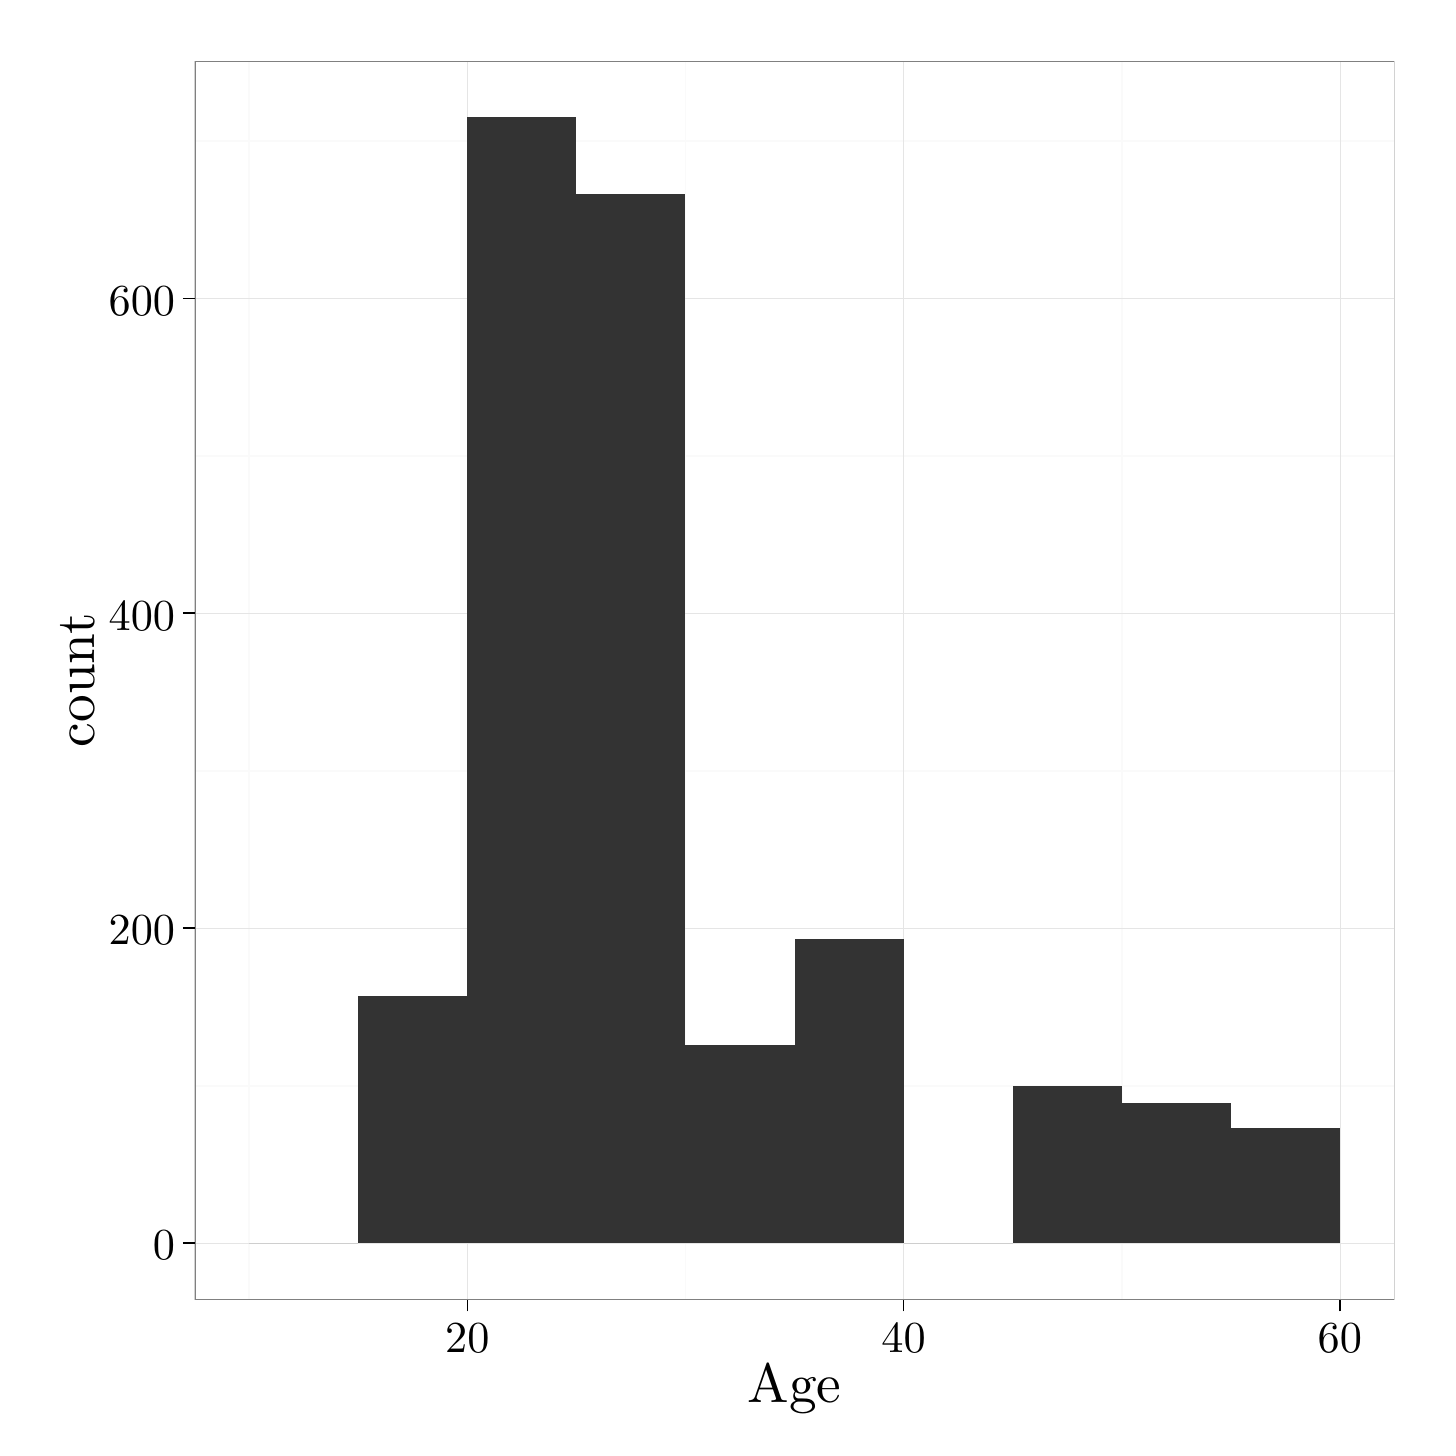
\begin{tikzpicture}[x=1pt,y=1pt]
\definecolor{fillColor}{RGB}{255,255,255}
\path[use as bounding box,fill=fillColor,fill opacity=0.00] (0,0) rectangle (505.89,505.89);
\begin{scope}
\path[clip] (  0.00,  0.00) rectangle (505.89,505.89);
\definecolor{drawColor}{RGB}{255,255,255}
\definecolor{fillColor}{RGB}{255,255,255}

\path[draw=drawColor,line width= 0.6pt,line join=round,line cap=round,fill=fillColor] (  0.00, -0.00) rectangle (505.89,505.89);
\end{scope}
\begin{scope}
\path[clip] ( 60.37, 46.31) rectangle (493.85,493.84);
\definecolor{fillColor}{RGB}{255,255,255}

\path[fill=fillColor] ( 60.37, 46.31) rectangle (493.85,493.84);
\definecolor{drawColor}{gray}{0.98}

\path[draw=drawColor,line width= 0.6pt,line join=round] ( 60.37,123.55) --
	(493.85,123.55);

\path[draw=drawColor,line width= 0.6pt,line join=round] ( 60.37,237.36) --
	(493.85,237.36);

\path[draw=drawColor,line width= 0.6pt,line join=round] ( 60.37,351.16) --
	(493.85,351.16);

\path[draw=drawColor,line width= 0.6pt,line join=round] ( 60.37,464.97) --
	(493.85,464.97);

\path[draw=drawColor,line width= 0.6pt,line join=round] ( 80.08, 46.31) --
	( 80.08,493.84);

\path[draw=drawColor,line width= 0.6pt,line join=round] (237.70, 46.31) --
	(237.70,493.84);

\path[draw=drawColor,line width= 0.6pt,line join=round] (395.33, 46.31) --
	(395.33,493.84);
\definecolor{drawColor}{gray}{0.90}

\path[draw=drawColor,line width= 0.2pt,line join=round] ( 60.37, 66.65) --
	(493.85, 66.65);

\path[draw=drawColor,line width= 0.2pt,line join=round] ( 60.37,180.45) --
	(493.85,180.45);

\path[draw=drawColor,line width= 0.2pt,line join=round] ( 60.37,294.26) --
	(493.85,294.26);

\path[draw=drawColor,line width= 0.2pt,line join=round] ( 60.37,408.06) --
	(493.85,408.06);

\path[draw=drawColor,line width= 0.2pt,line join=round] (158.89, 46.31) --
	(158.89,493.84);

\path[draw=drawColor,line width= 0.2pt,line join=round] (316.52, 46.31) --
	(316.52,493.84);

\path[draw=drawColor,line width= 0.2pt,line join=round] (474.14, 46.31) --
	(474.14,493.84);
\definecolor{fillColor}{gray}{0.20}

\path[fill=fillColor] ( 80.08, 66.65) rectangle (119.48, 66.65);

\path[fill=fillColor] (119.48, 66.65) rectangle (158.89,155.99);

\path[fill=fillColor] (158.89, 66.65) rectangle (198.30,473.50);

\path[fill=fillColor] (198.30, 66.65) rectangle (237.70,445.62);

\path[fill=fillColor] (237.70, 66.65) rectangle (277.11,138.35);

\path[fill=fillColor] (277.11, 66.65) rectangle (316.52,176.47);

\path[fill=fillColor] (316.52, 66.65) rectangle (355.92, 66.65);

\path[fill=fillColor] (355.92, 66.65) rectangle (395.33,123.55);

\path[fill=fillColor] (395.33, 66.65) rectangle (434.74,117.29);

\path[fill=fillColor] (434.74, 66.65) rectangle (474.14,108.19);
\definecolor{drawColor}{gray}{0.50}

\path[draw=drawColor,line width= 0.6pt,line join=round,line cap=round] ( 60.37, 46.31) rectangle (493.85,493.84);
\end{scope}
\begin{scope}
\path[clip] (  0.00,  0.00) rectangle (505.89,505.89);
\definecolor{drawColor}{RGB}{0,0,0}

\node[text=drawColor,anchor=base east,inner sep=0pt, outer sep=0pt, scale=  1.60] at ( 53.26, 60.62) {0};

\node[text=drawColor,anchor=base east,inner sep=0pt, outer sep=0pt, scale=  1.60] at ( 53.26,174.42) {200};

\node[text=drawColor,anchor=base east,inner sep=0pt, outer sep=0pt, scale=  1.60] at ( 53.26,288.23) {400};

\node[text=drawColor,anchor=base east,inner sep=0pt, outer sep=0pt, scale=  1.60] at ( 53.26,402.03) {600};
\end{scope}
\begin{scope}
\path[clip] (  0.00,  0.00) rectangle (505.89,505.89);
\definecolor{drawColor}{RGB}{0,0,0}

\path[draw=drawColor,line width= 0.6pt,line join=round] ( 56.10, 66.65) --
	( 60.37, 66.65);

\path[draw=drawColor,line width= 0.6pt,line join=round] ( 56.10,180.45) --
	( 60.37,180.45);

\path[draw=drawColor,line width= 0.6pt,line join=round] ( 56.10,294.26) --
	( 60.37,294.26);

\path[draw=drawColor,line width= 0.6pt,line join=round] ( 56.10,408.06) --
	( 60.37,408.06);
\end{scope}
\begin{scope}
\path[clip] (  0.00,  0.00) rectangle (505.89,505.89);
\definecolor{drawColor}{RGB}{0,0,0}

\path[draw=drawColor,line width= 0.6pt,line join=round] (158.89, 42.04) --
	(158.89, 46.31);

\path[draw=drawColor,line width= 0.6pt,line join=round] (316.52, 42.04) --
	(316.52, 46.31);

\path[draw=drawColor,line width= 0.6pt,line join=round] (474.14, 42.04) --
	(474.14, 46.31);
\end{scope}
\begin{scope}
\path[clip] (  0.00,  0.00) rectangle (505.89,505.89);
\definecolor{drawColor}{RGB}{0,0,0}

\node[text=drawColor,anchor=base,inner sep=0pt, outer sep=0pt, scale=  1.60] at (158.89, 27.13) {20};

\node[text=drawColor,anchor=base,inner sep=0pt, outer sep=0pt, scale=  1.60] at (316.52, 27.13) {40};

\node[text=drawColor,anchor=base,inner sep=0pt, outer sep=0pt, scale=  1.60] at (474.14, 27.13) {60};
\end{scope}
\begin{scope}
\path[clip] (  0.00,  0.00) rectangle (505.89,505.89);
\definecolor{drawColor}{RGB}{0,0,0}

\node[text=drawColor,anchor=base,inner sep=0pt, outer sep=0pt, scale=  2.00] at (277.11,  9.03) {Age};
\end{scope}
\begin{scope}
\path[clip] (  0.00,  0.00) rectangle (505.89,505.89);
\definecolor{drawColor}{RGB}{0,0,0}

\node[text=drawColor,rotate= 90.00,anchor=base,inner sep=0pt, outer sep=0pt, scale=  2.00] at ( 24.12,270.08) {count};
\end{scope}
\end{tikzpicture}
} 
		\caption{perception: age histogram}
		\label{fig.hist.ext.age}
	\end{subfigure}			
	\caption{Age in /ŋ(g)/ (perception) and overall}
\end{figure}

The last predictor that was found to be at least marginally significant (p = 0.089) in the mixed ordinal regression model for /ŋ(g)/ is age, the impact of which is visualised in Figure \ref{fig.scatter.ng.ext.age}, which shows age on the x-axis and estimated answer token on the y-axis, and codes \isi{priming} condition by line type.
Both regression lines have a downward slope, which was expected, given that the coefficient for age in the mixed-effects model was \ensuremath{-0.025}.
At first glance, subjects in different \isi{priming} conditions again seem to behave differently.
There is hardly any movement in the `\isi{Liverpool}' condition, the solid line is almost flat.
The dashed regression line for participants in the `\isi{Manchester}' condition, on the other hand, drops much more dramatically.
One might be tempted to conclude that \isi{priming} affected subjects of different ages in different ways.
If we consider the error ranges, however, it becomes clear that this would be an unwarranted deduction.
While it is true that the two regression lines are clearly separate for the youngest subjects in the sample (on the left hand side of the graph) and that they approach (and cross!) each other as we move along the age scale, it also has to be noted that both lines lie within a shared standard deviation\ once we reach participants aged around 37 and older.
This could simply be due to the fact that the sample is heavily skewed towards subjects in their twenties (cf. Figure \ref{fig.hist.ext.age}, which shows that the vast majority of observations stems from subjects that are between 20 and 30 years of age), but in any case there seems to be far too much noise in the answers given by older subjects to meaningfully speculate about any differences that might exist.
This is particularly true since the mixed-effects model does not contain a significant interaction of \isi{prime} and age.

\section{/k/}
\label{sec.perc_res.k}
	\subsection{Overview}
	\label{sec.perc_res.k.overview}

The condition number in the maximal model fit to responses relating to /k/ stimuli was slightly above the threshold for medium \isi{collinearity} (κ = 15.94), and, just as for velar nasal plus, this was due to a strong correlation of frequency and \isi{phonological environment}.
Another look at Table \ref{tab.keywords.frequency} on page \pageref{tab.keywords.frequency} reveals that if we compare keywords from the two phonological contexts in pairs (least frequent \_\# word and least frequent V\_V word, medium frequency \_\# word and medium frequency V\_V word, most frequent \_\# word and most frequent V\_V word), the \isi{Zipf} score of the keywords with the variable in \isi{word-final} position is always higher.
High frequency is thus, in this very limited sample, largely identical with \isi{word-final} occurrence of the variable.
Removing frequency as a fixed effect halved \isi{collinearity} in the maximal model (κ = 7.9).
Model selection based on AIC scores and F-tests comparing nested models resulted in the minimal adequate model printed below.

\begin{table}
	\caption{/k/ (perception): mixed-effects ordinal regression}
	\centering
	\begin{tabular}{p{0.2\textwidth}rrrrl}
		\hline
		Fixed effects: & Estimate & Std. Error & z value & Pr($>$$|$z$|$) & \\ 
		\hline
		Prime[\isi{Liverpool}] & 0.048 & 0.199 & 0.240 & 0.810 & \\ 
		ClassSubj[mc] & 0.622 & 0.200 & 3.110 & < 0.01 & **\\ 
		Environment[\_\#] & -0.391 & 0.104 & -3.764 & < 0.001 & ***\\ 
		Distance & 0.232 & 0.121 & 1.912 & 0.056 & .\\ 
		Prime[Liv.]:Class[mc] & -0.373 & 0.199 & -1.870 & 0.061 & .\\ 
		\hline
		Random effects: & & & & & \\
		Groups & Name & Variance & Std.Dev. & &  \\
		Questionnaire &  (Intercept) & 0.227 & 0.477 & &  \\
		Questionnaire & Token      & <0.001 & <0.001 & &  \\
		\multicolumn{3}{l}{(number of obs: 522, groups: Questionnaire, 55)} & & & \\
		\hline
	\end{tabular}
\end{table}

Prime is not among the significant predictors but this is only because the model found an interaction of \isi{prime} and \isi{social class} that almost reached significance and was therefore kept in the model.
When the interaction is removed \isi{prime} turns into a significant main effect (p = 0.046).
Social class, on the other hand, is (nearly) significant both as part of the interaction with \isi{prime} and as a main effect of its own.
The positive coefficient of 0.622 indicates that middle-class speakers tend to perceive higher-numbered tokens.
With a p-value below 0.001, \isi{phonological environment} is even more significant as a predictor than it was for /ŋ(g)/ answers.
The coefficient (\ensuremath{-0.391}), however, is negative, which indicates that \isi{word-final} /k/'s actually increase the likelihood of lower-numbered, i.e. more standard/\isi{Mancunian} tokens.
For velar nasal plus, the effect was in the opposite direction.
Geographical distance does not quite reach significance (p = 0.056), but the p-value is low enough to qualify as a statistical trend, so the factor was kept in the model\footnote{When \isi{Zipf} scores are kept in the maximal model despite the \isi{collinearity} with \isi{phonological environment}, the minimal adequate model one arrives at is not too different from the one printed above. Social class and \isi{phonological environment} remain significant predictors, but the interaction of \isi{prime} and \isi{social class} is eliminated from the model and, as a result, \isi{prime} alone is found to be a significant fixed effect. The p-value for \isi{geographical distance} is slightly greater than 0.1, so this factor gets eliminated. With a p-value of 0.113, the predictor frequency almost qualifies as a statistical trend. The impact of frequency will therefore be briefly analysed, too, in order to complete the picture.}.
I will now discuss these factors in more detail, starting once more with \isi{prime}.

\subsection{Prime and social class}
\label{sec.perc_res.k.prime}

\begin{figure}[h]
	\centering
		\definecolor{shadecolor}{rgb}{0.969, 0.969, 0.969}
		\resizebox{.49\linewidth}{!}{\input{figures/bar_k_ext-1.tikz}} 
	\caption{/k/ (perception) by prime}
	\label{fig.bar.k.tot.ext}
\end{figure}

Interestingly, there are a number of parallels in the pooled results for \textsc{nurse} and \isi{lenition} of /k/ as visualised in Figures \ref{fig.bar.nurse.tot.ext} and \ref{fig.bar.k.tot.ext} (\isi{remember} that the corresponding graphs for happ\textsc{y} and /ŋ(g)/ also resembled each other):
Again, the preference of subjects to choose the objectively most accurate token 2 is obvious in Figure \ref{fig.bar.k.tot.ext}: 70--75\% of answers belong to this category.
Token 1 (\isi{plosive} with burst, but no aspiration) accounts for 20\% of responses in the `\isi{Manchester}' group, and 30\% of answers for the participants who were primed for \isi{Liverpool}.
The \isi{affricate} (token 3) and \isi{fricative} (token 4) are rarely chosen across the board, but still clearly more often if people think the speaker is from \isi{Manchester} (light grey bars).
Once more, the \isi{priming} effect is not in the expected direction: Subjects are \emph{less} likely to perceive /k/-\isi{lenition} if they are led to believe the speaker is actually from \isi{Liverpool}.

In the \textsc{nurse} results there was also a sizeable proportion of token 3 (mild \isi{Scouse}) answers, which has `moved' to token 1 (hyper standard/\isi{Mancunian}) in the responses to /k/ stimuli.
Apart from that, pooled results for the two \isi{salient} variables are remarkably similar: pronounced preference for the objectively most accurate token in both conditions, \isi{priming} effect in the unexpected direction.
This \isi{priming} effect is subtle (people are not fooled most of the time and choose the `correct' token 2 in three out of four cases), but nevertheless clearly visible in the graph.
While \isi{prime} is not a significant main effect in the mixed ordinal regression model (due to the presence of the interaction with \isi{social class}, see beginning of this section), the difference between conditions is found to be significant in a model not including this interaction (estimate = -0.256, se = 0.128, z value = -1.999, p = 0.046), which supports the interpretation of Figure \ref{fig.bar.k.tot.ext} just presented.
The interaction of \isi{prime} and \isi{social class} is what we will look at next.

\begin{figure}[h]
	\centering
	\begin{subfigure}{0.49\textwidth}
		\centering
			\definecolor{shadecolor}{rgb}{0.969, 0.969, 0.969}
			\resizebox{\linewidth}{!}{\input{figures/bar_k_ext_wc-1.tikz}} 
		\caption{working class}
		\label{fig.bar.k.ext.wc}
	\end{subfigure}
	\begin{subfigure}{0.49\textwidth}
		\centering
			\definecolor{shadecolor}{rgb}{0.969, 0.969, 0.969}
			\resizebox{\linewidth}{!}{\input{figures/bar_k_ext_mc-1.tikz}} 
		\caption{middle class}
		\label{fig.bar.k.ext.mc}
	\end{subfigure}
	\caption{/k/ (perception) by social class}
	\label{fig.bar.k.ext.class}
\end{figure}

Figure \ref{fig.bar.k.ext.wc} shows the data for working-class subjects only, while Figure \ref{fig.bar.k.ext.mc} visualises the responses given by middle-class participants.
As outlined earlier, the correlation coefficient calculated by the mixed-effects model for middle class (0.622) suggests that middle-class participants were more likely to perceive higher-numbered tokens.
The two subplots of Figure \ref{fig.bar.k.ext.class} illustrate this in an impressively (and unexpectedly) clear way.
working-class participants chose answer token 1 in around 45\% and token 2 in about 55\% of cases when they were in the `\isi{Liverpool}' condition; the WC subjects in the `\isi{Manchester}' condition reverse these figures.
Two factors are responsible for the lower average of WC subjects:
\begin{inparaenum}[(a)]
	\item Working-class participants never (!) chose tokens 3 or 4 (irrespective of \isi{priming} condition), and
	\item tokens 1 and 2 have an (almost, if conditions are considered separately) equal share of the total number of WC answers.
\end{inparaenum} 

Middle-class subjects, on the other hand, show a distribution which is very similar to the one we find when results are pooled for \isi{social class} (cf. Figure \ref{fig.bar.k.tot.ext}).
This is not surprising, given that subjects with a middle-class background clearly dominate the sample in terms of numbers (cf. Section \ref{sec.perc_method.subjects}).
Token 2 accounts for 70--75\% of answers, depending on \isi{priming} condition.
Just as in Figure \ref{fig.bar.k.tot.ext}, the next most frequent answer is the hyper-standard/\isi{Mancunian} token number 1 (\isi{plosive} with burst, but no friction), which was chosen in around 25\% (`\isi{Liverpool}') and about 17\% (`\isi{Manchester}') of cases.
The \isi{affricate} (token 3) and \isi{fricative} variants (token 4) were once more only chosen in a small minority of cases, but clearly more often when subjects were primed for \isi{Manchester}.
The interaction of \isi{prime} and class that the mixed ordinal regression model found is thus also visible in the raw data.

\begin{figure}[h]
	\centering
		\definecolor{shadecolor}{rgb}{0.969, 0.969, 0.969}
		\resizebox{.49\linewidth}{!}{% Created by tikzDevice version 0.8.1 on 2016-02-09 02:19:38
% !TEX encoding = UTF-8 Unicode
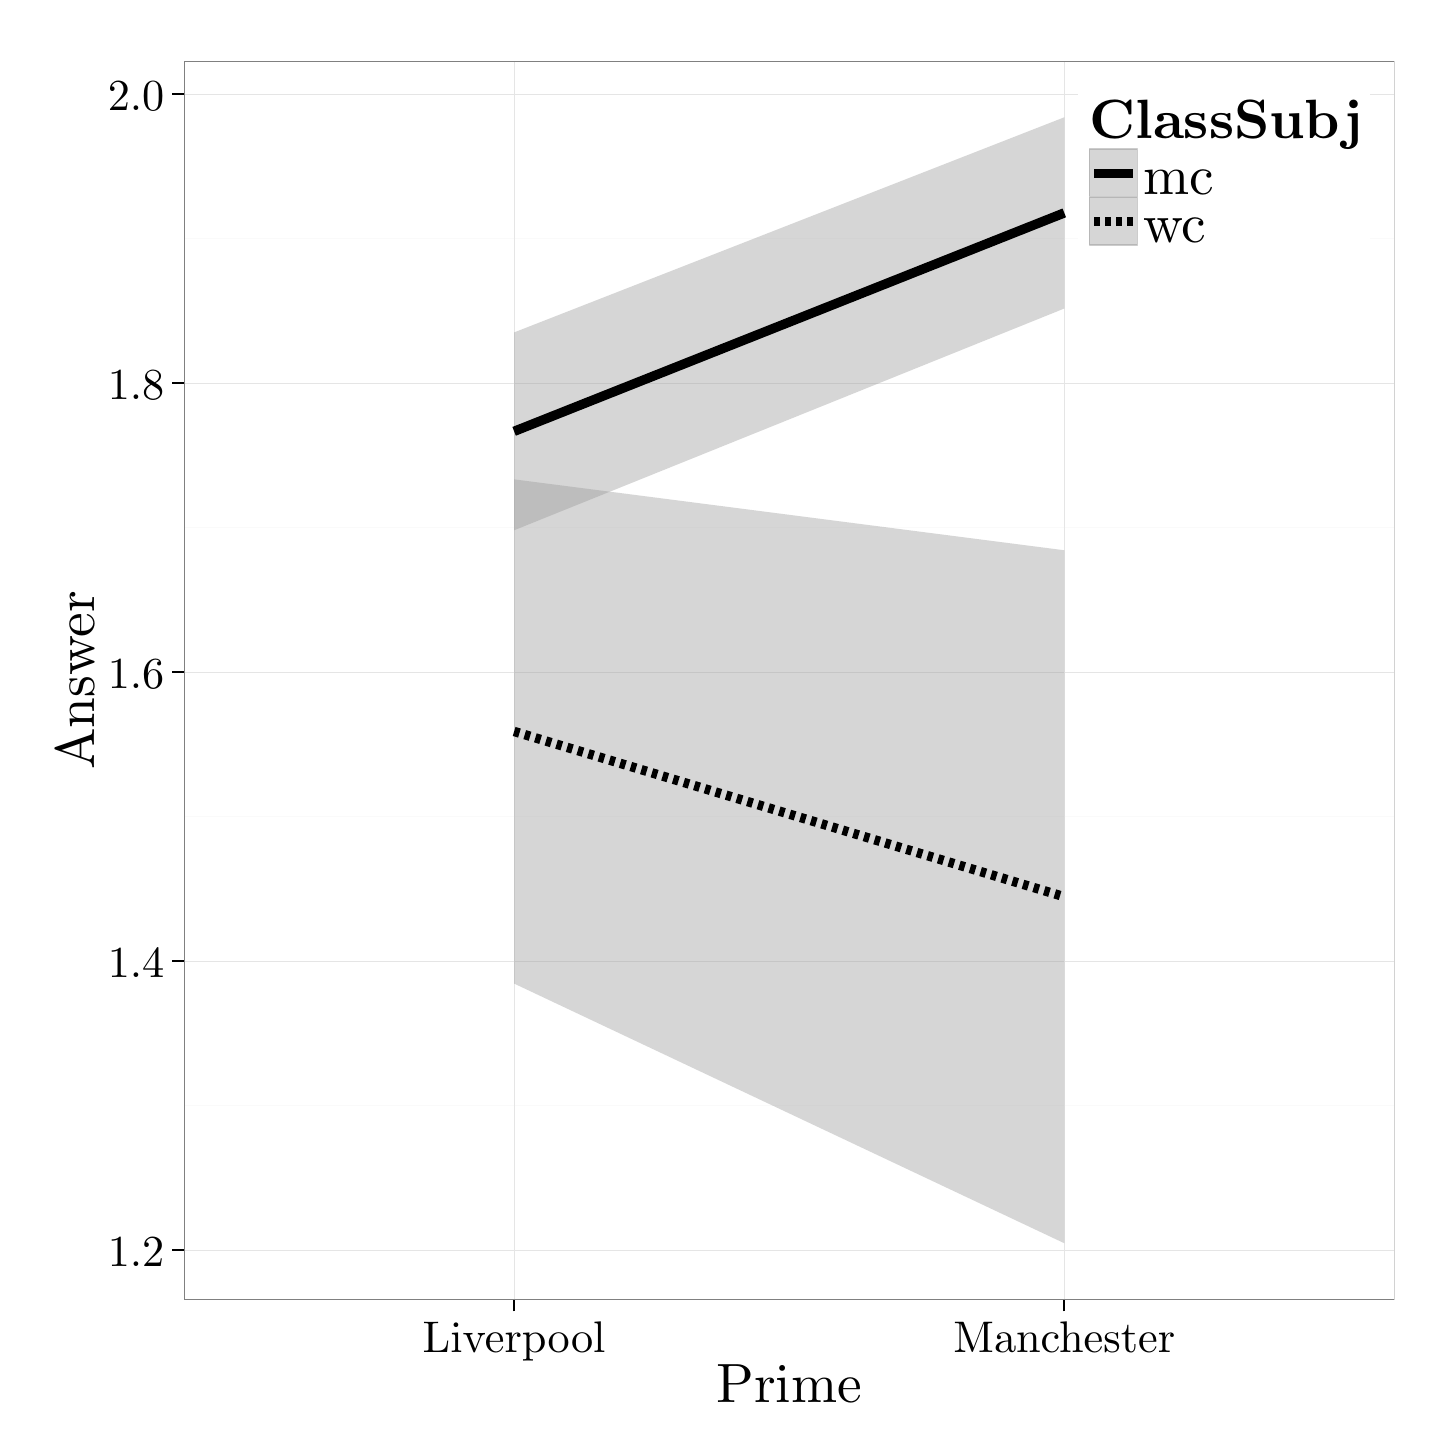
\begin{tikzpicture}[x=1pt,y=1pt]
\definecolor{fillColor}{RGB}{255,255,255}
\path[use as bounding box,fill=fillColor,fill opacity=0.00] (0,0) rectangle (505.89,505.89);
\begin{scope}
\path[clip] (  0.00,  0.00) rectangle (505.89,505.89);
\definecolor{drawColor}{RGB}{255,255,255}
\definecolor{fillColor}{RGB}{255,255,255}

\path[draw=drawColor,line width= 0.6pt,line join=round,line cap=round,fill=fillColor] (  0.00, -0.00) rectangle (505.89,505.89);
\end{scope}
\begin{scope}
\path[clip] ( 56.50, 46.31) rectangle (493.85,493.84);
\definecolor{fillColor}{RGB}{255,255,255}

\path[fill=fillColor] ( 56.50, 46.31) rectangle (493.85,493.84);
\definecolor{drawColor}{gray}{0.98}

\path[draw=drawColor,line width= 0.6pt,line join=round] ( 56.50,116.43) --
	(493.85,116.43);

\path[draw=drawColor,line width= 0.6pt,line join=round] ( 56.50,220.86) --
	(493.85,220.86);

\path[draw=drawColor,line width= 0.6pt,line join=round] ( 56.50,325.28) --
	(493.85,325.28);

\path[draw=drawColor,line width= 0.6pt,line join=round] ( 56.50,429.71) --
	(493.85,429.71);
\definecolor{drawColor}{gray}{0.90}

\path[draw=drawColor,line width= 0.2pt,line join=round] ( 56.50, 64.22) --
	(493.85, 64.22);

\path[draw=drawColor,line width= 0.2pt,line join=round] ( 56.50,168.64) --
	(493.85,168.64);

\path[draw=drawColor,line width= 0.2pt,line join=round] ( 56.50,273.07) --
	(493.85,273.07);

\path[draw=drawColor,line width= 0.2pt,line join=round] ( 56.50,377.50) --
	(493.85,377.50);

\path[draw=drawColor,line width= 0.2pt,line join=round] ( 56.50,481.92) --
	(493.85,481.92);

\path[draw=drawColor,line width= 0.2pt,line join=round] (175.78, 46.31) --
	(175.78,493.84);

\path[draw=drawColor,line width= 0.2pt,line join=round] (374.57, 46.31) --
	(374.57,493.84);
\definecolor{fillColor}{RGB}{153,153,153}

\path[fill=fillColor,fill opacity=0.40] (175.78,395.77) --
	(374.57,473.50) --
	(374.57,404.40) --
	(175.78,324.27) --
	cycle;
\definecolor{drawColor}{RGB}{0,0,0}

\path[draw=drawColor,line width= 3.4pt,line join=round] (175.78,360.02) --
	(374.57,438.95);

\path[fill=fillColor,fill opacity=0.40] (175.78,342.67) --
	(374.57,317.05) --
	(374.57, 66.65) --
	(175.78,160.47) --
	cycle;

\path[draw=drawColor,line width= 3.4pt,dash pattern=on 2pt off 2pt ,line join=round] (175.78,251.57) --
	(374.57,191.85);
\definecolor{drawColor}{gray}{0.50}

\path[draw=drawColor,line width= 0.6pt,line join=round,line cap=round] ( 56.50, 46.31) rectangle (493.85,493.84);
\end{scope}
\begin{scope}
\path[clip] (  0.00,  0.00) rectangle (505.89,505.89);
\definecolor{drawColor}{RGB}{0,0,0}

\node[text=drawColor,anchor=base east,inner sep=0pt, outer sep=0pt, scale=  1.60] at ( 49.39, 58.18) {1.2};

\node[text=drawColor,anchor=base east,inner sep=0pt, outer sep=0pt, scale=  1.60] at ( 49.39,162.61) {1.4};

\node[text=drawColor,anchor=base east,inner sep=0pt, outer sep=0pt, scale=  1.60] at ( 49.39,267.04) {1.6};

\node[text=drawColor,anchor=base east,inner sep=0pt, outer sep=0pt, scale=  1.60] at ( 49.39,371.46) {1.8};

\node[text=drawColor,anchor=base east,inner sep=0pt, outer sep=0pt, scale=  1.60] at ( 49.39,475.89) {2.0};
\end{scope}
\begin{scope}
\path[clip] (  0.00,  0.00) rectangle (505.89,505.89);
\definecolor{drawColor}{RGB}{0,0,0}

\path[draw=drawColor,line width= 0.6pt,line join=round] ( 52.24, 64.22) --
	( 56.50, 64.22);

\path[draw=drawColor,line width= 0.6pt,line join=round] ( 52.24,168.64) --
	( 56.50,168.64);

\path[draw=drawColor,line width= 0.6pt,line join=round] ( 52.24,273.07) --
	( 56.50,273.07);

\path[draw=drawColor,line width= 0.6pt,line join=round] ( 52.24,377.50) --
	( 56.50,377.50);

\path[draw=drawColor,line width= 0.6pt,line join=round] ( 52.24,481.92) --
	( 56.50,481.92);
\end{scope}
\begin{scope}
\path[clip] (  0.00,  0.00) rectangle (505.89,505.89);
\definecolor{drawColor}{RGB}{0,0,0}

\path[draw=drawColor,line width= 0.6pt,line join=round] (175.78, 42.04) --
	(175.78, 46.31);

\path[draw=drawColor,line width= 0.6pt,line join=round] (374.57, 42.04) --
	(374.57, 46.31);
\end{scope}
\begin{scope}
\path[clip] (  0.00,  0.00) rectangle (505.89,505.89);
\definecolor{drawColor}{RGB}{0,0,0}

\node[text=drawColor,anchor=base,inner sep=0pt, outer sep=0pt, scale=  1.60] at (175.78, 27.13) {Liverpool};

\node[text=drawColor,anchor=base,inner sep=0pt, outer sep=0pt, scale=  1.60] at (374.57, 27.13) {Manchester};
\end{scope}
\begin{scope}
\path[clip] (  0.00,  0.00) rectangle (505.89,505.89);
\definecolor{drawColor}{RGB}{0,0,0}

\node[text=drawColor,anchor=base,inner sep=0pt, outer sep=0pt, scale=  2.00] at (275.17,  9.03) {Prime};
\end{scope}
\begin{scope}
\path[clip] (  0.00,  0.00) rectangle (505.89,505.89);
\definecolor{drawColor}{RGB}{0,0,0}

\node[text=drawColor,rotate= 90.00,anchor=base,inner sep=0pt, outer sep=0pt, scale=  2.00] at ( 24.12,270.08) {Answer};
\end{scope}
\begin{scope}
\path[clip] (  0.00,  0.00) rectangle (505.89,505.89);
\definecolor{fillColor}{RGB}{255,255,255}

\path[fill=fillColor] (379.38,423.00) rectangle (484.98,484.98);
\end{scope}
\begin{scope}
\path[clip] (  0.00,  0.00) rectangle (505.89,505.89);
\definecolor{drawColor}{RGB}{0,0,0}

\node[text=drawColor,anchor=base west,inner sep=0pt, outer sep=0pt, scale=  2.00] at (383.65,465.96) {\bfseries ClassSubj};
\end{scope}
\begin{scope}
\path[clip] (  0.00,  0.00) rectangle (505.89,505.89);
\definecolor{drawColor}{gray}{0.80}
\definecolor{fillColor}{RGB}{255,255,255}

\path[draw=drawColor,line width= 0.6pt,line join=round,line cap=round,fill=fillColor] (383.65,444.61) rectangle (400.99,461.96);
\end{scope}
\begin{scope}
\path[clip] (  0.00,  0.00) rectangle (505.89,505.89);
\definecolor{fillColor}{RGB}{153,153,153}

\path[fill=fillColor,fill opacity=0.40] (383.65,444.61) rectangle (400.99,461.96);
\definecolor{drawColor}{RGB}{0,0,0}

\path[draw=drawColor,line width= 3.4pt,line join=round] (385.38,453.29) -- (399.26,453.29);
\end{scope}
\begin{scope}
\path[clip] (  0.00,  0.00) rectangle (505.89,505.89);
\definecolor{drawColor}{gray}{0.80}
\definecolor{fillColor}{RGB}{255,255,255}

\path[draw=drawColor,line width= 0.6pt,line join=round,line cap=round,fill=fillColor] (383.65,427.27) rectangle (400.99,444.61);
\end{scope}
\begin{scope}
\path[clip] (  0.00,  0.00) rectangle (505.89,505.89);
\definecolor{fillColor}{RGB}{153,153,153}

\path[fill=fillColor,fill opacity=0.40] (383.65,427.27) rectangle (400.99,444.61);
\definecolor{drawColor}{RGB}{0,0,0}

\path[draw=drawColor,line width= 3.4pt,dash pattern=on 2pt off 2pt ,line join=round] (385.38,435.94) -- (399.26,435.94);
\end{scope}
\begin{scope}
\path[clip] (  0.00,  0.00) rectangle (505.89,505.89);
\definecolor{drawColor}{RGB}{0,0,0}

\node[text=drawColor,anchor=base west,inner sep=0pt, outer sep=0pt, scale=  2.00] at (403.16,445.75) {mc};
\end{scope}
\begin{scope}
\path[clip] (  0.00,  0.00) rectangle (505.89,505.89);
\definecolor{drawColor}{RGB}{0,0,0}

\node[text=drawColor,anchor=base west,inner sep=0pt, outer sep=0pt, scale=  2.00] at (403.16,428.40) {wc};
\end{scope}
\end{tikzpicture}
} 
	\caption{/k/ (perception) by prime and social class}
	\label{fig.scatter.k.ext.classprime}
\end{figure}

In Figure \ref{fig.scatter.k.ext.classprime} the interaction of these two factors is visualised.
As with the other scatter/regression plots estimated answer token is to be found on the y-axis.
On the x-axis we have the distinction into subjects primed for `\isi{Manchester}' and `\isi{Liverpool}'.
Social class, finally, is coded by line type: The solid line represents middle-class subjects, while the dashed line stands for working-class participants.
The difference between the two social classes is quite obvious.
For working-class subjects the regression line has a negative slope.
Average answer token number is lower in the `\isi{Manchester}' condition, so if there was a statistically significant \isi{priming} effect in this sub-group it would actually be in the expected direction (more Liverpool-like percepts in the `\isi{Liverpool}' condition, more Manchester-like percepts in the `\isi{Manchester}' condition).
In the middle-class group, this effect is reversed.
The positive slope indicates that participants who were primed for \isi{Liverpool} are \emph{less} likely to perceive \isi{Liverpool} variants of /k/.
The increase in the middle-class group is also steeper than the decrease in the working-class subjects, which suggests that there is more of an effect in the former than in the latter.
We also see that there seems to be much more variation in the answers given by working-class respondents (the standard error, marked by the grey area around the regression line, is much larger than the one for middle-class participants).
This is probably mostly due to the small number of observations in this sub-sample (n(WC) = 69; n(MC) = 487), which might also be the main reason why the difference is not statistically significant.

Since there is this very pronounced middle-class bias in the sample of this experiment (48 middle-class and 7 working-class subjects; 3 participants did not give their \isi{social class}), any conclusions drawn about \isi{social class} differences should be taken with a grain of salt.
Notwithstanding this caveat, it is highly interesting that a \isi{priming} effect can only be found for middle-class subjects, but not for their working-class counterparts.
Also, it remains striking, even if the small number of observations is taken into account, that WC subjects did not choose tokens 3 and 4 even once.
2.2\% (`\isi{Liverpool}') to 6.5\% (`\isi{Manchester}') of MC answers were token 3 or 4.
If working-class participants had similar percentages, tokens 3 and 4 would have been chosen between 1 and 5 times.
Furthermore, this result --- statistically shaky as it may be --- is in line with previous research.
\textcite{hayetal2006a} and \textcite{haydrager2010} both found an interaction of \isi{social class} and condition, and in both cases the \isi{priming} effect was most pronounced for the highest social classes, less extreme in the middle range, and completely absent for participants situated towards the lower end of the socioeconomic scale.

For a socially \isi{salient} variable, this should not really come as a surprise.
Rather, a result like this is only to be expected, because speakers from higher socioeconomic classes are, on the whole, hypothesised to be much more sensitive to, and aware of, social differences in language use.
It seems only logical that they would also be more susceptible to a manipulation that is based on these subtle differences.
Another option is that due to differences in mobility and social networks, working-class subjects just do not have any exemplars indexed with `\isi{Liverpool}' (the same would hold true for `\isi{Manchester}'), so \isi{priming} them cannot activate any exemplars that would bias their perception.

\subsection{Phonological context}
\label{sec.perc_res.k.phon}

The last (highly) significant factor in the mixed ordinal regression model is \isi{phonological environment}.
We have the same two environments \_\# and V\_V as for velar nasal plus.
Results for V\_V are visualised in Figure \ref{fig.bar.k.ext.intervoc}, those for \_\# contexts are represented by Figure \ref{fig.bar.k.ext.wordfinal}.
Similar to the results for /ŋ(g)/, where \isi{phonological context} was also a significant factor, there do not seem to be huge differences between Figures \ref{fig.bar.k.ext.intervoc} and \ref{fig.bar.k.ext.wordfinal}.
In both contexts, subjects show the clear preference for token 2 (released \isi{plosive} with normal aspiration) that we have already seen for the pooled results.
Token 1 (\isi{plosive} with burst, but no aspiration) is the next most frequent choice in both environments.
However, it accounts for between 15 and just above 20\% of answers in the \isi{intervocalic} stimuli, whereas for keywords that have the variable in \isi{word-final} position, token 1 is chosen in around 27 to 35\% of cases.
Tokens 3 (\isi{affricate}) and 4 (\isi{fricative}) have about the same share in both phonological contexts.
The fact that token 1 is a considerably more (and token 2 a considerably less) frequent response to \isi{word-final} stimuli thus explains why the mixed-effects model found a lower likelihood of higher-numbered answer tokens in this sub-sample (the coefficient is \ensuremath{-0.391}).

\begin{figure}[h]
	\centering
	\begin{subfigure}{0.49\textwidth}
		\centering
			\definecolor{shadecolor}{rgb}{0.969, 0.969, 0.969}
			\resizebox{\linewidth}{!}{\input{figures/bar_k_ext_intervoc-1.tikz}} 
		\caption{intervocalic}
		\label{fig.bar.k.ext.intervoc}
	\end{subfigure}
	\begin{subfigure}{0.49\textwidth}
		\centering
			\definecolor{shadecolor}{rgb}{0.969, 0.969, 0.969}
			\resizebox{\linewidth}{!}{\input{figures/bar_k_ext_wordfinal-1.tikz}}
		\caption{word-final}
		\label{fig.bar.k.ext.wordfinal}
	\end{subfigure}
	\caption{/k/ (perception) by environment}
	\label{fig.bar.k.ext.environment}
\end{figure}

One might also suspect a different size of the \isi{priming} effect when only looking at the two graphs.
Differences between conditions appear to be more pronounced in Figure \ref{fig.bar.k.ext.wordfinal}, particularly for token 2.
On the other hand, the potential influence of \isi{prime} seems to be largely identical in size for tokens 3 and 4 in both phonological contexts, and the distance between conditions for token 1 \emph{is} greater in \isi{word-final} than in \isi{intervocalic} environments, but not as much as it is for token 2.
If \isi{phonological context} does affect the degree of the \isi{priming} effect, then the difference can only be a very subtle one.
The raw data thus seem to support the fact that the mixed-effects model did not find a significant interaction of \isi{prime} and \isi{phonological environment}; the effect is largely the same.

Even though environments are not significantly different from each other, it is tempting to link the slightly more pronounced difference between \isi{priming} conditions for the \isi{word-final} stimuli to higher \isi{salience} of /k/-\isi{lenition} in this context.
Remember that, in production, subjects used more \isi{lenition} for /k/'s that appeared \isi{intervocalically} compared to those that occurred word-finally (cf. \ref{sec.prod.res.con.k.phon}).
This was taken to be a hint that \isi{lenition} of /k/ is more socially \isi{salient} in the latter environment, or, rather, it is \emph{less} \isi{salient} in \isi{intervocalic} contexts, possibly because leniting a stop in-between vowels can be `justified' phonetically (and is quite common typologically).
It would tie in nicely with the main hypothesis of this study if a feature that has been shown to be more \isi{salient} in a particular \isi{phonological environment} in production also creates a larger \isi{priming} effect in this context in perception.
Unfortunately, however, there is only little statistical evidence to support this claim, as has been pointed out above.

With respect to the stronger preference for token 2 in \isi{intervocalic} stimuli, there is a possible explanation that is more directly based on the \isi{phonological environment} itself, and one that also works for the significant difference between phonological contexts as a whole --- across \isi{priming} conditions --- that was revealed in the mixed ordinal regression.
In RP, GA, and many other accents of English, the \isi{voiceless} plosives /p, t, k/ have three main allophones which are in complementary distribution: Aspirated variants [pʰ, tʰ, kʰ] occur in simple onsets of syllables, unaspirated variants [p, t, k] are found in complex onsets, and \isi{unreleased} realisations [p̚, t̚, k̚~] are common in coda position.
For any \isi{word-final} /k/ stimulus it is therefore possible that subjects sub-\isi{consciously} expected a [k̚~] realisation.
In \isi{intervocalic}, i.e. syllable-initial position, on the other hand, the expected variant would be [kʰ].
Token 2 (\isi{plosive} with burst and aspiration, i.e. [kʰ]) thus fits expectations based on \isi{allophonic} distributions very well when /k/ is presented in inter-\isi{vocalic} environments.
If we assume that participants are somewhat biased to perceive a non-released [k̚~] in \isi{word-final} contexts, their best option to report this \isi{percept} would be choosing token 1 (\isi{plosive} with a short burst, but no aspiration) as it is phonetically most similar to [k̚~], so we would expect a larger share of token 1 answers, and this is exactly what we are seeing in Figures \ref{fig.bar.k.ext.intervoc} and \ref{fig.bar.k.ext.wordfinal}.
Explaining the larger proportion of token 1 answers for \_\# stimuli with expectations based on well-known \isi{allophonic} distributions is the same as saying subjects were primed by the \isi{phonological context}.
While there was no significant interaction of \isi{prime} and \isi{phonological environment} (differences between conditions are non-significant in both cases), then, we seem to have revealed an unintended \isi{priming} effect of \isi{phonological context} itself.

\subsection{Geographical distance}
\label{sec.perc_res.k.geography}

Let us now turn to \isi{geographical distance} from \isi{Liverpool}, a fixed effect which was not found to be significant in the mixed ordinal regression model, but whose p-value was low enough (p = 0.056) to qualify as a statistical trend.
The estimate found (0.232) suggests that higher-numbered answer tokens increase in parallel with growing distance from \isi{Liverpool}.
This trend is immediately obvious in Figure \ref{fig.scatter.k.ext.dist}.
As usual, the estimated answer token is marked on the y-axis.
On the x-axis we find Euclidean distance from \isi{Liverpool}, and \isi{priming} condition is once more coded by line type (dashed for `\isi{Manchester}', solid for `\isi{Liverpool}').

\begin{figure}[h]
	\centering
		\definecolor{shadecolor}{rgb}{0.969, 0.969, 0.969}
		\resizebox{.49\linewidth}{!}{% Created by tikzDevice version 0.8.1 on 2016-02-09 02:19:49
% !TEX encoding = UTF-8 Unicode
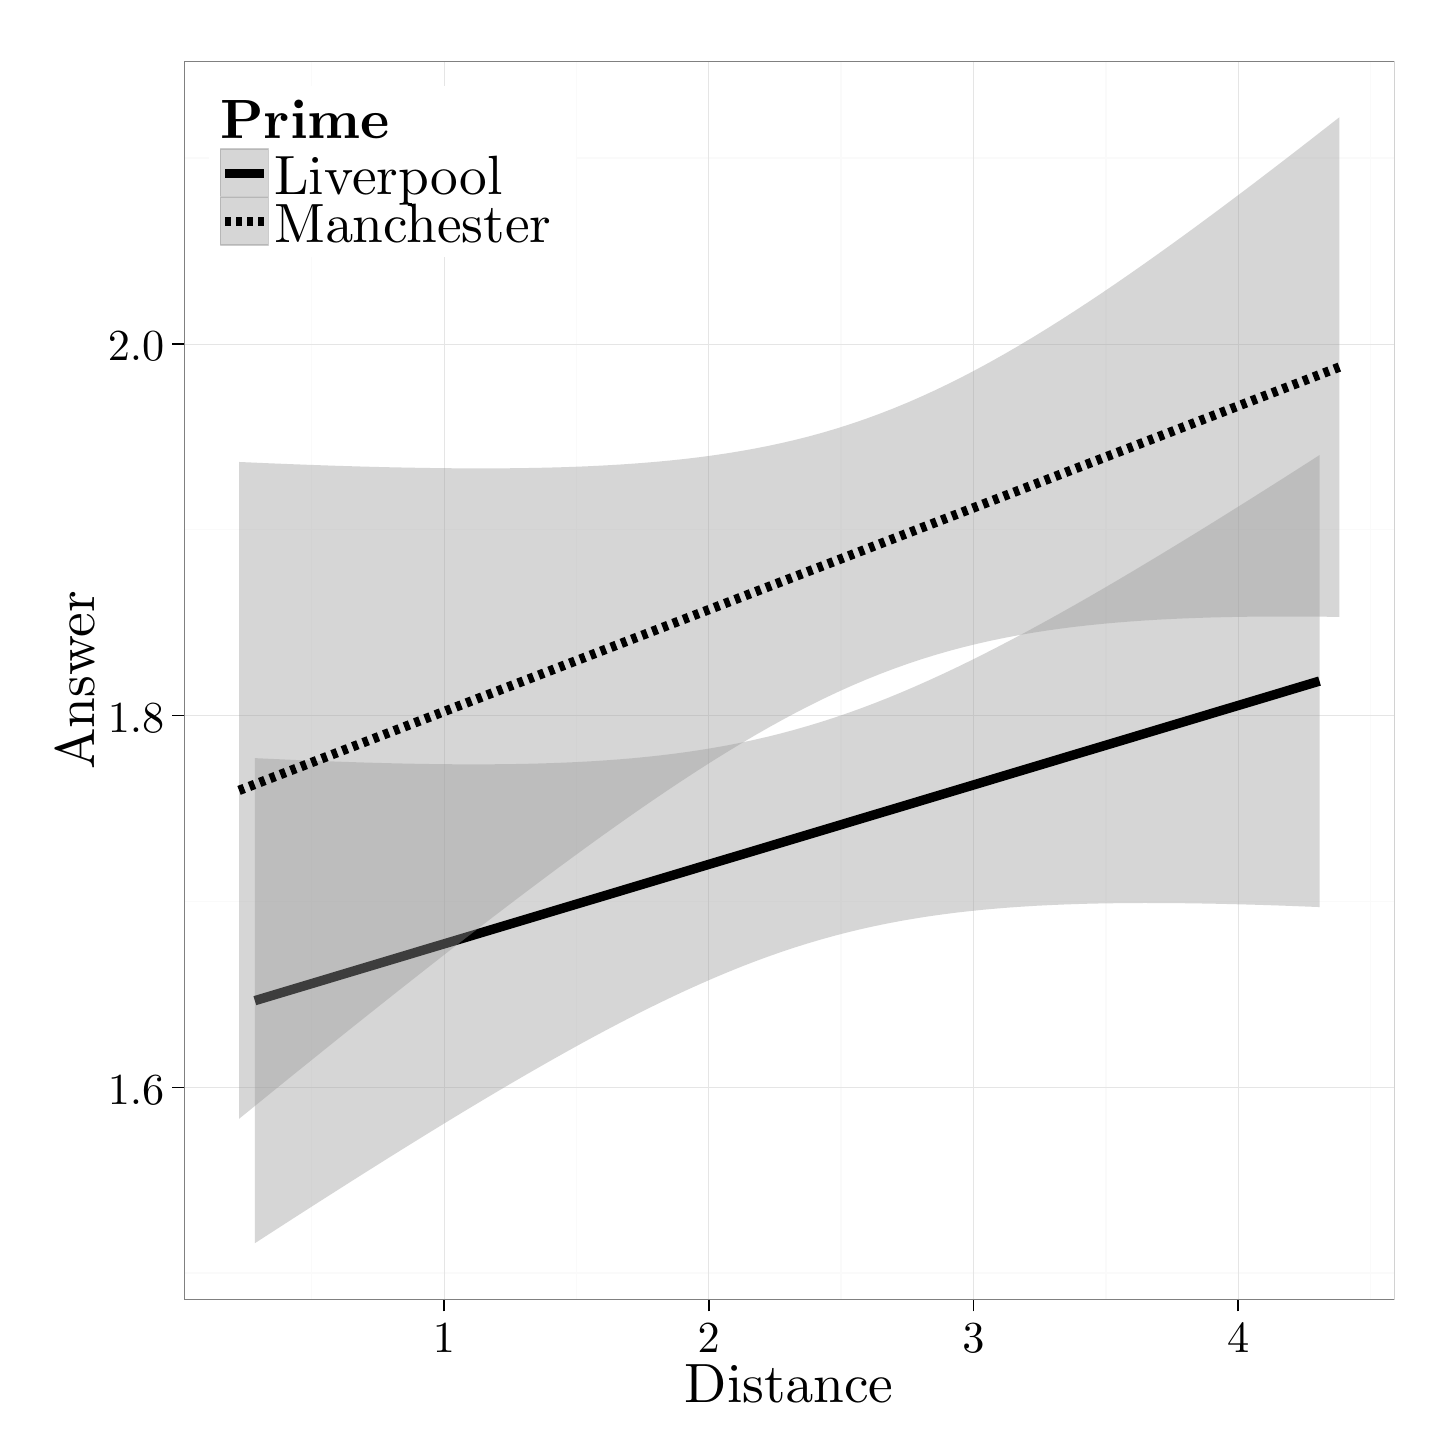
\begin{tikzpicture}[x=1pt,y=1pt]
\definecolor{fillColor}{RGB}{255,255,255}
\path[use as bounding box,fill=fillColor,fill opacity=0.00] (0,0) rectangle (505.89,505.89);
\begin{scope}
\path[clip] (  0.00,  0.00) rectangle (505.89,505.89);
\definecolor{drawColor}{RGB}{255,255,255}
\definecolor{fillColor}{RGB}{255,255,255}

\path[draw=drawColor,line width= 0.6pt,line join=round,line cap=round,fill=fillColor] (  0.00, -0.00) rectangle (505.89,505.89);
\end{scope}
\begin{scope}
\path[clip] ( 56.50, 46.31) rectangle (493.85,493.84);
\definecolor{fillColor}{RGB}{255,255,255}

\path[fill=fillColor] ( 56.50, 46.31) rectangle (493.85,493.84);
\definecolor{drawColor}{gray}{0.98}

\path[draw=drawColor,line width= 0.6pt,line join=round] ( 56.50, 55.80) --
	(493.85, 55.80);

\path[draw=drawColor,line width= 0.6pt,line join=round] ( 56.50,190.15) --
	(493.85,190.15);

\path[draw=drawColor,line width= 0.6pt,line join=round] ( 56.50,324.49) --
	(493.85,324.49);

\path[draw=drawColor,line width= 0.6pt,line join=round] ( 56.50,458.83) --
	(493.85,458.83);

\path[draw=drawColor,line width= 0.6pt,line join=round] (102.60, 46.31) --
	(102.60,493.84);

\path[draw=drawColor,line width= 0.6pt,line join=round] (198.27, 46.31) --
	(198.27,493.84);

\path[draw=drawColor,line width= 0.6pt,line join=round] (293.93, 46.31) --
	(293.93,493.84);

\path[draw=drawColor,line width= 0.6pt,line join=round] (389.60, 46.31) --
	(389.60,493.84);

\path[draw=drawColor,line width= 0.6pt,line join=round] (485.26, 46.31) --
	(485.26,493.84);
\definecolor{drawColor}{gray}{0.90}

\path[draw=drawColor,line width= 0.2pt,line join=round] ( 56.50,122.98) --
	(493.85,122.98);

\path[draw=drawColor,line width= 0.2pt,line join=round] ( 56.50,257.32) --
	(493.85,257.32);

\path[draw=drawColor,line width= 0.2pt,line join=round] ( 56.50,391.66) --
	(493.85,391.66);

\path[draw=drawColor,line width= 0.2pt,line join=round] (150.43, 46.31) --
	(150.43,493.84);

\path[draw=drawColor,line width= 0.2pt,line join=round] (246.10, 46.31) --
	(246.10,493.84);

\path[draw=drawColor,line width= 0.2pt,line join=round] (341.76, 46.31) --
	(341.76,493.84);

\path[draw=drawColor,line width= 0.2pt,line join=round] (437.43, 46.31) --
	(437.43,493.84);
\definecolor{fillColor}{RGB}{153,153,153}

\path[fill=fillColor,fill opacity=0.40] ( 82.09,241.94) --
	( 86.96,241.71) --
	( 91.83,241.49) --
	( 96.70,241.27) --
	(101.57,241.07) --
	(106.44,240.88) --
	(111.31,240.70) --
	(116.18,240.53) --
	(121.05,240.37) --
	(125.92,240.23) --
	(130.78,240.10) --
	(135.65,239.99) --
	(140.52,239.89) --
	(145.39,239.81) --
	(150.26,239.75) --
	(155.13,239.71) --
	(160.00,239.69) --
	(164.87,239.70) --
	(169.74,239.73) --
	(174.61,239.78) --
	(179.48,239.87) --
	(184.35,239.99) --
	(189.22,240.14) --
	(194.09,240.32) --
	(198.96,240.55) --
	(203.83,240.81) --
	(208.70,241.13) --
	(213.57,241.48) --
	(218.44,241.89) --
	(223.31,242.36) --
	(228.18,242.88) --
	(233.05,243.47) --
	(237.92,244.12) --
	(242.79,244.84) --
	(247.66,245.63) --
	(252.53,246.50) --
	(257.40,247.45) --
	(262.27,248.49) --
	(267.14,249.61) --
	(272.01,250.82) --
	(276.88,252.12) --
	(281.75,253.51) --
	(286.62,254.99) --
	(291.49,256.56) --
	(296.36,258.23) --
	(301.23,259.98) --
	(306.10,261.82) --
	(310.97,263.75) --
	(315.84,265.76) --
	(320.71,267.85) --
	(325.58,270.01) --
	(330.45,272.24) --
	(335.32,274.54) --
	(340.19,276.91) --
	(345.06,279.34) --
	(349.93,281.82) --
	(354.80,284.36) --
	(359.66,286.94) --
	(364.53,289.58) --
	(369.40,292.25) --
	(374.27,294.97) --
	(379.14,297.72) --
	(384.01,300.51) --
	(388.88,303.33) --
	(393.75,306.18) --
	(398.62,309.06) --
	(403.49,311.97) --
	(408.36,314.90) --
	(413.23,317.85) --
	(418.10,320.82) --
	(422.97,323.81) --
	(427.84,326.82) --
	(432.71,329.85) --
	(437.58,332.90) --
	(442.45,335.95) --
	(447.32,339.03) --
	(452.19,342.11) --
	(457.06,345.21) --
	(461.93,348.32) --
	(466.80,351.44) --
	(466.80,188.12) --
	(461.93,188.31) --
	(457.06,188.50) --
	(452.19,188.68) --
	(447.32,188.84) --
	(442.45,188.99) --
	(437.58,189.12) --
	(432.71,189.24) --
	(427.84,189.35) --
	(422.97,189.43) --
	(418.10,189.50) --
	(413.23,189.55) --
	(408.36,189.58) --
	(403.49,189.59) --
	(398.62,189.57) --
	(393.75,189.52) --
	(388.88,189.45) --
	(384.01,189.35) --
	(379.14,189.21) --
	(374.27,189.04) --
	(369.40,188.83) --
	(364.53,188.59) --
	(359.66,188.29) --
	(354.80,187.96) --
	(349.93,187.57) --
	(345.06,187.13) --
	(340.19,186.63) --
	(335.32,186.08) --
	(330.45,185.45) --
	(325.58,184.77) --
	(320.71,184.00) --
	(315.84,183.17) --
	(310.97,182.25) --
	(306.10,181.25) --
	(301.23,180.17) --
	(296.36,179.00) --
	(291.49,177.74) --
	(286.62,176.39) --
	(281.75,174.95) --
	(276.88,173.42) --
	(272.01,171.79) --
	(267.14,170.08) --
	(262.27,168.28) --
	(257.40,166.39) --
	(252.53,164.41) --
	(247.66,162.36) --
	(242.79,160.23) --
	(237.92,158.03) --
	(233.05,155.76) --
	(228.18,153.42) --
	(223.31,151.02) --
	(218.44,148.56) --
	(213.57,146.04) --
	(208.70,143.48) --
	(203.83,140.87) --
	(198.96,138.21) --
	(194.09,135.51) --
	(189.22,132.77) --
	(184.35,130.00) --
	(179.48,127.19) --
	(174.61,124.36) --
	(169.74,121.49) --
	(164.87,118.60) --
	(160.00,115.68) --
	(155.13,112.74) --
	(150.26,109.77) --
	(145.39,106.79) --
	(140.52,103.78) --
	(135.65,100.76) --
	(130.78, 97.73) --
	(125.92, 94.67) --
	(121.05, 91.61) --
	(116.18, 88.53) --
	(111.31, 85.43) --
	(106.44, 82.33) --
	(101.57, 79.21) --
	( 96.70, 76.09) --
	( 91.83, 72.95) --
	( 86.96, 69.80) --
	( 82.09, 66.65) --
	cycle;
\definecolor{drawColor}{RGB}{0,0,0}

\path[draw=drawColor,line width= 3.4pt,line join=round] ( 82.09,154.29) --
	( 86.96,155.76) --
	( 91.83,157.22) --
	( 96.70,158.68) --
	(101.57,160.14) --
	(106.44,161.60) --
	(111.31,163.07) --
	(116.18,164.53) --
	(121.05,165.99) --
	(125.92,167.45) --
	(130.78,168.91) --
	(135.65,170.37) --
	(140.52,171.84) --
	(145.39,173.30) --
	(150.26,174.76) --
	(155.13,176.22) --
	(160.00,177.68) --
	(164.87,179.15) --
	(169.74,180.61) --
	(174.61,182.07) --
	(179.48,183.53) --
	(184.35,184.99) --
	(189.22,186.46) --
	(194.09,187.92) --
	(198.96,189.38) --
	(203.83,190.84) --
	(208.70,192.30) --
	(213.57,193.76) --
	(218.44,195.23) --
	(223.31,196.69) --
	(228.18,198.15) --
	(233.05,199.61) --
	(237.92,201.07) --
	(242.79,202.54) --
	(247.66,204.00) --
	(252.53,205.46) --
	(257.40,206.92) --
	(262.27,208.38) --
	(267.14,209.84) --
	(272.01,211.31) --
	(276.88,212.77) --
	(281.75,214.23) --
	(286.62,215.69) --
	(291.49,217.15) --
	(296.36,218.62) --
	(301.23,220.08) --
	(306.10,221.54) --
	(310.97,223.00) --
	(315.84,224.46) --
	(320.71,225.92) --
	(325.58,227.39) --
	(330.45,228.85) --
	(335.32,230.31) --
	(340.19,231.77) --
	(345.06,233.23) --
	(349.93,234.70) --
	(354.80,236.16) --
	(359.66,237.62) --
	(364.53,239.08) --
	(369.40,240.54) --
	(374.27,242.01) --
	(379.14,243.47) --
	(384.01,244.93) --
	(388.88,246.39) --
	(393.75,247.85) --
	(398.62,249.31) --
	(403.49,250.78) --
	(408.36,252.24) --
	(413.23,253.70) --
	(418.10,255.16) --
	(422.97,256.62) --
	(427.84,258.09) --
	(432.71,259.55) --
	(437.58,261.01) --
	(442.45,262.47) --
	(447.32,263.93) --
	(452.19,265.39) --
	(457.06,266.86) --
	(461.93,268.32) --
	(466.80,269.78);

\path[fill=fillColor,fill opacity=0.40] ( 76.38,348.95) --
	( 81.42,348.73) --
	( 86.45,348.51) --
	( 91.48,348.31) --
	( 96.51,348.11) --
	(101.55,347.92) --
	(106.58,347.74) --
	(111.61,347.57) --
	(116.64,347.42) --
	(121.68,347.27) --
	(126.71,347.14) --
	(131.74,347.02) --
	(136.78,346.92) --
	(141.81,346.83) --
	(146.84,346.75) --
	(151.87,346.69) --
	(156.91,346.66) --
	(161.94,346.64) --
	(166.97,346.64) --
	(172.00,346.66) --
	(177.04,346.71) --
	(182.07,346.79) --
	(187.10,346.89) --
	(192.13,347.02) --
	(197.17,347.19) --
	(202.20,347.39) --
	(207.23,347.63) --
	(212.27,347.91) --
	(217.30,348.24) --
	(222.33,348.61) --
	(227.36,349.03) --
	(232.40,349.51) --
	(237.43,350.04) --
	(242.46,350.64) --
	(247.49,351.31) --
	(252.53,352.05) --
	(257.56,352.87) --
	(262.59,353.77) --
	(267.63,354.76) --
	(272.66,355.84) --
	(277.69,357.02) --
	(282.72,358.30) --
	(287.76,359.69) --
	(292.79,361.19) --
	(297.82,362.81) --
	(302.85,364.53) --
	(307.89,366.38) --
	(312.92,368.34) --
	(317.95,370.42) --
	(322.98,372.62) --
	(328.02,374.93) --
	(333.05,377.35) --
	(338.08,379.88) --
	(343.12,382.52) --
	(348.15,385.26) --
	(353.18,388.09) --
	(358.21,391.01) --
	(363.25,394.02) --
	(368.28,397.11) --
	(373.31,400.27) --
	(378.34,403.51) --
	(383.38,406.81) --
	(388.41,410.17) --
	(393.44,413.59) --
	(398.48,417.07) --
	(403.51,420.59) --
	(408.54,424.16) --
	(413.57,427.77) --
	(418.61,431.42) --
	(423.64,435.11) --
	(428.67,438.83) --
	(433.70,442.58) --
	(438.74,446.36) --
	(443.77,450.17) --
	(448.80,454.01) --
	(453.84,457.87) --
	(458.87,461.75) --
	(463.90,465.65) --
	(468.93,469.57) --
	(473.97,473.50) --
	(473.97,292.96) --
	(468.93,293.03) --
	(463.90,293.08) --
	(458.87,293.10) --
	(453.84,293.11) --
	(448.80,293.10) --
	(443.77,293.06) --
	(438.74,293.00) --
	(433.70,292.90) --
	(428.67,292.79) --
	(423.64,292.63) --
	(418.61,292.45) --
	(413.57,292.23) --
	(408.54,291.97) --
	(403.51,291.66) --
	(398.48,291.31) --
	(393.44,290.91) --
	(388.41,290.46) --
	(383.38,289.95) --
	(378.34,289.38) --
	(373.31,288.74) --
	(368.28,288.04) --
	(363.25,287.25) --
	(358.21,286.39) --
	(353.18,285.44) --
	(348.15,284.40) --
	(343.12,283.26) --
	(338.08,282.03) --
	(333.05,280.69) --
	(328.02,279.24) --
	(322.98,277.68) --
	(317.95,276.00) --
	(312.92,274.21) --
	(307.89,272.30) --
	(302.85,270.27) --
	(297.82,268.13) --
	(292.79,265.87) --
	(287.76,263.49) --
	(282.72,261.01) --
	(277.69,258.42) --
	(272.66,255.73) --
	(267.63,252.94) --
	(262.59,250.05) --
	(257.56,247.08) --
	(252.53,244.03) --
	(247.49,240.90) --
	(242.46,237.69) --
	(237.43,234.42) --
	(232.40,231.09) --
	(227.36,227.69) --
	(222.33,224.24) --
	(217.30,220.74) --
	(212.27,217.19) --
	(207.23,213.60) --
	(202.20,209.96) --
	(197.17,206.29) --
	(192.13,202.59) --
	(187.10,198.85) --
	(182.07,195.08) --
	(177.04,191.28) --
	(172.00,187.46) --
	(166.97,183.61) --
	(161.94,179.74) --
	(156.91,175.85) --
	(151.87,171.94) --
	(146.84,168.01) --
	(141.81,164.06) --
	(136.78,160.10) --
	(131.74,156.12) --
	(126.71,152.13) --
	(121.68,148.13) --
	(116.64,144.11) --
	(111.61,140.08) --
	(106.58,136.04) --
	(101.55,131.99) --
	( 96.51,127.93) --
	( 91.48,123.86) --
	( 86.45,119.78) --
	( 81.42,115.69) --
	( 76.38,111.60) --
	cycle;

\path[draw=drawColor,line width= 3.4pt,dash pattern=on 2pt off 2pt ,line join=round] ( 76.38,230.27) --
	( 81.42,232.21) --
	( 86.45,234.15) --
	( 91.48,236.08) --
	( 96.51,238.02) --
	(101.55,239.95) --
	(106.58,241.89) --
	(111.61,243.83) --
	(116.64,245.76) --
	(121.68,247.70) --
	(126.71,249.64) --
	(131.74,251.57) --
	(136.78,253.51) --
	(141.81,255.44) --
	(146.84,257.38) --
	(151.87,259.32) --
	(156.91,261.25) --
	(161.94,263.19) --
	(166.97,265.12) --
	(172.00,267.06) --
	(177.04,269.00) --
	(182.07,270.93) --
	(187.10,272.87) --
	(192.13,274.81) --
	(197.17,276.74) --
	(202.20,278.68) --
	(207.23,280.61) --
	(212.27,282.55) --
	(217.30,284.49) --
	(222.33,286.42) --
	(227.36,288.36) --
	(232.40,290.30) --
	(237.43,292.23) --
	(242.46,294.17) --
	(247.49,296.10) --
	(252.53,298.04) --
	(257.56,299.98) --
	(262.59,301.91) --
	(267.63,303.85) --
	(272.66,305.79) --
	(277.69,307.72) --
	(282.72,309.66) --
	(287.76,311.59) --
	(292.79,313.53) --
	(297.82,315.47) --
	(302.85,317.40) --
	(307.89,319.34) --
	(312.92,321.27) --
	(317.95,323.21) --
	(322.98,325.15) --
	(328.02,327.08) --
	(333.05,329.02) --
	(338.08,330.96) --
	(343.12,332.89) --
	(348.15,334.83) --
	(353.18,336.76) --
	(358.21,338.70) --
	(363.25,340.64) --
	(368.28,342.57) --
	(373.31,344.51) --
	(378.34,346.45) --
	(383.38,348.38) --
	(388.41,350.32) --
	(393.44,352.25) --
	(398.48,354.19) --
	(403.51,356.13) --
	(408.54,358.06) --
	(413.57,360.00) --
	(418.61,361.94) --
	(423.64,363.87) --
	(428.67,365.81) --
	(433.70,367.74) --
	(438.74,369.68) --
	(443.77,371.62) --
	(448.80,373.55) --
	(453.84,375.49) --
	(458.87,377.42) --
	(463.90,379.36) --
	(468.93,381.30) --
	(473.97,383.23);
\definecolor{drawColor}{gray}{0.50}

\path[draw=drawColor,line width= 0.6pt,line join=round,line cap=round] ( 56.50, 46.31) rectangle (493.85,493.84);
\end{scope}
\begin{scope}
\path[clip] (  0.00,  0.00) rectangle (505.89,505.89);
\definecolor{drawColor}{RGB}{0,0,0}

\node[text=drawColor,anchor=base east,inner sep=0pt, outer sep=0pt, scale=  1.60] at ( 49.39,116.94) {1.6};

\node[text=drawColor,anchor=base east,inner sep=0pt, outer sep=0pt, scale=  1.60] at ( 49.39,251.28) {1.8};

\node[text=drawColor,anchor=base east,inner sep=0pt, outer sep=0pt, scale=  1.60] at ( 49.39,385.63) {2.0};
\end{scope}
\begin{scope}
\path[clip] (  0.00,  0.00) rectangle (505.89,505.89);
\definecolor{drawColor}{RGB}{0,0,0}

\path[draw=drawColor,line width= 0.6pt,line join=round] ( 52.24,122.98) --
	( 56.50,122.98);

\path[draw=drawColor,line width= 0.6pt,line join=round] ( 52.24,257.32) --
	( 56.50,257.32);

\path[draw=drawColor,line width= 0.6pt,line join=round] ( 52.24,391.66) --
	( 56.50,391.66);
\end{scope}
\begin{scope}
\path[clip] (  0.00,  0.00) rectangle (505.89,505.89);
\definecolor{drawColor}{RGB}{0,0,0}

\path[draw=drawColor,line width= 0.6pt,line join=round] (150.43, 42.04) --
	(150.43, 46.31);

\path[draw=drawColor,line width= 0.6pt,line join=round] (246.10, 42.04) --
	(246.10, 46.31);

\path[draw=drawColor,line width= 0.6pt,line join=round] (341.76, 42.04) --
	(341.76, 46.31);

\path[draw=drawColor,line width= 0.6pt,line join=round] (437.43, 42.04) --
	(437.43, 46.31);
\end{scope}
\begin{scope}
\path[clip] (  0.00,  0.00) rectangle (505.89,505.89);
\definecolor{drawColor}{RGB}{0,0,0}

\node[text=drawColor,anchor=base,inner sep=0pt, outer sep=0pt, scale=  1.60] at (150.43, 27.13) {1};

\node[text=drawColor,anchor=base,inner sep=0pt, outer sep=0pt, scale=  1.60] at (246.10, 27.13) {2};

\node[text=drawColor,anchor=base,inner sep=0pt, outer sep=0pt, scale=  1.60] at (341.76, 27.13) {3};

\node[text=drawColor,anchor=base,inner sep=0pt, outer sep=0pt, scale=  1.60] at (437.43, 27.13) {4};
\end{scope}
\begin{scope}
\path[clip] (  0.00,  0.00) rectangle (505.89,505.89);
\definecolor{drawColor}{RGB}{0,0,0}

\node[text=drawColor,anchor=base,inner sep=0pt, outer sep=0pt, scale=  2.00] at (275.17,  9.03) {Distance};
\end{scope}
\begin{scope}
\path[clip] (  0.00,  0.00) rectangle (505.89,505.89);
\definecolor{drawColor}{RGB}{0,0,0}

\node[text=drawColor,rotate= 90.00,anchor=base,inner sep=0pt, outer sep=0pt, scale=  2.00] at ( 24.12,270.08) {Answer};
\end{scope}
\begin{scope}
\path[clip] (  0.00,  0.00) rectangle (505.89,505.89);
\definecolor{fillColor}{RGB}{255,255,255}

\path[fill=fillColor] ( 65.37,423.00) rectangle (198.29,484.98);
\end{scope}
\begin{scope}
\path[clip] (  0.00,  0.00) rectangle (505.89,505.89);
\definecolor{drawColor}{RGB}{0,0,0}

\node[text=drawColor,anchor=base west,inner sep=0pt, outer sep=0pt, scale=  2.00] at ( 69.64,465.96) {\bfseries Prime};
\end{scope}
\begin{scope}
\path[clip] (  0.00,  0.00) rectangle (505.89,505.89);
\definecolor{drawColor}{gray}{0.80}
\definecolor{fillColor}{RGB}{255,255,255}

\path[draw=drawColor,line width= 0.6pt,line join=round,line cap=round,fill=fillColor] ( 69.64,444.61) rectangle ( 86.98,461.96);
\end{scope}
\begin{scope}
\path[clip] (  0.00,  0.00) rectangle (505.89,505.89);
\definecolor{fillColor}{RGB}{153,153,153}

\path[fill=fillColor,fill opacity=0.40] ( 69.64,444.61) rectangle ( 86.98,461.96);
\definecolor{drawColor}{RGB}{0,0,0}

\path[draw=drawColor,line width= 3.4pt,line join=round] ( 71.37,453.29) -- ( 85.25,453.29);
\end{scope}
\begin{scope}
\path[clip] (  0.00,  0.00) rectangle (505.89,505.89);
\definecolor{drawColor}{gray}{0.80}
\definecolor{fillColor}{RGB}{255,255,255}

\path[draw=drawColor,line width= 0.6pt,line join=round,line cap=round,fill=fillColor] ( 69.64,427.27) rectangle ( 86.98,444.61);
\end{scope}
\begin{scope}
\path[clip] (  0.00,  0.00) rectangle (505.89,505.89);
\definecolor{fillColor}{RGB}{153,153,153}

\path[fill=fillColor,fill opacity=0.40] ( 69.64,427.27) rectangle ( 86.98,444.61);
\definecolor{drawColor}{RGB}{0,0,0}

\path[draw=drawColor,line width= 3.4pt,dash pattern=on 2pt off 2pt ,line join=round] ( 71.37,435.94) -- ( 85.25,435.94);
\end{scope}
\begin{scope}
\path[clip] (  0.00,  0.00) rectangle (505.89,505.89);
\definecolor{drawColor}{RGB}{0,0,0}

\node[text=drawColor,anchor=base west,inner sep=0pt, outer sep=0pt, scale=  2.00] at ( 89.15,445.75) {Liverpool};
\end{scope}
\begin{scope}
\path[clip] (  0.00,  0.00) rectangle (505.89,505.89);
\definecolor{drawColor}{RGB}{0,0,0}

\node[text=drawColor,anchor=base west,inner sep=0pt, outer sep=0pt, scale=  2.00] at ( 89.15,428.40) {Manchester};
\end{scope}
\end{tikzpicture}
} 
	\caption{/k/ (perception) by geographical distance}
	\label{fig.scatter.k.ext.dist}
\end{figure}

Both regression lines have a clear upward slope, indicating that a higher-numbered response becomes ever more likely as the \isi{geographical distance} of the participant from \isi{Liverpool} increases.
This effect seems to be the same in both conditions.
While the two lines have different intercepts (this is the overall \isi{priming} effect), they run almost perfectly in parallel, which means that the effect of distance is identical in both conditions.
Since \isi{geographical distance} does not reach significance as a predictor but only crosses the trend threshold, the meaning of this result should probably not be overestimated.
All the same, it is interesting that Figure \ref{fig.scatter.k.ext.dist} looks comparable to Figure \ref{fig.scatter.happy.ext.dist} (minus the \isi{priming} effect).
For both variables we might be seeing a (weak) proximity effect in the sense that people living further away are more prone to choosing one of the objectively less accurate, Liverpool-like tokens 3 or 4, whereas subjects living closer to \isi{Liverpool} prefer the accurate and hyper-correct tokens 1 and 2.
If this effect is more than a statistical artefact, it could be to do with familiarity.
People who live closer to \isi{Liverpool} (and \isi{Manchester}, probably) might be reluctant to choose the \isi{Liverpool} variants because they know comparatively well what these variants sound like and therefore feel rather confident in deciding that what they are hearing in the stimuli is not \isi{Liverpool} English.
As a consequence, \isi{Liverpool} tokens 3 and 4 are largely out.
Subjects who are less familiar with \isi{Scouse}, because they live far away from \isi{Liverpool}, might be less willing to rule out these answer options, simply because they have less experience with them.
If there really is a proximity effect, however, it would have to be addressed why it is absent for (\isi{salient}) \textsc{nurse},  but seems to be present for happ\textsc{y}, where we would not expect it since the variable is non-\isi{salient}.

\subsection{Frequency}
\label{sec.perc_res.k.frequency}

\begin{figure}[h]
	\centering
		\definecolor{shadecolor}{rgb}{0.969, 0.969, 0.969}
		\resizebox{.49\linewidth}{!}{% Created by tikzDevice version 0.8.1 on 2016-02-09 02:19:50
% !TEX encoding = UTF-8 Unicode
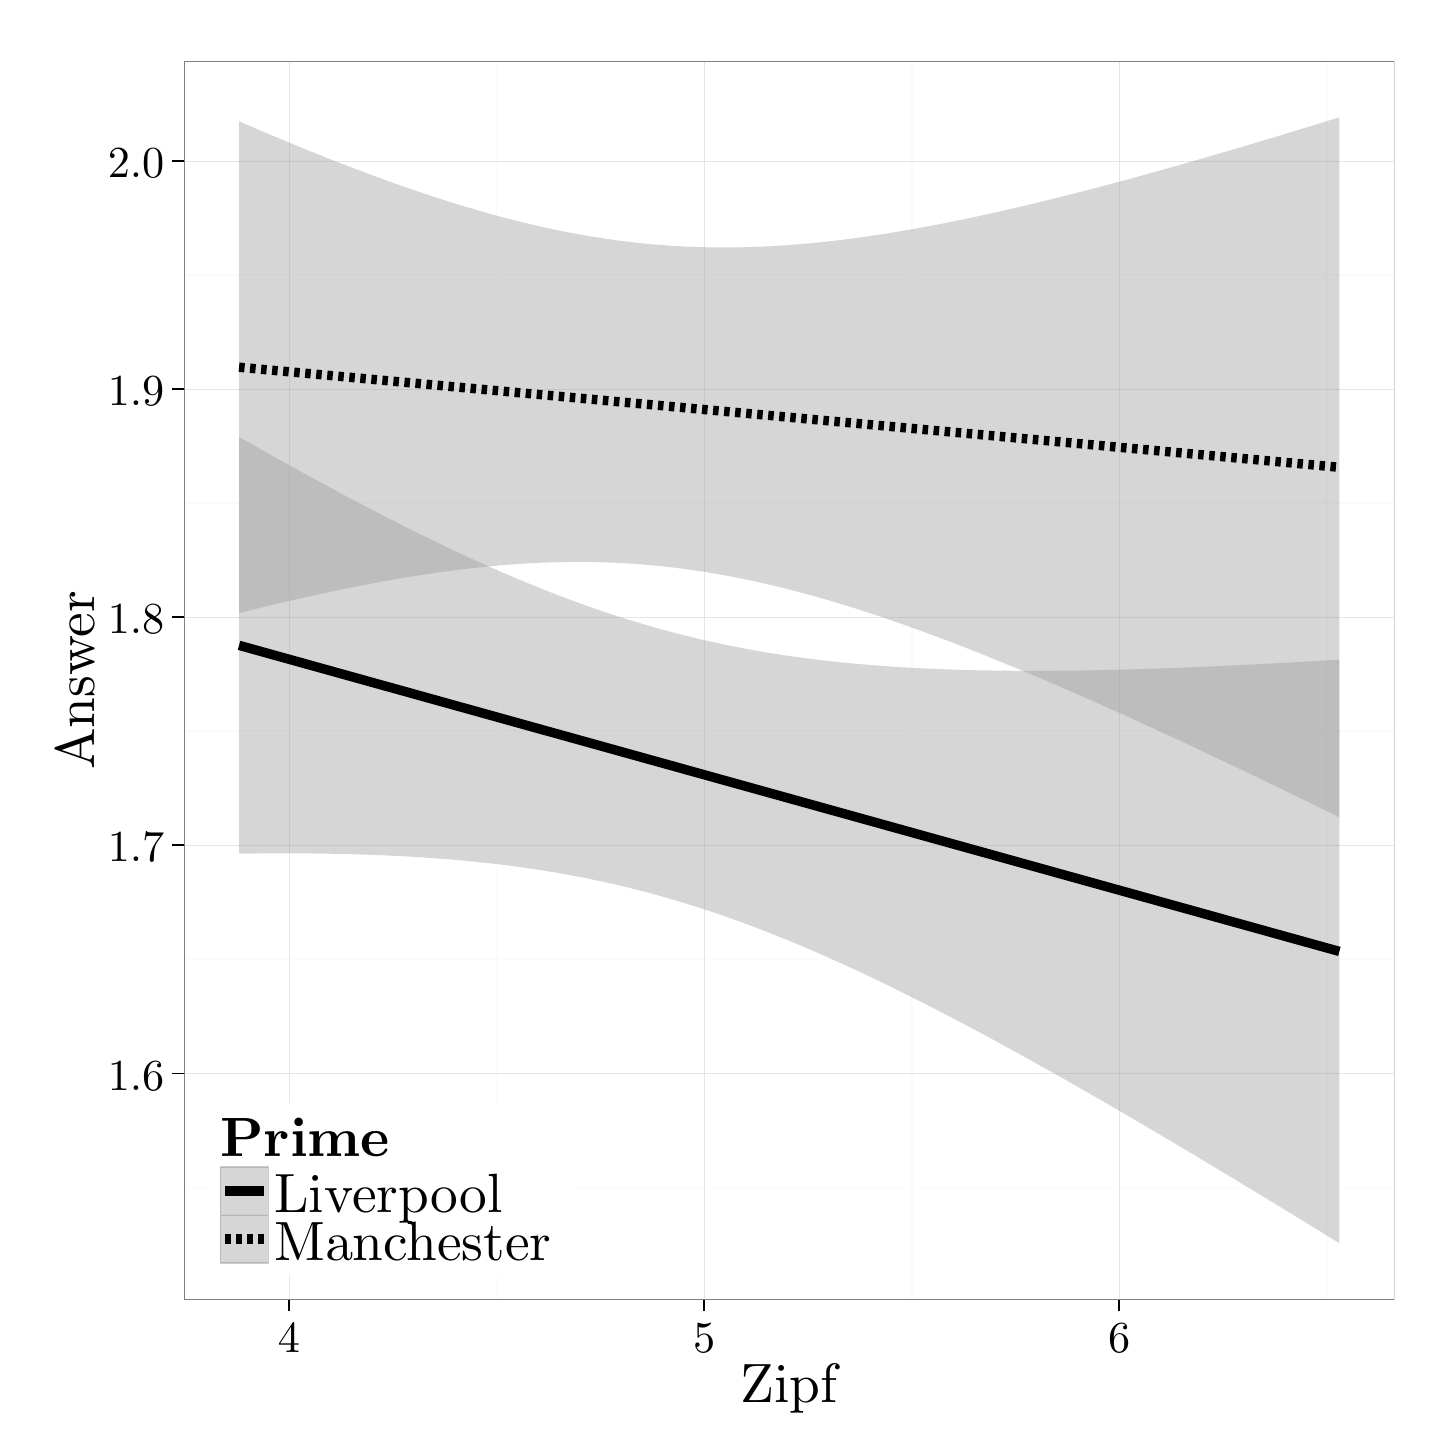
\begin{tikzpicture}[x=1pt,y=1pt]
\definecolor{fillColor}{RGB}{255,255,255}
\path[use as bounding box,fill=fillColor,fill opacity=0.00] (0,0) rectangle (505.89,505.89);
\begin{scope}
\path[clip] (  0.00,  0.00) rectangle (505.89,505.89);
\definecolor{drawColor}{RGB}{255,255,255}
\definecolor{fillColor}{RGB}{255,255,255}

\path[draw=drawColor,line width= 0.6pt,line join=round,line cap=round,fill=fillColor] (  0.00, -0.00) rectangle (505.89,505.89);
\end{scope}
\begin{scope}
\path[clip] ( 56.50, 46.31) rectangle (493.85,493.84);
\definecolor{fillColor}{RGB}{255,255,255}

\path[fill=fillColor] ( 56.50, 46.31) rectangle (493.85,493.84);
\definecolor{drawColor}{gray}{0.98}

\path[draw=drawColor,line width= 0.6pt,line join=round] ( 56.50, 86.79) --
	(493.85, 86.79);

\path[draw=drawColor,line width= 0.6pt,line join=round] ( 56.50,169.23) --
	(493.85,169.23);

\path[draw=drawColor,line width= 0.6pt,line join=round] ( 56.50,251.66) --
	(493.85,251.66);

\path[draw=drawColor,line width= 0.6pt,line join=round] ( 56.50,334.09) --
	(493.85,334.09);

\path[draw=drawColor,line width= 0.6pt,line join=round] ( 56.50,416.53) --
	(493.85,416.53);

\path[draw=drawColor,line width= 0.6pt,line join=round] (169.40, 46.31) --
	(169.40,493.84);

\path[draw=drawColor,line width= 0.6pt,line join=round] (319.43, 46.31) --
	(319.43,493.84);

\path[draw=drawColor,line width= 0.6pt,line join=round] (469.46, 46.31) --
	(469.46,493.84);
\definecolor{drawColor}{gray}{0.90}

\path[draw=drawColor,line width= 0.2pt,line join=round] ( 56.50,128.01) --
	(493.85,128.01);

\path[draw=drawColor,line width= 0.2pt,line join=round] ( 56.50,210.44) --
	(493.85,210.44);

\path[draw=drawColor,line width= 0.2pt,line join=round] ( 56.50,292.88) --
	(493.85,292.88);

\path[draw=drawColor,line width= 0.2pt,line join=round] ( 56.50,375.31) --
	(493.85,375.31);

\path[draw=drawColor,line width= 0.2pt,line join=round] ( 56.50,457.74) --
	(493.85,457.74);

\path[draw=drawColor,line width= 0.2pt,line join=round] ( 94.39, 46.31) --
	( 94.39,493.84);

\path[draw=drawColor,line width= 0.2pt,line join=round] (244.42, 46.31) --
	(244.42,493.84);

\path[draw=drawColor,line width= 0.2pt,line join=round] (394.45, 46.31) --
	(394.45,493.84);
\definecolor{fillColor}{RGB}{153,153,153}

\path[fill=fillColor,fill opacity=0.40] ( 76.38,357.99) --
	( 81.42,355.13) --
	( 86.45,352.28) --
	( 91.48,349.46) --
	( 96.51,346.67) --
	(101.55,343.90) --
	(106.58,341.15) --
	(111.61,338.44) --
	(116.64,335.75) --
	(121.68,333.10) --
	(126.71,330.48) --
	(131.74,327.90) --
	(136.78,325.36) --
	(141.81,322.86) --
	(146.84,320.40) --
	(151.87,317.98) --
	(156.91,315.62) --
	(161.94,313.30) --
	(166.97,311.04) --
	(172.00,308.84) --
	(177.04,306.69) --
	(182.07,304.60) --
	(187.10,302.58) --
	(192.13,300.62) --
	(197.17,298.73) --
	(202.20,296.91) --
	(207.23,295.16) --
	(212.27,293.49) --
	(217.30,291.89) --
	(222.33,290.36) --
	(227.36,288.91) --
	(232.40,287.54) --
	(237.43,286.24) --
	(242.46,285.02) --
	(247.49,283.88) --
	(252.53,282.81) --
	(257.56,281.81) --
	(262.59,280.88) --
	(267.63,280.02) --
	(272.66,279.22) --
	(277.69,278.49) --
	(282.72,277.83) --
	(287.76,277.22) --
	(292.79,276.66) --
	(297.82,276.16) --
	(302.85,275.72) --
	(307.89,275.32) --
	(312.92,274.96) --
	(317.95,274.65) --
	(322.98,274.39) --
	(328.02,274.16) --
	(333.05,273.97) --
	(338.08,273.81) --
	(343.12,273.69) --
	(348.15,273.59) --
	(353.18,273.53) --
	(358.21,273.49) --
	(363.25,273.48) --
	(368.28,273.49) --
	(373.31,273.53) --
	(378.34,273.59) --
	(383.38,273.67) --
	(388.41,273.76) --
	(393.44,273.88) --
	(398.48,274.01) --
	(403.51,274.16) --
	(408.54,274.33) --
	(413.57,274.50) --
	(418.61,274.70) --
	(423.64,274.90) --
	(428.67,275.12) --
	(433.70,275.35) --
	(438.74,275.59) --
	(443.77,275.84) --
	(448.80,276.10) --
	(453.84,276.37) --
	(458.87,276.65) --
	(463.90,276.93) --
	(468.93,277.23) --
	(473.97,277.53) --
	(473.97, 66.65) --
	(468.93, 69.75) --
	(463.90, 72.85) --
	(458.87, 75.94) --
	(453.84, 79.01) --
	(448.80, 82.08) --
	(443.77, 85.14) --
	(438.74, 88.19) --
	(433.70, 91.23) --
	(428.67, 94.26) --
	(423.64, 97.28) --
	(418.61,100.29) --
	(413.57,103.28) --
	(408.54,106.26) --
	(403.51,109.22) --
	(398.48,112.17) --
	(393.44,115.10) --
	(388.41,118.02) --
	(383.38,120.92) --
	(378.34,123.80) --
	(373.31,126.65) --
	(368.28,129.49) --
	(363.25,132.30) --
	(358.21,135.09) --
	(353.18,137.86) --
	(348.15,140.59) --
	(343.12,143.30) --
	(338.08,145.97) --
	(333.05,148.62) --
	(328.02,151.22) --
	(322.98,153.80) --
	(317.95,156.33) --
	(312.92,158.82) --
	(307.89,161.27) --
	(302.85,163.67) --
	(297.82,166.02) --
	(292.79,168.32) --
	(287.76,170.57) --
	(282.72,172.76) --
	(277.69,174.89) --
	(272.66,176.96) --
	(267.63,178.97) --
	(262.59,180.91) --
	(257.56,182.78) --
	(252.53,184.58) --
	(247.49,186.30) --
	(242.46,187.96) --
	(237.43,189.54) --
	(232.40,191.04) --
	(227.36,192.47) --
	(222.33,193.82) --
	(217.30,195.10) --
	(212.27,196.30) --
	(207.23,197.42) --
	(202.20,198.47) --
	(197.17,199.45) --
	(192.13,200.36) --
	(187.10,201.21) --
	(182.07,201.98) --
	(177.04,202.70) --
	(172.00,203.35) --
	(166.97,203.94) --
	(161.94,204.48) --
	(156.91,204.96) --
	(151.87,205.40) --
	(146.84,205.79) --
	(141.81,206.13) --
	(136.78,206.42) --
	(131.74,206.68) --
	(126.71,206.90) --
	(121.68,207.08) --
	(116.64,207.23) --
	(111.61,207.35) --
	(106.58,207.43) --
	(101.55,207.49) --
	( 96.51,207.52) --
	( 91.48,207.52) --
	( 86.45,207.50) --
	( 81.42,207.46) --
	( 76.38,207.39) --
	cycle;
\definecolor{drawColor}{RGB}{0,0,0}

\path[draw=drawColor,line width= 3.4pt,line join=round] ( 76.38,282.69) --
	( 81.42,281.29) --
	( 86.45,279.89) --
	( 91.48,278.49) --
	( 96.51,277.09) --
	(101.55,275.69) --
	(106.58,274.29) --
	(111.61,272.89) --
	(116.64,271.49) --
	(121.68,270.09) --
	(126.71,268.69) --
	(131.74,267.29) --
	(136.78,265.89) --
	(141.81,264.49) --
	(146.84,263.09) --
	(151.87,261.69) --
	(156.91,260.29) --
	(161.94,258.89) --
	(166.97,257.49) --
	(172.00,256.09) --
	(177.04,254.69) --
	(182.07,253.29) --
	(187.10,251.89) --
	(192.13,250.49) --
	(197.17,249.09) --
	(202.20,247.69) --
	(207.23,246.29) --
	(212.27,244.89) --
	(217.30,243.49) --
	(222.33,242.09) --
	(227.36,240.69) --
	(232.40,239.29) --
	(237.43,237.89) --
	(242.46,236.49) --
	(247.49,235.09) --
	(252.53,233.69) --
	(257.56,232.29) --
	(262.59,230.89) --
	(267.63,229.49) --
	(272.66,228.09) --
	(277.69,226.69) --
	(282.72,225.29) --
	(287.76,223.89) --
	(292.79,222.49) --
	(297.82,221.09) --
	(302.85,219.69) --
	(307.89,218.29) --
	(312.92,216.89) --
	(317.95,215.49) --
	(322.98,214.09) --
	(328.02,212.69) --
	(333.05,211.29) --
	(338.08,209.89) --
	(343.12,208.49) --
	(348.15,207.09) --
	(353.18,205.69) --
	(358.21,204.29) --
	(363.25,202.89) --
	(368.28,201.49) --
	(373.31,200.09) --
	(378.34,198.69) --
	(383.38,197.29) --
	(388.41,195.89) --
	(393.44,194.49) --
	(398.48,193.09) --
	(403.51,191.69) --
	(408.54,190.29) --
	(413.57,188.89) --
	(418.61,187.49) --
	(423.64,186.09) --
	(428.67,184.69) --
	(433.70,183.29) --
	(438.74,181.89) --
	(443.77,180.49) --
	(448.80,179.09) --
	(453.84,177.69) --
	(458.87,176.29) --
	(463.90,174.89) --
	(468.93,173.49) --
	(473.97,172.09);

\path[fill=fillColor,fill opacity=0.40] ( 76.38,472.02) --
	( 81.42,469.85) --
	( 86.45,467.71) --
	( 91.48,465.60) --
	( 96.51,463.51) --
	(101.55,461.46) --
	(106.58,459.44) --
	(111.61,457.46) --
	(116.64,455.51) --
	(121.68,453.60) --
	(126.71,451.74) --
	(131.74,449.92) --
	(136.78,448.14) --
	(141.81,446.42) --
	(146.84,444.75) --
	(151.87,443.13) --
	(156.91,441.58) --
	(161.94,440.08) --
	(166.97,438.65) --
	(172.00,437.28) --
	(177.04,435.99) --
	(182.07,434.77) --
	(187.10,433.62) --
	(192.13,432.56) --
	(197.17,431.57) --
	(202.20,430.67) --
	(207.23,429.85) --
	(212.27,429.12) --
	(217.30,428.48) --
	(222.33,427.92) --
	(227.36,427.46) --
	(232.40,427.08) --
	(237.43,426.80) --
	(242.46,426.60) --
	(247.49,426.48) --
	(252.53,426.46) --
	(257.56,426.51) --
	(262.59,426.65) --
	(267.63,426.87) --
	(272.66,427.16) --
	(277.69,427.53) --
	(282.72,427.96) --
	(287.76,428.47) --
	(292.79,429.04) --
	(297.82,429.67) --
	(302.85,430.36) --
	(307.89,431.11) --
	(312.92,431.91) --
	(317.95,432.76) --
	(322.98,433.65) --
	(328.02,434.60) --
	(333.05,435.58) --
	(338.08,436.60) --
	(343.12,437.67) --
	(348.15,438.77) --
	(353.18,439.90) --
	(358.21,441.06) --
	(363.25,442.25) --
	(368.28,443.48) --
	(373.31,444.72) --
	(378.34,446.00) --
	(383.38,447.29) --
	(388.41,448.61) --
	(393.44,449.95) --
	(398.48,451.31) --
	(403.51,452.69) --
	(408.54,454.09) --
	(413.57,455.50) --
	(418.61,456.93) --
	(423.64,458.38) --
	(428.67,459.84) --
	(433.70,461.31) --
	(438.74,462.79) --
	(443.77,464.29) --
	(448.80,465.80) --
	(453.84,467.32) --
	(458.87,468.85) --
	(463.90,470.39) --
	(468.93,471.94) --
	(473.97,473.50) --
	(473.97,220.56) --
	(468.93,223.03) --
	(463.90,225.50) --
	(458.87,227.95) --
	(453.84,230.40) --
	(448.80,232.83) --
	(443.77,235.26) --
	(438.74,237.67) --
	(433.70,240.07) --
	(428.67,242.46) --
	(423.64,244.83) --
	(418.61,247.19) --
	(413.57,249.54) --
	(408.54,251.87) --
	(403.51,254.18) --
	(398.48,256.48) --
	(393.44,258.75) --
	(388.41,261.01) --
	(383.38,263.24) --
	(378.34,265.45) --
	(373.31,267.64) --
	(368.28,269.81) --
	(363.25,271.94) --
	(358.21,274.05) --
	(353.18,276.13) --
	(348.15,278.18) --
	(343.12,280.19) --
	(338.08,282.17) --
	(333.05,284.11) --
	(328.02,286.01) --
	(322.98,287.87) --
	(317.95,289.68) --
	(312.92,291.45) --
	(307.89,293.16) --
	(302.85,294.82) --
	(297.82,296.43) --
	(292.79,297.98) --
	(287.76,299.46) --
	(282.72,300.88) --
	(277.69,302.23) --
	(272.66,303.52) --
	(267.63,304.72) --
	(262.59,305.86) --
	(257.56,306.91) --
	(252.53,307.88) --
	(247.49,308.77) --
	(242.46,309.57) --
	(237.43,310.29) --
	(232.40,310.92) --
	(227.36,311.45) --
	(222.33,311.90) --
	(217.30,312.27) --
	(212.27,312.54) --
	(207.23,312.72) --
	(202.20,312.82) --
	(197.17,312.83) --
	(192.13,312.76) --
	(187.10,312.61) --
	(182.07,312.38) --
	(177.04,312.08) --
	(172.00,311.70) --
	(166.97,311.25) --
	(161.94,310.73) --
	(156.91,310.15) --
	(151.87,309.51) --
	(146.84,308.81) --
	(141.81,308.05) --
	(136.78,307.25) --
	(131.74,306.39) --
	(126.71,305.48) --
	(121.68,304.53) --
	(116.64,303.54) --
	(111.61,302.51) --
	(106.58,301.44) --
	(101.55,300.34) --
	( 96.51,299.20) --
	( 91.48,298.03) --
	( 86.45,296.83) --
	( 81.42,295.61) --
	( 76.38,294.36) --
	cycle;

\path[draw=drawColor,line width= 3.4pt,dash pattern=on 2pt off 2pt ,line join=round] ( 76.38,383.19) --
	( 81.42,382.73) --
	( 86.45,382.27) --
	( 91.48,381.82) --
	( 96.51,381.36) --
	(101.55,380.90) --
	(106.58,380.44) --
	(111.61,379.98) --
	(116.64,379.53) --
	(121.68,379.07) --
	(126.71,378.61) --
	(131.74,378.15) --
	(136.78,377.70) --
	(141.81,377.24) --
	(146.84,376.78) --
	(151.87,376.32) --
	(156.91,375.86) --
	(161.94,375.41) --
	(166.97,374.95) --
	(172.00,374.49) --
	(177.04,374.03) --
	(182.07,373.58) --
	(187.10,373.12) --
	(192.13,372.66) --
	(197.17,372.20) --
	(202.20,371.75) --
	(207.23,371.29) --
	(212.27,370.83) --
	(217.30,370.37) --
	(222.33,369.91) --
	(227.36,369.46) --
	(232.40,369.00) --
	(237.43,368.54) --
	(242.46,368.08) --
	(247.49,367.63) --
	(252.53,367.17) --
	(257.56,366.71) --
	(262.59,366.25) --
	(267.63,365.80) --
	(272.66,365.34) --
	(277.69,364.88) --
	(282.72,364.42) --
	(287.76,363.96) --
	(292.79,363.51) --
	(297.82,363.05) --
	(302.85,362.59) --
	(307.89,362.13) --
	(312.92,361.68) --
	(317.95,361.22) --
	(322.98,360.76) --
	(328.02,360.30) --
	(333.05,359.84) --
	(338.08,359.39) --
	(343.12,358.93) --
	(348.15,358.47) --
	(353.18,358.01) --
	(358.21,357.56) --
	(363.25,357.10) --
	(368.28,356.64) --
	(373.31,356.18) --
	(378.34,355.73) --
	(383.38,355.27) --
	(388.41,354.81) --
	(393.44,354.35) --
	(398.48,353.89) --
	(403.51,353.44) --
	(408.54,352.98) --
	(413.57,352.52) --
	(418.61,352.06) --
	(423.64,351.61) --
	(428.67,351.15) --
	(433.70,350.69) --
	(438.74,350.23) --
	(443.77,349.78) --
	(448.80,349.32) --
	(453.84,348.86) --
	(458.87,348.40) --
	(463.90,347.94) --
	(468.93,347.49) --
	(473.97,347.03);
\definecolor{drawColor}{gray}{0.50}

\path[draw=drawColor,line width= 0.6pt,line join=round,line cap=round] ( 56.50, 46.31) rectangle (493.85,493.84);
\end{scope}
\begin{scope}
\path[clip] (  0.00,  0.00) rectangle (505.89,505.89);
\definecolor{drawColor}{RGB}{0,0,0}

\node[text=drawColor,anchor=base east,inner sep=0pt, outer sep=0pt, scale=  1.60] at ( 49.39,121.98) {1.6};

\node[text=drawColor,anchor=base east,inner sep=0pt, outer sep=0pt, scale=  1.60] at ( 49.39,204.41) {1.7};

\node[text=drawColor,anchor=base east,inner sep=0pt, outer sep=0pt, scale=  1.60] at ( 49.39,286.84) {1.8};

\node[text=drawColor,anchor=base east,inner sep=0pt, outer sep=0pt, scale=  1.60] at ( 49.39,369.28) {1.9};

\node[text=drawColor,anchor=base east,inner sep=0pt, outer sep=0pt, scale=  1.60] at ( 49.39,451.71) {2.0};
\end{scope}
\begin{scope}
\path[clip] (  0.00,  0.00) rectangle (505.89,505.89);
\definecolor{drawColor}{RGB}{0,0,0}

\path[draw=drawColor,line width= 0.6pt,line join=round] ( 52.24,128.01) --
	( 56.50,128.01);

\path[draw=drawColor,line width= 0.6pt,line join=round] ( 52.24,210.44) --
	( 56.50,210.44);

\path[draw=drawColor,line width= 0.6pt,line join=round] ( 52.24,292.88) --
	( 56.50,292.88);

\path[draw=drawColor,line width= 0.6pt,line join=round] ( 52.24,375.31) --
	( 56.50,375.31);

\path[draw=drawColor,line width= 0.6pt,line join=round] ( 52.24,457.74) --
	( 56.50,457.74);
\end{scope}
\begin{scope}
\path[clip] (  0.00,  0.00) rectangle (505.89,505.89);
\definecolor{drawColor}{RGB}{0,0,0}

\path[draw=drawColor,line width= 0.6pt,line join=round] ( 94.39, 42.04) --
	( 94.39, 46.31);

\path[draw=drawColor,line width= 0.6pt,line join=round] (244.42, 42.04) --
	(244.42, 46.31);

\path[draw=drawColor,line width= 0.6pt,line join=round] (394.45, 42.04) --
	(394.45, 46.31);
\end{scope}
\begin{scope}
\path[clip] (  0.00,  0.00) rectangle (505.89,505.89);
\definecolor{drawColor}{RGB}{0,0,0}

\node[text=drawColor,anchor=base,inner sep=0pt, outer sep=0pt, scale=  1.60] at ( 94.39, 27.13) {4};

\node[text=drawColor,anchor=base,inner sep=0pt, outer sep=0pt, scale=  1.60] at (244.42, 27.13) {5};

\node[text=drawColor,anchor=base,inner sep=0pt, outer sep=0pt, scale=  1.60] at (394.45, 27.13) {6};
\end{scope}
\begin{scope}
\path[clip] (  0.00,  0.00) rectangle (505.89,505.89);
\definecolor{drawColor}{RGB}{0,0,0}

\node[text=drawColor,anchor=base,inner sep=0pt, outer sep=0pt, scale=  2.00] at (275.17,  9.03) {Zipf};
\end{scope}
\begin{scope}
\path[clip] (  0.00,  0.00) rectangle (505.89,505.89);
\definecolor{drawColor}{RGB}{0,0,0}

\node[text=drawColor,rotate= 90.00,anchor=base,inner sep=0pt, outer sep=0pt, scale=  2.00] at ( 24.12,270.08) {Answer};
\end{scope}
\begin{scope}
\path[clip] (  0.00,  0.00) rectangle (505.89,505.89);
\definecolor{fillColor}{RGB}{255,255,255}

\path[fill=fillColor] ( 65.37, 55.18) rectangle (198.29,117.15);
\end{scope}
\begin{scope}
\path[clip] (  0.00,  0.00) rectangle (505.89,505.89);
\definecolor{drawColor}{RGB}{0,0,0}

\node[text=drawColor,anchor=base west,inner sep=0pt, outer sep=0pt, scale=  2.00] at ( 69.64, 98.13) {\bfseries Prime};
\end{scope}
\begin{scope}
\path[clip] (  0.00,  0.00) rectangle (505.89,505.89);
\definecolor{drawColor}{gray}{0.80}
\definecolor{fillColor}{RGB}{255,255,255}

\path[draw=drawColor,line width= 0.6pt,line join=round,line cap=round,fill=fillColor] ( 69.64, 76.79) rectangle ( 86.98, 94.13);
\end{scope}
\begin{scope}
\path[clip] (  0.00,  0.00) rectangle (505.89,505.89);
\definecolor{fillColor}{RGB}{153,153,153}

\path[fill=fillColor,fill opacity=0.40] ( 69.64, 76.79) rectangle ( 86.98, 94.13);
\definecolor{drawColor}{RGB}{0,0,0}

\path[draw=drawColor,line width= 3.4pt,line join=round] ( 71.37, 85.46) -- ( 85.25, 85.46);
\end{scope}
\begin{scope}
\path[clip] (  0.00,  0.00) rectangle (505.89,505.89);
\definecolor{drawColor}{gray}{0.80}
\definecolor{fillColor}{RGB}{255,255,255}

\path[draw=drawColor,line width= 0.6pt,line join=round,line cap=round,fill=fillColor] ( 69.64, 59.44) rectangle ( 86.98, 76.79);
\end{scope}
\begin{scope}
\path[clip] (  0.00,  0.00) rectangle (505.89,505.89);
\definecolor{fillColor}{RGB}{153,153,153}

\path[fill=fillColor,fill opacity=0.40] ( 69.64, 59.44) rectangle ( 86.98, 76.79);
\definecolor{drawColor}{RGB}{0,0,0}

\path[draw=drawColor,line width= 3.4pt,dash pattern=on 2pt off 2pt ,line join=round] ( 71.37, 68.12) -- ( 85.25, 68.12);
\end{scope}
\begin{scope}
\path[clip] (  0.00,  0.00) rectangle (505.89,505.89);
\definecolor{drawColor}{RGB}{0,0,0}

\node[text=drawColor,anchor=base west,inner sep=0pt, outer sep=0pt, scale=  2.00] at ( 89.15, 77.92) {Liverpool};
\end{scope}
\begin{scope}
\path[clip] (  0.00,  0.00) rectangle (505.89,505.89);
\definecolor{drawColor}{RGB}{0,0,0}

\node[text=drawColor,anchor=base west,inner sep=0pt, outer sep=0pt, scale=  2.00] at ( 89.15, 60.57) {Manchester};
\end{scope}
\end{tikzpicture}
} 
	\caption{/k/ (perception) by Zipf score}
	\label{fig.scatter.k.ext.zipf}
\end{figure}

For the sake of completeness, we will also have a very brief look at frequency.
Figure \ref{fig.scatter.k.ext.zipf} is another regression plot, this time with frequency measured in \isi{Zipf} scores on the x-axis.
Again, the two lines are not too different in slope, although the decline in the `\isi{Liverpool}' group is somewhat steeper.
In both \isi{priming} conditions, estimated answer token decreases slightly with increasing frequency.
This is the exact opposite of what was found for happ\textsc{y} responses, where there was a positive correlation of estimated answer and frequency (cf. Figure \ref{fig.scatter.happy.ext.zipf}).
For the /k/ responses we \emph{might} argue that higher word frequencies could coincide with higher familiarity (i.e. more (recent) exemplars), which, in turn, may lead to higher accuracy in perception, and translate into lower-numbered answer tokens (see the discussion of the role of distance just above).
With regard to the happ\textsc{y} results, however, this would not work, since the direction of the effect is inverted.
I have no explanation to offer at this point which would cover both results, but two things should be borne in mind:
\begin{inparaenum}[(a)]
	\item The general problems of using frequency as a predictor in this study (cf. Section \ref{sec.perc_method.sentences}), and
	\item the fact that frequency does not end up as a significant fixed effect in the regression model anyway.
\end{inparaenum}
Chances are that what seems to be a (marginally significant) effect of frequency is really due to lexical effects of individual carrier words.